%%%%%%%%%%%%%%%%%%%%%%%%%%%%%%%%%%%%%%%%%
% Oliver Lemon made minor edits (jan 2015)  to : 
% Masters/Doctoral Thesis 
% LaTeX Template
% Version 1.43 (17/5/14)
%
% This template has been downloaded from:
% http://www.LaTeXTemplates.com
%
% Original authors:
% Steven Gunn 
% http://users.ecs.soton.ac.uk/srg/softwaretools/document/templates/
% and
% Sunil Patel
% http://www.sunilpatel.co.uk/thesis-template/
%
% License:
% CC BY-NC-SA 3.0 (http://creativecommons.org/licenses/by-nc-sa/3.0/)
%
% Note:
% Make sure to edit document variables in the Thesis.cls file
%
%%%%%%%%%%%%%%%%%%%%%%%%%%%%%%%%%%%%%%%%%

%----------------------------------------------------------------------------------------
%	PACKAGES AND OTHER DOCUMENT CONFIGURATIONS
%----------------------------------------------------------------------------------------

\documentclass[12pt, oneside]{Thesis} % The default font size and one-sided printing (no margin offsets)

\graphicspath{{Pictures/}} % Specifies the directory where pictures are stored

\usepackage[en-GB]{datetime2}


%paragraph indentation
\setlength{\parindent}{3em} 

\setcounter{tocdepth}{2}

\usepackage[square, sort&compress]{natbib} % Use the natbib reference package - read up on this to edit the reference style; if you want text (e.g. Smith et al., 2012) for the in-text references (instead of numbers), remove 'numbers' 
\hypersetup{urlcolor=blue, colorlinks=true} % Colors hyperlinks in blue - change to black if annoying
\renewcommand\bibname{References}

\expandafter\def\expandafter\UrlBreaks\expandafter{\UrlBreaks%  save the current one
	\do\a\do\b\do\c\do\d\do\e\do\f\do\g\do\h\do\i\do\j%
	\do\k\do\l\do\m\do\n\do\o\do\p\do\q\do\r\do\s\do\t%
	\do\u\do\v\do\w\do\x\do\y\do\z\do\A\do\B\do\C\do\D%
	\do\E\do\F\do\G\do\H\do\I\do\J\do\K\do\L\do\M\do\N%
	\do\O\do\P\do\Q\do\R\do\S\do\T\do\U\do\V\do\W\do\X%
	\do\Y\do\Z}

\usepackage{pdfpages} 
\usepackage{pdflscape}

\usepackage{wrapfig}

%\newcommand{\specialcell}[2][c]{%
%	\begin{tabular}[#1]{@{}c@{}}#2\end{tabular}}

\newcommand{\specialcell}[3][c]{% 		
	\begin{tabular}[#1]{@{}#2@{}}#3\end{tabular}}%

\usepackage{dirtytalk}

\usepackage{verbatim}

\usepackage{float}
%\usepackage[demo]{graphicx}
%\usepackage{caption}
\usepackage{subcaption}

\usepackage{tikz}
\def\checkmark{\tikz\fill[scale=0.4](0,.35) -- (.25,0) -- (1,.7) -- (.25,.15) -- cycle;} 

\usepackage{soul}
\newcommand{\hlc}[2][pink]{ {\sethlcolor{#1} \hl{#2}}}

\title{HWU CS Masters thesis template} % BUT you should use use " \title{\ttitle} " here instead to define the thesis title ! 
% \ttitle is defined in the file Thesis.cls 

\begin{document}

\frontmatter % Use roman page numbering style (i, ii, iii, iv...) for the pre-content pages

\setstretch{1.3} % Line spacing of 1.3

% Define the page headers using the FancyHdr package and set up for one-sided printing
\fancyhead{} % Clears all page headers and footers
\rhead{\thepage} % Sets the right side header to show the page number
\lhead{} % Clears the left side page header

\pagestyle{fancy} % Finally, use the "fancy" page style to implement the FancyHdr headers

\newcommand{\HRule}{\rule{\linewidth}{0.5mm}} % New command to make the lines in the title page

% PDF meta-data
\hypersetup{pdftitle={\ttitle}}
\hypersetup{pdfsubject=\subjectname}
\hypersetup{pdfauthor=\authornames}
\hypersetup{pdfkeywords=\keywordnames}

%----------------------------------------------------------------------------------------
%	TITLE PAGE
%----------------------------------------------------------------------------------------

\begin{titlepage}
\begin{center}

\textsc{\LARGE \univname}\\[1.5cm] % University name
%\textsc{\Large Masters Thesis}\\[0.5cm] % Thesis type

\HRule \\[0.4cm] % Horizontal line
{\LARGE \bfseries {It's More Complicated Than That: \\ \vspace{0.1cm} A Study of Discrepancies Between Industry Guidance and Practice in Building Services Engineers' Processes for Collaboration in the UK}}\\[0.4cm] % Thesis title
\HRule \\[1.5cm] % Horizontal line
 
\begin{minipage}{0.4\textwidth}
\begin{flushleft} \large
\emph{Author:}\\
\authornames % Author name - remove the \href bracket to remove the link
\\ H00165151
\end{flushleft}
\end{minipage}
\begin{minipage}{0.5\textwidth}
\begin{flushright} \large
\emph{Supervisor:} \\
\supname % Supervisor name - remove the \href bracket to remove the link  
\\ BA(Hons) DipArch RIBA FRSA
\end{flushright}
\end{minipage}\\[3cm]
 
\large \textit{A thesis submitted for the degree of \\ \degreename}\\[0.3cm] % University requirement text
\textit{in the}\\[0.4cm]
%\groupname\\

\deptname\\[1cm] % Research group name and department name
 
{\large \DTMlangsetup{showdayofmonth=false} \today}\\[1cm] % Date

\includegraphics[width=4.5cm]{./figures/HWlogo2016.jpg} % University/department logo - uncomment to place it
 
\vfill
\end{center}

\end{titlepage}

%----------------------------------------------------------------------------------------
%	DECLARATION PAGE
%	Your institution may give you a different text to place here
%----------------------------------------------------------------------------------------

\Declaration{

\addtocontents{toc}{\vspace{1em}} % Add a gap in the Contents, for aesthetics

I, \authornames, declare that this thesis titled, `\ttitle' and the work presented in it is my own. I confirm that this work submitted for assessment is my own and is
  expressed in my own words. Any uses made within it of the works of
  other authors in any form (e.g. ideas, equations, figures, text,
  tables, programs) are properly acknowledged at any point of their
  use. A list of the references employed is included.

%\begin{itemize} 
%\item[\tiny{$\blacksquare$}] This work was done wholly or mainly while in candidature for a research degree at this University.
%\item[\tiny{$\blacksquare$}] Where any part of this thesis has previously been submitted for a degree or any other qualification at %this University or any other institution, this has been clearly stated.
%\item[\tiny{$\blacksquare$}] Where I have consulted the published work of others, this is always clearly attributed.
%\item[\tiny{$\blacksquare$}] Where I have quoted from the work of others, the source is always given. With the exception of such %quotations, this thesis is entirely my own work.
%\item[\tiny{$\blacksquare$}] I have acknowledged all main sources of help.
%\item[\tiny{$\blacksquare$}] Where the thesis is based on work done by myself jointly with others, I have made clear exactly what %was done by others and what I have contributed myself.\\
%\end{itemize}
 \vspace{2cm} 
Signed: 
\includegraphics[width=3cm]{./figures/Signature.png}\\
\rule[1em]{25em}{0.5pt} % This prints a line for the signature
 
Date: \today\\
\rule[1em]{25em}{0.5pt} % This prints a line to write the date
}

\clearpage % Start a new page

%----------------------------------------------------------------------------------------
%	QUOTATION PAGE
%----------------------------------------------------------------------------------------

\pagestyle{empty} % No headers or footers for the following pages

\null\vfill % Add some space to move the quote down the page a bit

\textit{``Teamwork is the ability to work together toward a common vision. The ability to direct individual accomplishments toward organizational objectives. It is the fuel that allows common people to attain uncommon results."}

\begin{flushright}
Andrew Carnegie
\end{flushright}

\vfill\vfill\vfill\vfill\vfill\vfill\null % Add some space at the bottom to position the quote just right

\clearpage % Start a new page

%----------------------------------------------------------------------------------------
%	ABSTRACT PAGE
%----------------------------------------------------------------------------------------

\addtotoc{Abstract} % Add the "Abstract" page entry to the Contents

%\abstract{\addtocontents{toc}{\vspace{1em}} % Add a gap in the Contents, for aesthetics

 {\huge{\textit{Abstract}} \par}{\addtocontents{toc}{\vspace{1em}} 

Building Information Modelling (BIM) is a recent innovation in technology and process that has been introduced to the UK's architecture, engineering and construction (AEC) industry as a means to increase collaboration and productivity.
This dissertation assesses the effectiveness and implications of the industry's guidance for the adoption of BIM in the context of building services engineering by identifying discrepancies with practising engineers' collaborative experiences with BIM.
Collaboration-related issues that have been experienced by building services engineers were firstly scoped out through conversations with two AEC professionals in building services.
Thereafter, the industry's authoritative BIM guidance documents were examined and a questionnaire designed to assess the extent of practising building services engineers' compliance and issues with the guidance.
%  and identify the collaboration-related issues in their BIM adoption.
% The survey consisted  of 40 AEC professionals who are or have interacted with building services engineers
Follow-up interviews were conducted with two of the survey respondents to gain deeper insights and a more complete picture of practising engineers' collaborative experiences with BIM.
% Data about collaborative experiences with practising building services engineers was then collected through a survey that was predicated on a review of the 
% The author then designed a questionnaire for practising AEC professionals who are or have interacted with building services engineers that was predicated on the 
The study revealed five discrepancies between industry guidance and practice regarding
% These discrepancies 
% highlighted issues in 
the awareness and knowledge of BIM,
software interoperability, 
the differing skill sets of consultants and contractors,
the persistent use of proprietary file formats,
and the ambiguity of levels of definition (LODs).
The discrepancies raised questions regarding the value in streamlining the building services consultant-to-contractor handover, as is recommended by the industry.
They also suggested potentially necessary reformations of consultants' and contractors' roles in the building services industry, and of LODs for more effective communication in BIM.

%The page is kept centered vertically so can expand into the blank space above the title too\ldots
%

{\vspace{2em}
\noindent
\textit{Keywords:}
BG 6;
BIM;
building information modelling;
communication;
consultant-to-contractor handover;
information flow patterns;
interoperability;
levels of definition;
LOD;
mechanical, electrical and public health engineering;
MEP;
PAS 1192-2.
}


\clearpage % Start a new page

%----------------------------------------------------------------------------------------
%	ACKNOWLEDGEMENTS
%----------------------------------------------------------------------------------------

\setstretch{1.3} % Reset the line-spacing to 1.3 for body text (if it has changed)

\acknowledgements{\addtocontents{toc}{\vspace{1em}} % Add a gap in the Contents, for aesthetics

I would like to thank my supervisor, Alex MacLaren, for her friendly guidance, useful insights, and enthusiasm throughout this endeavour.
I am also exceptionally grateful to Darren Quigley, Paddy Conaghan, Britta Kalkreuter, Martin Howe and Mark Wallace for the time they gave up to speak with me and share their insights into my research study.
Thank you to David Kelly and Amna Malik for testing my questionnaire, and to the forty AEC professionals who took time out of their busy schedules to complete my survey.
I am also much obliged to Les Copeland, who provided me with copies of the latest ACE Schedule of Services MEP editions through Paddy Conaghan.
And lastly, I would like to thank Max Baird for his unfaltering support.
}

\clearpage % Start a new page

%----------------------------------------------------------------------------------------
%	LIST OF CONTENTS/FIGURES/TABLES PAGES
%----------------------------------------------------------------------------------------

\pagestyle{fancy} % The page style headers have been "empty" all this time, now use the "fancy" headers as defined before to bring them back

\lhead{\emph{Contents}} % Set the left side page header to "Contents"
\tableofcontents % Write out the Table of Contents

\lhead{\emph{List of Figures}} % Set the left side page header to "List of Figures"
\listoffigures % Write out the List of Figures

\lhead{\emph{List of Tables}} % Set the left side page header to "List of Tables"
\listoftables % Write out the List of Tables

%----------------------------------------------------------------------------------------
%	ABBREVIATIONS
%----------------------------------------------------------------------------------------

\clearpage % Start a new page

\setstretch{1.5} % Set the line spacing to 1.5, this makes the following tables easier to read

\lhead{\emph{Abbreviations}} % Set the left side page header to "Abbreviations"
\listofsymbols{ll} % Include a list of Abbreviations (a table of two columns)
{
\textbf{AE} & \textbf{A}rchitectural \textbf{E}ngineering \\
%
\textbf{CAD} & \textbf{C}omputer-\textbf{A}ided \textbf{D}esign \\
}

%----------------------------------------------------------------------------------------
%	PHYSICAL CONSTANTS/OTHER DEFINITIONS
%----------------------------------------------------------------------------------------

%\clearpage % Start a new page

%\lhead{\emph{Physical Constants}} % Set the left side page header to "Physical Constants"

%\listofconstants{lrcl} % Include a list of Physical Constants (a four column table)
%{
%Speed of Light & $c$ & $=$ & $2.997\ 924\ 58\times10^{8}\ \mbox{ms}^{-\mbox{s}}$ (exact)\\

%% Constant Name & Symbol & = & Constant Value (with units) \\
%}

%----------------------------------------------------------------------------------------
%	SYMBOLS
%----------------------------------------------------------------------------------------

\clearpage % Start a new page

%\lhead{\emph{Symbols}} % Set the left side page header to "Symbols"

\listofnomenclature{lll} % Include a list of Symbols (a three column table)
{
$a$ & distance & m \\
$P$ & power & W (Js$^{-1}$) \\
% Symbol & Name & Unit \\

& & \\ % Gap to separate the Roman symbols from the Greek

$\omega$ & angular frequency & rads$^{-1}$ \\
% Symbol & Name & Unit \\
}

%----------------------------------------------------------------------------------------
%	DEDICATION
%----------------------------------------------------------------------------------------

\setstretch{1.3} % Return the line spacing back to 1.3

\pagestyle{empty} % Page style needs to be empty for this page

\dedicatory{For Max\ldots} % Dedication text

\addtocontents{toc}{\vspace{2em}} % Add a gap in the Contents, for aesthetics

%----------------------------------------------------------------------------------------
%	THESIS CONTENT - CHAPTERS
%----------------------------------------------------------------------------------------

\mainmatter % Begin numeric (1,2,3...) page numbering

\pagestyle{fancy} % Return the page headers back to the "fancy" style

% Include the chapters of the thesis as separate files from the Chapters folder
% Uncomment the lines as you write the chapters

\chapter{Introduction} % Main chapter title

\label{Chapter1} % Change X to a consecutive number; for referencing this chapter elsewhere, use \ref{ChapterX}

\lhead{Chapter 1. \emph{Introduction}} % Change X to a consecutive number; this is for the header on each page - perhaps a shortened title

Test
\chapter{Literature Review} % Main chapter title

\label{Chapter2} % Change X to a consecutive number; for referencing this chapter elsewhere, use \ref{ChapterX}

\lhead{Chapter 2. \emph{Literature Review}} % Change X to a consecutive number; this is for the header on each page - perhaps a shortened title

The government seems convinced that BIM will solve the problems in the AEC industry through the standardisation of processes and by creating a collaborative culture.
Thus, BIM literature has been reviewed to gain a deeper understanding of BIM, its collaboration-enabling abilities and its adoption in the industry.
%----------------------------------------------------------------------------------------
%	SECTION 1
%----------------------------------------------------------------------------------------

\section{Issues in the Industry}

The AEC industry has recently had a poor reputation due to its poor performance.
An adversarial claims culture emerged within the industry, which often delivered projects that were late, over budget, and of poor quality.
Also, due to a lack of focus on the client, project results tended to drift from the client's original goal.
Hence, this caused an overall dissatisfaction of clients with the AEC industry \citep{lecnotes, Egan1998}.
The poor performance of the industry can largely be attributed to its paradoxical nature; despite the essence of the industry being intense collaborations on bespoke projects in temporary groupings \citep{Laakso2012}, the industry is fragmented, with individual disciplines tending to work in isolation from others \citep{GCS16-20,Miettinen2014}.


%----------------------------------------------------------------------------------------
%	SECTION 2
%----------------------------------------------------------------------------------------

\section{A Call for Collaboration}

In the 1990s, the industry addressed these issues to the UK Government in two key reports: \say{Constructing the Team} by \cite{Latham1994} and \say{Rethinking Construction} by \cite{Egan1998}.
The reports called for a reinvention of the AEC industry to improve its performance and put the client back in the centre.
In order to achieve this, a need for collaboration and standardisation was highlighted.
\cite{Latham1994} and \cite{Egan1998} asked the government to implement their propositions for improvement and to commit itself to becoming a best practice client, thus setting an example for the rest of the industry's clients.


Since then, the government has agreed to become an exemplary client and to implement the reports' propositions.
This is evidenced by a series of documents, including the Government Construction Strategies (GCSs) of 2011-15 by the \cite{GCS11-15} and of 2016-20 by the Infrastructure and Projects Authority \citep{GCS16-20}.
The government's motivations for doing this have been to reduce the cost of its construction projects by up to 20\% and improve the value offered by public sector construction \citep{GCS11-15}.
Amongst the government's strategies for achieving this goal were enabling early contractor and supply chain involvement, standardising products and processes, and replacing adversarial cultures with collaborative ones.
As part of the mobilisation towards collaboration, GCS 2011-15 required Building Information Modelling (BIM) Level 2 as a minimum on all public sector projects by 2016 \citep{GCS11-15}.
Likewise, one of the principal objectives of GCS 2016-20 is to further embed and increase the use of digital technology such as BIM \citep{GCS16-20}.

%----------------------------------------------------------------------------------------
%	SECTION 3
%----------------------------------------------------------------------------------------

\section{BIM} \label{bim}
% Then I'll go on to talk about the facilitators of communication and collaboration. 
% Tools: BIM (Lvl 2 required by 2016 by GCS)
According to the British National Building Specification \citep{NBS2016} and the American National Institute of Building Sciences \citep{NIBSnd}, BIM is the process for creating, managing, and communicating information and knowledge about a built asset throughout its lifecycle, from inception to demolition.
A key output of the process is the building information model (a.k.a. BIM model), a digital file describing every aspect of the built asset.
Overall, literature agrees that the collaborative environment is one of the best aspects of BIM \citep{Santos2017}.
This would explain why the GCSs pushed for the adoption of BIM, believing that it could assist in the reduction of \say{abortive work, discrepancies and mistakes, and inefficiencies in the information supply chain [which] are major contributors to [the industry's] waste} \citep{NBS2014}.

However, the government has recognised that the process of moving the construction industry to `full' collaborative working will be progressive.
Hence, it has defined distinct and recognisable milestones within that process in the form of `levels', as illustrated in Figure \ref{levels}.
Of these levels, the government mandated BIM Level 2 as a minimum on all public sector projects by 2016 \citep{GCS11-15}.
\cite{NBS2014} defines BIM Level 2 as \say{distinguished by collaborative working – all parties use their own 3D CAD models, but not necessarily working on a single, shared model. The collaboration comes in the form of how the information is exchanged between different parties – and is the crucial aspect of this level. Design information is shared through a common file format, which enables any organisation to be able to combine that data with their own in order to make a federated BIM model, and to carry out interrogative checks on it.}

\begin{figure}[htbp]
	\centering
	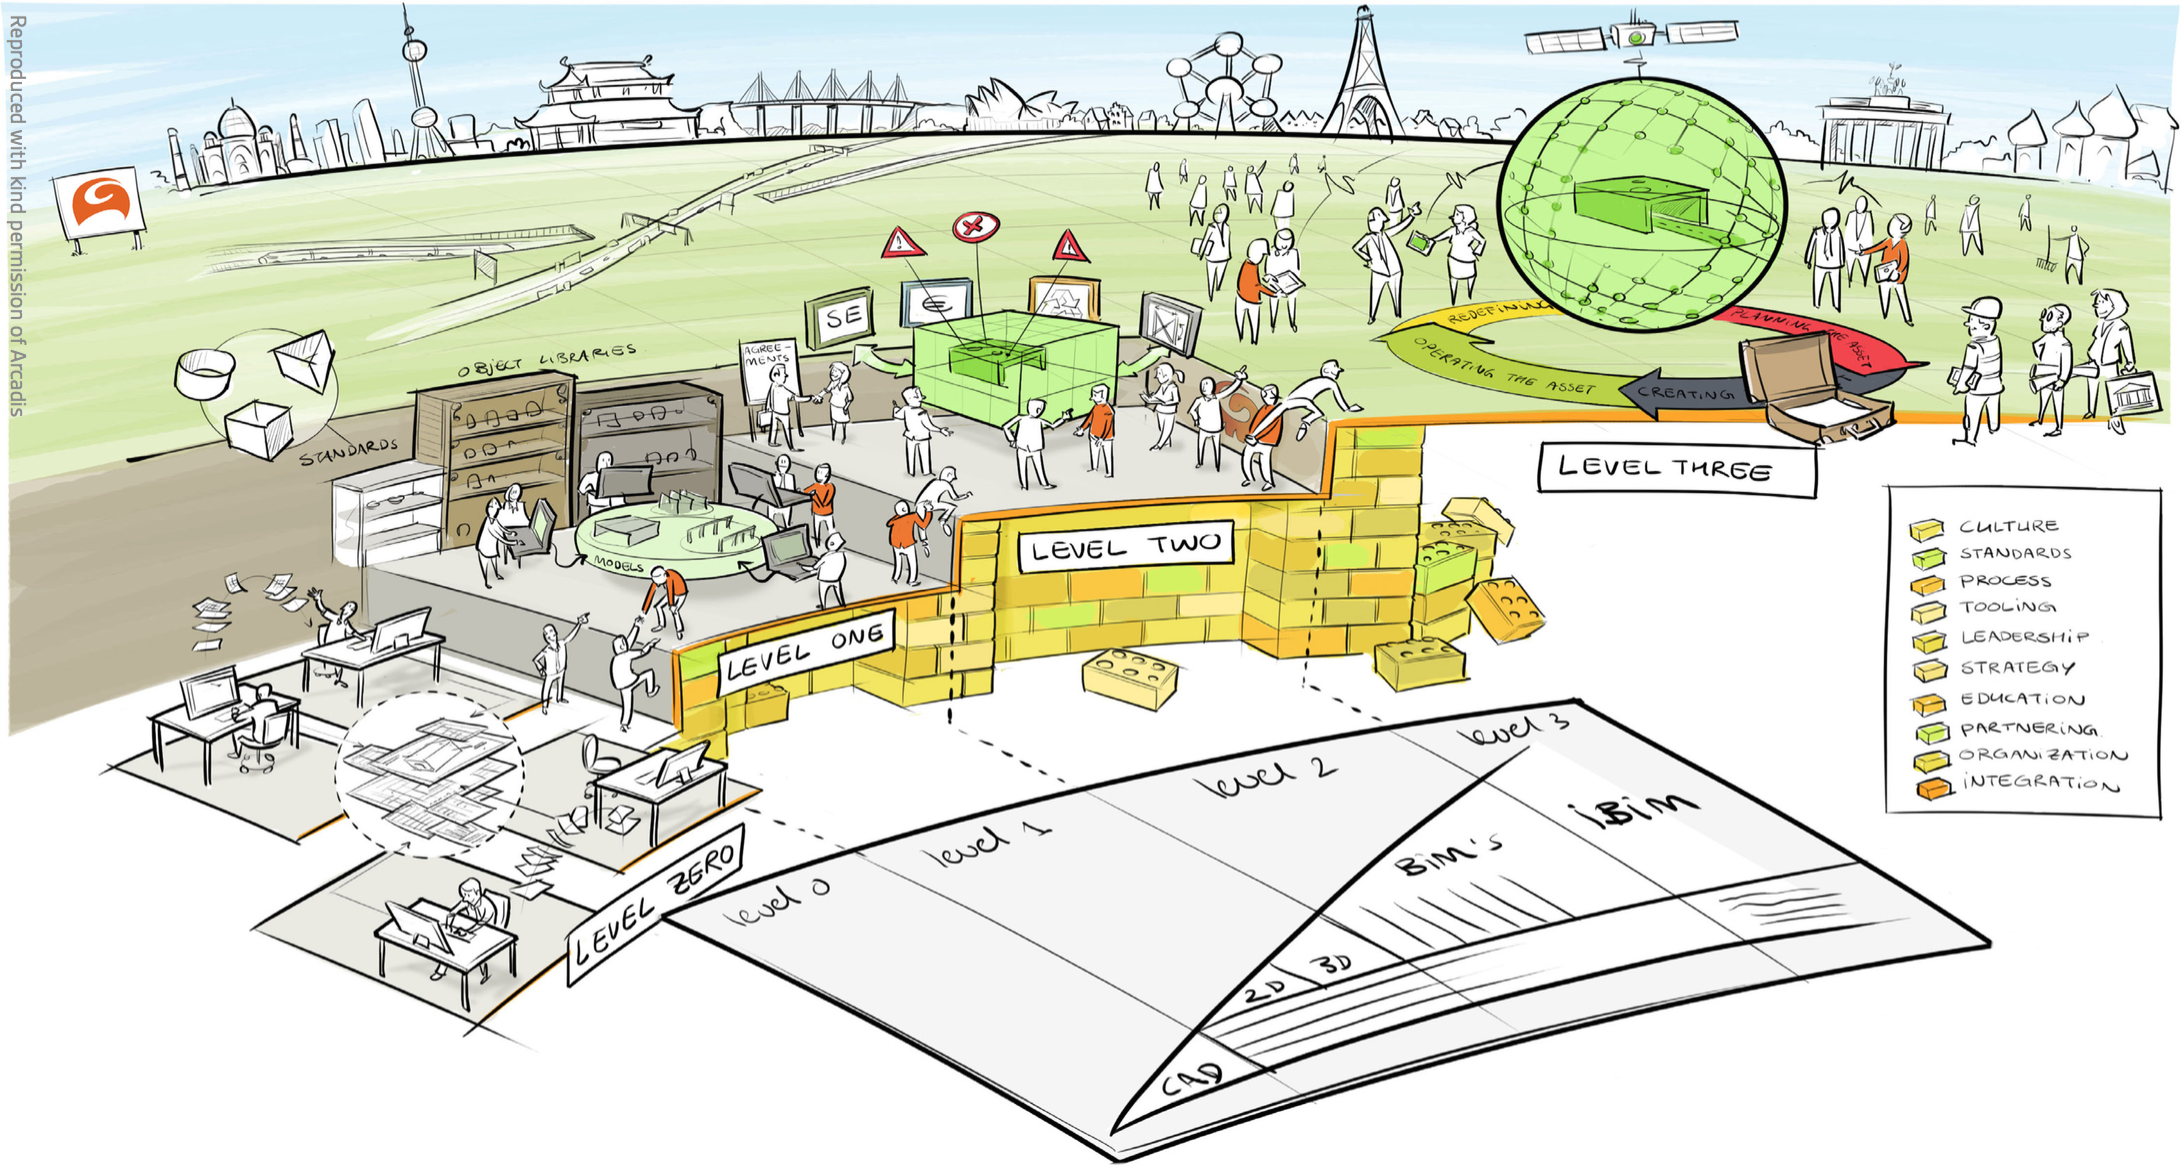
\includegraphics[width=\textwidth]{figures/BIMlevels.png}
	\rule{\textwidth}{0.5pt} % use line???
	\caption[BIM levels]{BIM levels \citep{BSI}.}
	\label{levels}
\end{figure}


As per the government's wish for the standardisation of products and processes, standards have been published and processes established that support the industry's mobilisation towards collaboration.
Processes include the RIBA Plan of Work (PoW) 2013 which \say{provides a framework for the project team to approach design, construction and operational processes} and the BIM Task Group's Digital PoW which \say{aims to provide clarity on how built asset data is defined, tested and successfully used by the supply chain and the public client to achieve BIM Level 2} \citep{Fairhead2015:online}.
Standards have been rapidly developed to meet the immediate market need for BIM Level 2 guidance \citep{NBS2017}.
These rapidly developed standards, a.k.a. Publicly Available Specifications (PAS), and other British Standards (BS) are listed in Figure \ref{stds}.


\begin{figure}[htbp]
	\centering
	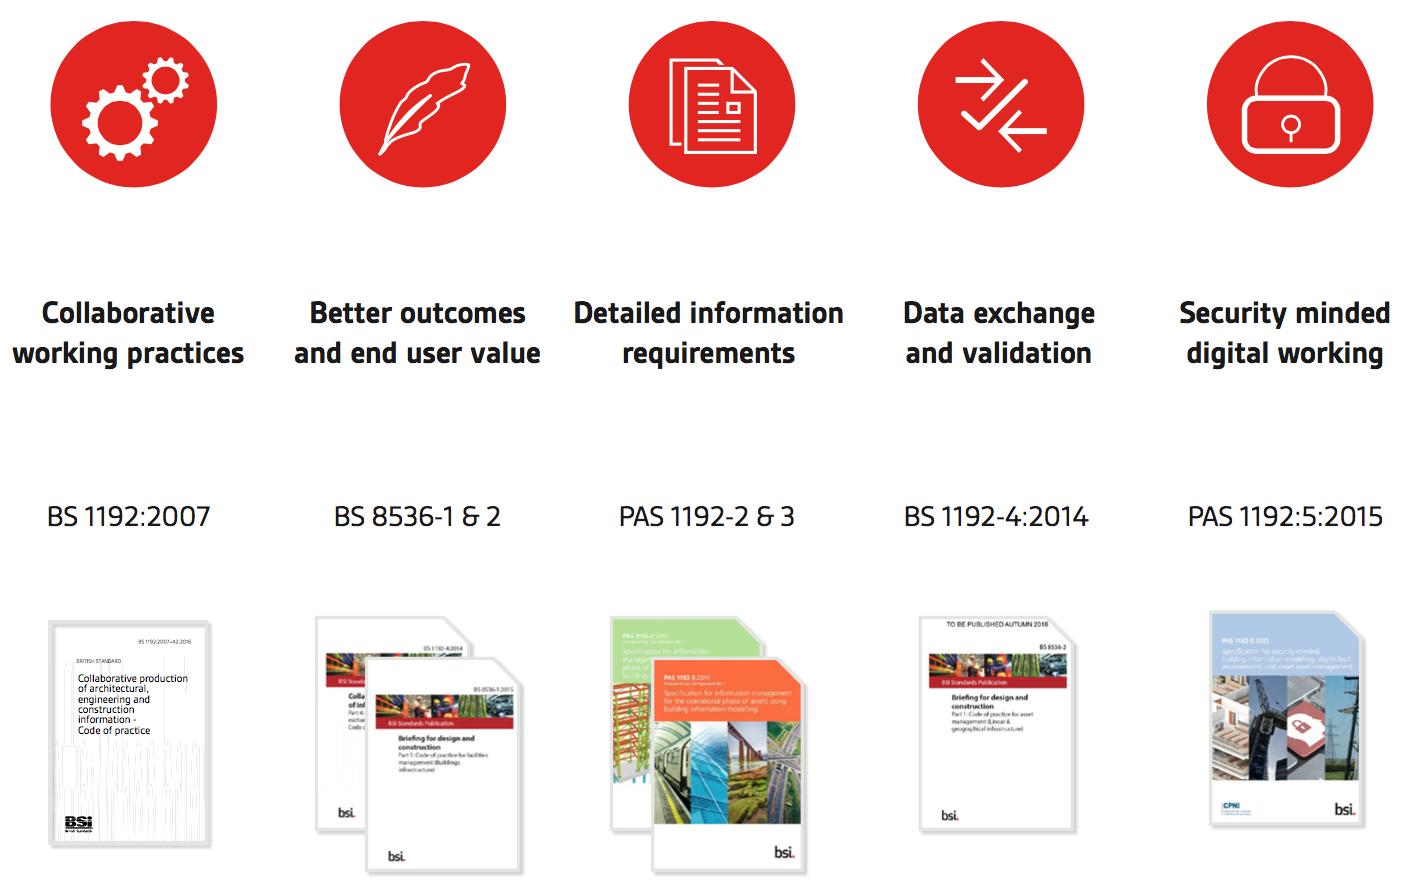
\includegraphics[width=\textwidth]{figures/BIMstandards.png}
	\rule{\textwidth}{0.5pt} % use line???
	\caption[BIM Level 2 British Standards and Publicly Available Specifications]{British Standards (BS) and Publicly Available Specifications (PAS) supporting BIM Level 2 adoption \citep{BSI}.}
	\label{stds}
\end{figure}



%----------------------------------------------------------------------------------------
%	SECTION 4
%----------------------------------------------------------------------------------------

\section{Problems Encountered in the Adoption of BIM}
% After that, the problems faced in the adoption of BIM will be described.
In spite of all the support and protocols, the adoption of BIM has been uneven across the industry.
\cite{DesigningBuildingsLtd2017} suggests that the industry is only helping those at the forefront of BIM adoption get better at it while leaving the rest behind, thus making BIM a specialist subject.

Moving to BIM from pen and paper or computer-aided design (CAD) requires a shift in existing work practices \citep{Singh2011}.
A case study by \cite{Neff2010} gives a couple examples of this shift from the experiences of people in the industry.
Firstly, whereas architects may have appreciated the interpretative flexibility that came with drawings, especially during the conceptual design stages, there is no longer any room for interpretation in BIM models because all the data needs to be inputted exactly.
Secondly, BIM software packages require designers to, for instance, select the colour of a door in the model when it may not yet have been actually decided. 
If the designer were to show that model to the client, the client may get distracted, confused or misled by this `pre-decision'.
Therefore, this over-determination of information that BIM software packages sometimes require can alter or even degrade communication between stakeholders.

Literature shows that there is a reluctance, and sometimes inability, to change existing work practices in order to make the BIM shift.
On the one hand, \cite{Laakso2012} suggest that small companies may not have the resources to adopt BIM.
On the other hand, \cite{Singh2011} suggest that the industry can often find itself stuck in a status quo loop, as illustrated in Figure \ref{loop}.
\say{The lack of knowledge and awareness about BIM can result in a lack of confidence and motivation to adopt BIM-based collaboration. Conversely, as a result of the inhibition to adopt and use BIM, the level of knowledge about BIM remains} \citep[p.~136]{Singh2011}.

\begin{figure}[htbp]
	\centering
	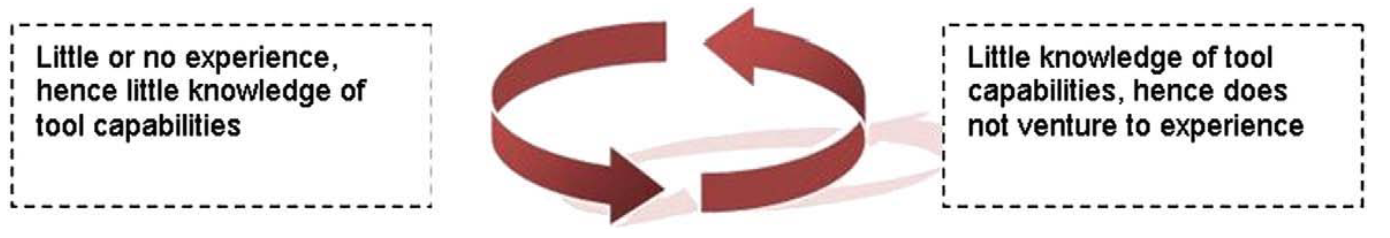
\includegraphics[width=\textwidth]{figures/Loop.png}
	\rule{\textwidth}{0.5pt} % use line???
	\caption[Status quo loop inhibiting BIM adoption]{Status quo loop inhibiting BIM adoption \citep[p.~136]{Singh2011}.}
	\label{loop}
\end{figure}

\noindent
Some other factors that are impeding the adoption of BIM are:
\begin{itemize}
	\item The fragmented nature of the industry \citep{Singh2011,Neff2010} 
	\item A lack of initiative, training and available skilled personnel in BIM \citep{Singh2011,Ghaffarianhoseini2017}
	\item A lack of clarity on roles, responsibilities, and distribution of benefits in adopting the BIM approach \citep{Singh2011,Ghaffarianhoseini2017}
	\item Intellectual property and security-related concerns \citep{Ghaffarianhoseini2017,Laakso2012} 
	\item A lack of interoperability between different pieces of software \citep{GCS11-15,Laakso2012}. 
	(Interoperability is the ability of different software applications to exchange and make use of data \citep{Gallaher2004}.)
\end{itemize}


%------------------------------
%	SUBSECTION 1
%------------------------------

\subsection{A More Realistic View on the Adoption of BIM}
% More sober view of BIM adoption
\cite{Miettinen2014} argue that the industry's expectations of BIM are too high and that the encountered problems are normal in the adoption of a new technology that fundamentally changes how the industry works.
In literature, \cite{Miettinen2014} found a couple reasons for these high expectations.
The first reason is that the promises of the benefits of BIM were initially set high in order to attract financial sponsors and stimulate political agendas.
The second is that there has been a tendency to equate the technological potential of BIM to future reality while ignoring the actual circumstances that are likely to complicate and delay the realisation of that vision.
In fact, \cite{Miettinen2014} claim that it normally takes a company two decades for it to embed a new technology into its work practice from the time the technology is introduced to the company.
% So maybe…


%----------------------------------------------------------------------------------------
%	SECTION 5
%----------------------------------------------------------------------------------------


















\begin{comment}

% CONSTRUCTION INDUSTRY PROBLEMS
The construction industry is highly fragmented \citep{GCS16-20}. 
The construction industry has long been infamous for delivering projects late, over budget or of poor quality. This led to an increase of dissatisfied clients and created an adversarial "claims" culture in the industry. Project outcomes drifted from the original goals due to a lack of focus on the client, poorly defined procurement routes, and contract forms that did not encourage or accommodate colaboration.  (P\&C lec notes)
there is deep concern that the industry as a whole is under-achieving.It has low profitability and invests too little in capital, research and development and training. Too many of the industry's clients are dissatisfied with its overall performance \citep{Egan1998}.


% INDUSTRY TO GOVT: NEED FOR COLLABORATION
Two key joint industry (?) and government reports were published in response to these issues: \say{Constructing the Team} by \cite{Latham1994} and \say{Rethinking Construction} by \cite{Egan1998}. As the reports' titles suggest, these reports called for collaboration and innovation in the construction industry.
\cite{Egan1998} identified five key drivers for change for the industry, one of which was \say{integrated process and teams}. Moreover, \cite{Egan1998} called for standardisation of components and processes in order to \say{design projects for ease of construction}.
Similarly, \cite{Latham1994} called for standardisation by urging clients to start using the New Engineering Contract (NEC) and \say{phase out \say{bespoke} documents}.
Furthermore, both reports asked the government to commit itself to becoming a best practice client and to lead public sector bodies to becoming best practice clients by implementing the reports' propositions and thus setting an example for the rest of the construction industry clients.

% GOVT TO INDUSTRY: OK --> CONDENSE TO 1 PARAGRAPH
The government has since taken action/ responded to the Latham and Egan reports.
The government has published a series of documents with a plan of action of how it and public sector bodies plan to implement Latham's and Egan's propositions, including the Government Construction Strategies (GCS) of 2011-15 \citep{GCS11-15} and 2016-20 \citep{GCS16-20}.
In both of the documents mentioned, the government agrees to become an exemplary client across the industry.

With the ultimate aim of reducing the cost of government construction projects by 15-20\%, GCS 2011-15 identified the need to improve the value offered by public sector construction.
Amongst the strategies of achieving this goal was the promotion of product standardisation and collaborative cultures to replace adversarial ones.
As part of the boration, the report introduced Building Information Modelling (BIM) as offering a \say{a fully collaborative 3D environment, [where] all of those involved in a project are working on a shared platform with reduced transaction costs and less opportunity for error} \citep[p.~13]{GCS11-15}.
Literature supports this, saying that the collaborative environment is one of the best aspects of BIM \citep{Santos2017}.
The report then goes on to say that the \say{Cabinet Office will co-ordinate Government's drive to the development of standards enabling all members of the supply chain to work collaboratively through Building Information Modelling (BIM)}, and that \say{Government will require fully collaborative 3D BIM (with all project and asset information, documentation and data being electronic) as a minimum by 2016} \citep[pp.~13-14]{GCS11-15}.

According to GCS 2016-20, £3 million of efficiency savings were delivered over 2011-15, which was partially enabled by \say{developing new models and approaches to procurement, which focus on collaboration and early contractor involvement} and \say{developing digital capability in design and construction, with all departments on target to procure assets using Building Information Modelling (BIM) Level 2 by 2016} \citep[p.~3]{GCS16-20}.
Following that, two of the four principal objectives of GCS 2016-20 are to (1) embed and increase the use of digital technology, including BIM Level 2, and (2) deploy collaborative procurement techniques that, amongst other objectives, enable early contractor and supply chain involvement \citep[p.~2]{GCS16-20}.

% STDISATION
Compatible tools are vital in an industry such as the construction industry, where several organisations collaborate intensively on bespoke projects in temporary groupings \citep{Laakso2012}.
The best solution would be to have widely accepted and mature technical platforms based on open standards to enable communication and collaboration among project participants without requiring them to have specific proprietary applications.
\say{IFC (Industry Foundation Classes) is an open and standardized data model intended to enable interoperability between building information modeling software applications in the AEC/FM industry} \citep{Laakso2012}. % simpler explanation?
IFC was developed by buildingSMART, formerly known as the IAI (International Alliance for Interoperability).
Although IFC has been around for a long time, even being implemented into leading BIM software, actual use of IFC as an enabler of interoperability has remained low.
Currently, the exchange of BIM data is dominated by proprietary solutions, despite the fact that the industry has been working on specifications for an open data format relatively early with regard to the technological maturity of BIM software.

Two commonly reported interdependent hurdles for achieving the interoperability of integrated BIM within the construction industry have been the fragmented industry actor landscape and the heterogeneous adoption of IT among these actors.
They highlighted how a \say{lack of compatible systems, standards and protocols [has] inhibited widespread adoption of} BIM \citep[p.~13]{GCS11-15}.
Interoperability is not the only culprit in preventing the widespread adoption of collaborative technologies such as BIM, but so are companies' reluctance to share business intelligence or their desire to protect intellectual property etc.

BIM is more than just 3D modeling, it is an integrated semantic/ intelligent product and process model.

Interoperability is the ability to manage and communicate electronic product and project data between collaborating firms and within individual companies' design, construction, maintenance, and business process systems (Gallaher & Chapman 2004).
The benefit of interoperability is illustrated in figure \ref{io}. If no common open standard exists, each individual software application must develop and implement direct translators back and forth for all other pieces of software which it seeks to communicate with. If an open standard can be used instead, the mappings only need to be translated back and forth from that single format in order to be compatible with all other applications supporting the same standard.
Insufficient interoperability can cost money! The United States Institute of Standards (NIST) estimated that it can cost the industry USD 15.8 billion annually. Hence, studies suggest that interoperability can offer considerable finanical savings.
Considering the theoretical benefits of open format, it might seem natural for a user to adopt an open alternative. But, as an anecdotal example shows, this is not always the case. Free and open word processing softwares have been available for several years, and yet Microsoft Word file format (which is a vendor-specific proprietary format) continues to be perceived as the de-facto standard format.




% PROBLEMS


% BIM ADOPTION NOT SO STRAIGHTFORWARD


% 2005-2015 BIM LIT REV
\cite{Santos2017} reviewed a decade of BIM literature (2005-2015). Firstly, they found that Collaborative Environments and Interoperability was currently the most popular area of research. Interestingly they point out that although the collaborative environment is referred to as one of the best aspects of BIM, there are a seemingly low volume of papers addressing the topic.
% I think I may find this area interesting to research, perhaps more specifically collaborative-based platforms/ networks. However, the existing literature in this area (listed below) seems a bit technical, perhaps beyond my scope of capabilities/ knowledge.
% Upon thinking of BIM, I often came across the need for standardisation. With this being related to the ability to communicate and collaborate across different disciplines, platforms, and countries etc., I think standardisation is another interesting topic to look into.
Secondly, they found that BIM Adoption and Standardisation was the category with the third highest number of published papers, being an area that has been explored since the early phases of BIM research. However, there were only a few papers studying and comparing existing BIM standards and protocols. They deduced that there had been a lack of interest in harmonising BIM standards, despite the industry becoming more globalised. Moreover, they found \say{a gap in the literature with regard to the assessment of BIM adoption in a whole region (e.g. at the European level)}.


% BJÖRK: EXPERTS' VIEW ON STDISATION
According to \cite{Santos2017}, one of the first papers on the standardisation of BIM was written by \cite{Howard2008}.
According to \cite{Howard2008}, standards may apply to language, products, elements, or processes.
Their study showed that standards are generally supported and most effective nationally.
However, in order for IFC standards to gain wide recognition and successful implementation, they require international endorsement and formalisation, such as from ISO (International Organisation for Standardisation).


% BEYOND BIM UTOPIA
A position paper by \cite{Miettinen2014} suggested that the industry’s promises of BIM use were but a chimera and proposed more realistic predictions of the development and implementation of BIM.
Firstly, they clarify that there is no single definition for BIM since it is a transdiscursive term used by several disciplines (e.g. research, policy making, and industry) and thus it should be treated as a \say{multidimensional, historically evolving, complex phenomenon}.
Secondly, they identify the source of the wishful thinking and unrealistic promises associated with BIM; \say{(Brown et al. [2000], p.881): Initial promises are set high in order to attract attention from (financial) sponsors, to stimulate agenda setting (both technical and political) [etc.]}.
Another source is the tendency to equate technological potential to future reality while disregarding many of the conditions and constraints that in reality would complicate and retard the realisation of the vision.
\cite{Miettinen2014} listed the four elements of the BIM utopia:
\begin{enumerate}
\item All relevant information will be included in a single BIM;
\item BIM will become a tool of collaboration thanks to the development of standards and interoperability;
\item BIM will be maintained and used throughout a building’s lifecycle;
\item BIM will significantly improve the efficiency and productivity of the industry.
\end{enumerate}

They challenged these visionary elements with actual occurrences.
At the time, BIM tended not to be used exclusively, but as part of \say{hybrid practices}. 
This is partly because some people (e.g. facilities managers) mistrusted BIMs because of the known challenges in updating models, an activity which normally ended during the construction stage. 
Moreover, BIM had not changed tendencies of working in disciplinary \say{silos}, and it was difficult to isolate and evaluate the value of BIM. 
One realistic solution they suggested was introducing \say{knots}, short periods of collaboration where the entire project team met up before splitting up again to work in their \say{silos}.

\cite{Miettinen2014} proposed two approaches to view the implementation of BIM. 
The first was the normative approach that relies on guidelines, training, and presentations of successful cases of BIM use, but which they felt was incomplete and in need of a more realistic complementary view. 
The second was the activity theoretical approach which considers the time and effort required before there is any noticeable increase in productivity. 
This probably involves the re-working of BIM systems to customise them to a company’s needs, which designers may not have anticipated in the development of the technology. 
This approach also suggested a time lag of normally two decades between the time a technology is introduced to a company that is working in a previous paradigm and the time new social and institutional arrangements start to take shape. 
They offered three foreseeable outcomes of the activity theoretical approach:
\begin{enumerate}
\item BIM will be an open-ended expansive process of which the future is unpredictable and unexpected;
\item Multiple solutions will persist despite efforts to standardise;
\item Learning will be by experimentation and invention of novel uses where practitioners and users play a key role.
\end{enumerate}


% THEORETICAL FRAMEWORK (NOT PEER REVIEWED?)
According to \cite{Singh2011}, expectations of BIM varied across disciplines.
Designers viewed BIM as an extension to CAD, whereas non-designers (e.g. contractors and project managers) viewed it as an intelligent document management system.


\end{comment}
 
\chapter{Scoping Discussions} % Main chapter title

\label{Chapter3} % Change X to a consecutive number; for referencing this chapter elsewhere, use \ref{ChapterX}

\lhead{Chapter 3. \emph{Scoping Discussions}} % Change X to a consecutive number; this is for the header on each page - perhaps a shortened title

In order to scope out existing collaboration-related issues that have been experienced by building services engineers, two AEC professionals in building services were approached.

Conversations with \cite{Quigley2017} and \cite{Conaghan2017} have highlighted some problems of communication and collaboration in the industry from a building services engineer's perspective.
\cite{Quigley2017} was in charge of BIM processes and production in Hoare Lea's London office.
Hoare Lea is a firm of consulting engineers specialising in mechanical, electrical, and public health (MEP) engineering.
Quigley expressed a frustration with the ambiguous nature of the information delivery process.
According to him, in the interest of increasing the efficiency of the design and construction process, there was a need to clarify what consulting MEP engineers had to deliver information-wise at each stage of the process.
He indicated that there was an issue in the Building Services Research and Information Association's (BSRIA's) guide \textit{BG 6/ 2014 – A Design Framework for Building Services} that was still not fully resolved.

\cite{Conaghan2017}, a consultant at Hoare Lea and Vice President at CIBSE, elaborated on these concerns.
A particular point of difficulty was identified in the transition from Stage 4 (Technical Design) to Stage 5 (Construction) of the RIBA PoW 2013.
According to the RIBA PoW 2013, the \textit{consulting} building services engineer's work concludes at Stage 4 and the \textit{contracting} building services engineer's work begins at Stage 5.

\cite{Conaghan2017} raised two problems that occur during the shift from Stage 4 to 5.
Firstly, after all the work the consulting building services engineers would put into building a comprehensive and intelligent BIM model, the contractors would simply abandon the model and create a new one.
One of the reasons contractors would abandon the model was because the consultant's model, though intelligent, was generic, and if the contractor were to replace the model's generic data with dimensionally exact manufacturer's product data from their own library, it would \say{break} the intelligence of the model, thus making it \say{dumb}.
This suggests an underlying problem of interoperability.
Another reason is that the contractor's own dimensionally exact model could be sent directly to workshops for automatic fabrication of pipework elements, for example; this would not be possible with the consultant's generic model.
The current mode of work is wasteful in terms of time and cost, going against one of the purposes of BIM which is to reduce inefficiencies in the information supply chain \citep{NBS2014}.

Secondly, consulting building services engineers require contractor input earlier than Stage 5.
Since the building services market is constantly evolving and consultants are not positioned to intimately know the market, it would be unreasonable to expect them to produce a BIM model complete with accurate manufacturer's product data that is ready for the contractors to implement on the construction site.
Rather, it would be more reasonable for the contractor, who does intimately know the market, to feed their expertise into the model before the end of Stage 4.
This is what BSRIA recommends in the BG 6 \citep{BG62014}.
The BG 6 is the building services engineer's `bible' that provides guidance on their activities, as well as drawing and model definitions for each stage of the design and construction process.
The BG 6 splits Stage 4 into three parts: 4a, 4b and 4c. 
Contrary to the RIBA PoW, the BG 6 suggests involving the contractor at an earlier stage, specifically at Stage 4c, to make for a smoother transition to the construction stage.
However, according to \cite{Conaghan2017}, there is an ongoing conflict in the industry about the definitions of Stages 4 and 5, and the point at which to involve the contractor.

The scoping discussions have highlighted problems in the understanding of work stage deliverables and in consultant-to-contractor handovers regarding poor interoperability, automatic fabrication and the timing of the handover.

\chapter{Aim and Objectives} % Main chapter title

\label{Chapter4} % Change X to a consecutive number; for referencing this chapter elsewhere, use \ref{ChapterX}

\lhead{Chapter 4. \emph{Aim and Objectives}} % Change X to a consecutive number; this is for the header on each page - perhaps a shortened title


The aim of this research study is to investigate the discrepancies between industry guidance and practice in building services engineers' processes for collaboration in the UK.
% building services engineers' prescribed processes for communication and collaboration with other stakeholders during Stage 4 of RIBA PoW 2013, and compare the prescribed processes with reality.
To provide context before the discrepancies are sought, the concept of collaboration will be explored, along with the collaboration-enabling tools on the market for building services engineers.
The following objectives will cumulatively achieve this aim:
\begin{enumerate}
    \item Explore the meaning and implications of collaboration in the context of a design project and specifically regarding building services engineers.
    
    \item Identify the market-leading tools, used by building services engineers, that facilitate communication and collaboration, and briefly review the tools' interoperability.
    
    \item Examine the industry's authoritative documents that provide guidance for building services engineers regarding collaboration and their work processes.
    
    \item Assess the actual communication and collaboration processes of practising building services engineers.
    
    \item Conduct a comparative study of industry guidance and practice in building services engineers' processes for collaboration.
\end{enumerate}


%----------------------------------------------------------------------------------------
%	SECTION 1
%----------------------------------------------------------------------------------------
\chapter{Research Methods} % Main chapter title

\label{Chapter5} % Change X to a consecutive number; for referencing this chapter elsewhere, use \ref{ChapterX}

\lhead{Chapter 5. \emph{Research Methods}} % Change X to a consecutive number; this is for the header on each page - perhaps a shortened title

A mixture of qualitative and quantitative research methods were used in this study: examination of literature, scoping interviews, a survey, follow-up interviews, and statistical analysis.
Figure \ref{fig_methodology} shows a flow chart of the methods that were used to meet each of the objectives listed in Chapter \ref{Chapter4}.
This chapter describes and justifies the employment of the selected research methods. % in the order of each objective.
% Figure \ref{contacts} lists some of the contacts gathered so far that could potentially be surveyed or interviewed.

\begin{figure}[htbp]
	\centering
	
\includegraphics[width=\textwidth]{figures/Methodology03.eps}
	\rule{\textwidth}{0.5pt} % use line???
	\caption[Methodology]{Methods used to meet each of the objectives.}
	\label{fig_methodology}
\end{figure}


%----------------------------------------------------------------------------------------
%	SECTION 1
%----------------------------------------------------------------------------------------

\section{Literature Review}

Literature was reviewed in topics regarding collaboration and communication in design, BIM tools and interoperability.
Moreover, industry guidance documents in BIM adoption and work processes, specifically protocols, guides and scopes of services published by the industry and government, were closely examined.
% Hence, the principal research method employed here was the examination of literature, specifically protocols, guides and scopes of services published by the industry and government.

\section{Scoping Interviews}

Scoping interviews were conducted with two AEC professionals \citep{Quigley2017, Conaghan2017} in building services to identify:
\begin{itemize}
	\item Specific collaboration-related issues that have been experienced by building services engineers
	\item BIM tools used by building services engineers and their collaboration-enabling capabilities
	\item Authoritative industry documents that provide guidance for the adoption of BIM, e.g. PAS 1192-2 and ACE Schedule of Services MEP
\end{itemize}
\cite{Quigley2017} thought there was a need to clarify what consulting MEP engineers have to deliver information-wise at each stage of the process, and \cite{Conaghan2017} highlighted issues in consultant-to-contractor handovers.
Therefore, information regarding work stage deliverables and consultant-to-contractor handovers were sought in the literature.


\section{Survey} \label{sec_survey}

The purpose of the survey was to obtain subjective data from a group that might reveal the AEC industry's experience with collaborative work related to the building services.
A questionnaire was designed to verify whether the issues raised by \cite{Quigley2017} and \cite{Conaghan2017} resonated with others in industry, and to assess AEC professionals' familiarity and compliance with industry guidance.
Specifically, the issues that were to be verified regarded consultant-to-contractor handovers and work stage deliverables.

The questionnaire was designed using Google Forms and distributed via email or LinkedIn to the relevant AEC contacts of the author, their supervisor and Conaghan.
The contacts consisted mostly of consultants in building services, but also of contractors in building services, construction product manufacturers, policy and regulation consultants, and BIM managers or coordinators.
Policy and regulation consultants were contacted due to their potential to provide insight into the development of the industry guides.
The rest were contacted to provide insight into collaboration throughout the supply-chain (e.g. BIM management and consultant-to-contractor or consultant-to-specialist-designer handovers).
Additionally, an element of snowball sampling was used, where the author's, supervisor's and Conaghan's contacts were asked to forward the questionnaire to their colleagues.
The contacts had a window of approximately two weeks ($ 3^{rd} $ to $ 19^{th} $ February 2018) to complete and submit the questionnaire.

The questionnaire composed of an introduction to the research study and 29 questions divided among five sections: \say{Personal Information}, \say{Contractors Only}, \say{Work Stage Deliverables}, \say{Documents}, and \say{Thank you for completing this questionnaire!} (see Appendix \ref{Questionnaire}).
The majority of the questions provided quantitative data, through multiple-choice questions and two fully labelled five-point likert scales.
The scales were fully-labelled, as recommended by \cite{Vaerenbergh2012}, in order to avoid biased data and maximise credibility and validity when reporting direct summaries of responses, e.g. means and percentages.
The scales were used to ask the respondents to rate how much they agreed or disagreed with two statements.
Qualitative data was also collected in the form of five open-ended questions.
Two of these asked for additional comments or questions regarding Stage 4 BIM models and the questionnaire overall.
The other open-ended questions asked for explanations regarding the respondents' ratings on one of the scales, for examples from personal experience, and for email addresses if the respondents had agreed to participate in a follow-up interview or to a copy of the survey results.

\noindent
The purpose of the questions in the sections were to:
\begin{itemize}
	\item \say{Personal Information}:
	Bring context to the respondents’ answers by asking them about their profession, their work in building services, and their awareness of BIM.
	
	\item \say{Contractors Only}:
	Enquire contractors about BIM models at Stage 4 Technical Design of the RIBA PoW.
	
	\item \say{Work Stage Deliverables}:
	Enquire the respondents about their understanding of work stage deliverables and levels of definition, and to test the coherence of the industry's standard levels of detail.
	
	\item \say{Documents}:
	Assess the respondents' familiarity with some of the industry's main guidance documents.
	
	\item \say{Thank you for completing this questionnaire!}:
	Ask the respondents whether they would be willing to participate in a follow-up interview, whether they would like a copy of the final survey results, and to write any questions or comments, should they have any.
\end{itemize}
% \hl{Should this list be in Chapter 9 Industry Practice?}


\section{Follow-Up Interviews}

Statistical studies tend to benefit from large sample sizes, e.g. $ n_i>100 $.
% \hl{Cite Stats prof (Jenny?)...}
However, the sum of the number of people contacted was under 50.
Therefore, it was decided to conduct follow-up interviews with some of the respondents to provide more comprehensive and valid (though subjective) insights into the collaboration of practising building services engineers.


\section{Statistical Analysis}

The questionnaire data was entered into the IBM SPSS Statistics software programme to report direct summaries of the survey responses, e.g. means and percentages.
% Despite the small sample size…
% The five-point scale questions were set as ordinal level data.
% All the other questions were set as nominal level data.
% \hl{Double check this.}


\begin{comment}
\section{Collaboration and Communication in Design}

% Different kinds of literature were examined to provide context to the study and ascertain the guidance that building services engineers and the AEC industry overall receive regarding collaboration and work processes.
% In order to meet the first objective of exploring the meaning of collaboration in design, literature regarding the typical types of collaboration and communication in a design setting were sought.

\hl{Alex: content here about scoping interviews? semi-structured? in-person? how were interviewees selected?}

%----------------------------------------------------------------------------------------
%	SECTION 2
%----------------------------------------------------------------------------------------

\section{Tools and Interoperability}




%----------------------------------------------------------------------------------------
%	SECTION 3
%----------------------------------------------------------------------------------------

\section{Industry Guidance}

The third objective is to examine the industry's authoritative documents that provide guidance for building services engineers regarding collaboration and their work processes.
Hence, the principal research method employed here was the examination of literature, specifically protocols, guides and scopes of services published by the industry and government.
% Reasons for reading these documents, and by both government and industry?
Discussions with \cite{Quigley2017} and \cite{Conaghan2017} helped scope out what documents to examine (e.g. PAS 1192-2 and ACE Schedule of Services MEP) and what matters to look out for.
Specifically, \cite{Quigley2017} thought there was a need to clarify what consulting MEP engineers have to deliver information-wise at each stage of the process, and \cite{Conaghan2017} highlighted issues in consultant-to-contractor handovers.
Therefore, information regarding work stage deliverables and consultant-to-contractor handovers were sought in the literature.

Revelations from the survey (described in Section \ref{sec_ind_practice}) prompted further investigations of the industry guidance literature.
% expand???
% Overall, exclusively qualitative methods were  used to achieve the third objective.



%----------------------------------------------------------------------------------------
%	SECTION 4
%----------------------------------------------------------------------------------------

\section{Industry Practice} \label{sec_ind_practice}

The fourth objective is to assess the actual communication and collaboration processes of practising building services engineers.
Three research methods were employed for this: a survey, two follow-up interviews, and statistical analysis.

%------------------------------
%	SUBSECTION 1
%------------------------------

\subsection{Survey}

The purpose of the survey was to obtain subjective data from a group that might reveal the AEC industry's experience with collaborative work related to the building services.
A questionnaire was designed to verify whether the issues raised by \cite{Quigley2017} and \cite{Conaghan2017} resonated with others in industry, and to assess AEC professionals' familiarity and compliance with industry guidance.
Specifically, the issues that were to be verified regarded consultant-to-contractor handovers and work stage deliverables.

The questionnaire was designed using Google Forms and distributed via email or LinkedIn to the relevant AEC contacts of the author, their supervisor and Conaghan.
The contacts consisted mostly of consultants in building services, but also of contractors in building services, construction product manufacturers, policy and regulation consultants, and BIM managers or coordinators.
Policy and regulation consultants were contacted due to their potential to provide insight into the development of the industry guides.
The rest were contacted to provide insight into collaboration throughout the supply-chain (e.g. BIM management and consultant-to-contractor or consultant-to-specialist-designer handovers).
Additionally, an element of snowball sampling was used, where the author's, supervisor's and Conaghan's contacts were asked to forward the questionnaire to their colleagues.
The contacts had a window of approximately two weeks ($ 3^{rd} $ to $ 19^{th} $ February 2018) to complete and submit the questionnaire.

The questionnaire composed of an introduction to the research study and 29 questions divided among five sections: \say{Personal Information}, \say{Contractors Only}, \say{Work Stage Deliverables}, \say{Documents}, and \say{Thank you for completing this questionnaire!} (see Appendix \ref{Questionnaire}).
The majority of the questions provided quantitative data, through multiple-choice questions and two fully labelled five-point likert scales.
The scales were fully-labelled, as recommended by \cite{Vaerenbergh2012} in order to avoid biased data and maximise credibility and validity when reporting direct summaries of responses, e.g. means and percentages.
The scales were used to ask the respondents to rate how much they agreed or disagreed with two statements.
Qualitative data was also collected in the form of five open-ended questions.
Two of these asked for additional comments or questions regarding Stage 4 BIM models and the questionnaire overall.
The other open-ended questions asked for explanations regarding the respondents' ratings on one of the scales, for examples from personal experience, and for email addresses if the respondents had agreed to participate in a follow-up interview or to a copy of the survey results.

\noindent
The purpose of the questions in the sections were to:
\begin{itemize}
	\item \say{Personal Information}:
	Bring context to the respondents’ answers by asking them about their profession, their work in building services, and their awareness of BIM.
	
	\item \say{Contractors Only}:
	Enquire contractors about BIM models at Stage 4 Technical Design of the RIBA PoW.
	
	\item \say{Work Stage Deliverables}:
	Enquire the respondents about their understanding of work stage deliverables and levels of definition, and to test the coherence of the industry's standard levels of detail.
	
	\item \say{Documents}:
	Assess the respondents' familiarity with some of the industry's main guidance documents.
	
	\item \say{Thank you for completing this questionnaire!}:
	Ask the respondents whether they would be willing to participate in a follow-up interview, whether they would like a copy of the final survey results, and to write any questions or comments, should they have any.
\end{itemize}
% \hl{Should this list be in Chapter 9 Industry Practice?}


%------------------------------
%	SUBSECTION 2
%------------------------------

\subsection{Follow-Up Interviews}

Studies such as this tend to benefit from large sample sizes, e.g. $ n_i>100 $.
\hl{Cite Stats prof (Jenny?)...}
However, the sum of the number of people contacted was under 50 which reduced \hl{\ldots}.
Therefore, it was decided to conduct follow-up interviews with some of the respondents to provide more comprehensive and valid (though subjective) insight into collaboration in industry practice.
…

%------------------------------
%	SUBSECTION 3
%------------------------------

\subsection{Statistical Analysis}

Despite the small sample size…
The questionnaire data was entered into the IBM SPSS Statistics software programme.
The five-point scale questions were set as ordinal level data.
All the other questions were set as nominal level data.
\hl{Double check this.}
…

%----------------------------------------------------------------------------------------
%	SECTION 5
%----------------------------------------------------------------------------------------

\section{Comparative Study}


\end{comment}

\chapter{Collaboration and Communication in Design} % Main chapter title

\label{Chapter6} % Change X to a consecutive number; for referencing this chapter elsewhere, use \ref{ChapterX}

\lhead{Chapter 6. \emph{Collaboration and Communication in Design}} % Change X to a consecutive number; this is for the header on each page - perhaps a shortened title


%----------------------------------------------------------------------------------------
%	NOTES
%----------------------------------------------------------------------------------------
\begin{comment}

The ultimate aim of the communication investigation was to establish communication types between building services consultants and contractors, and building services engineers and other stakeholders.

\section{Literature}

Finnish paper
\begin{figure}[htbp]
	\centering
	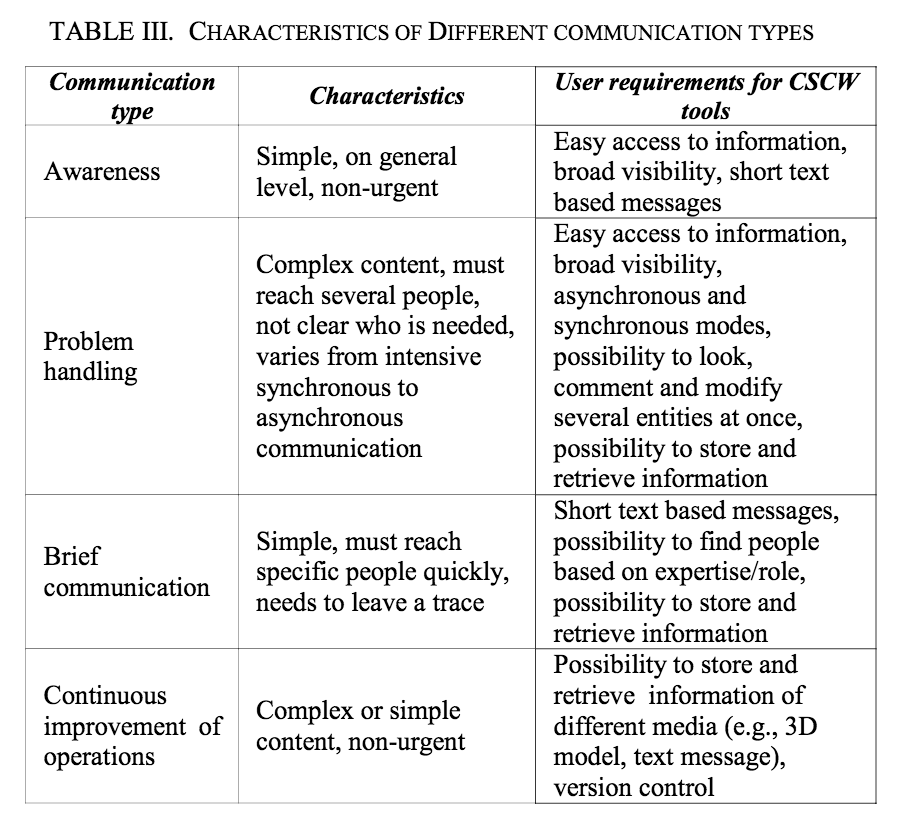
\includegraphics[width=.6\textwidth]{figures/Communication-types-table.png}
	\caption{Communication types}
	\label{comm_types}
\end{figure}

\textit{How designers think; the design process demystified}
(2nd ed. 1990)
by Bryan Lawson
\begin{itemize}
	\item Evolution of design:
	\begin{itemize}
		\item vernacular/ traditional design process
		\item cult of the individual (le Corbusier, Frank Lloyd Wright)
		\item ``collective control" (Jones), process forced to become more open to inspection and critical evaluation + scientific method
	\end{itemize}
	\item Jones' ``ultimate" definition of design: ``To initiate change in man-made things."
	\item Design process
	\begin{itemize}
		\item RIBA PoW is not a description of process, but of products of process
		\item ``It is about as much help in navigating a designer through his task as a diagram showing how to walk would be to a one year old child. [...] You will just have to put it all together for yourself." P. 28
	\end{itemize}
	\item Designing with others 
	\begin{itemize}
		\begin{figure}[htbp]
			\centering
			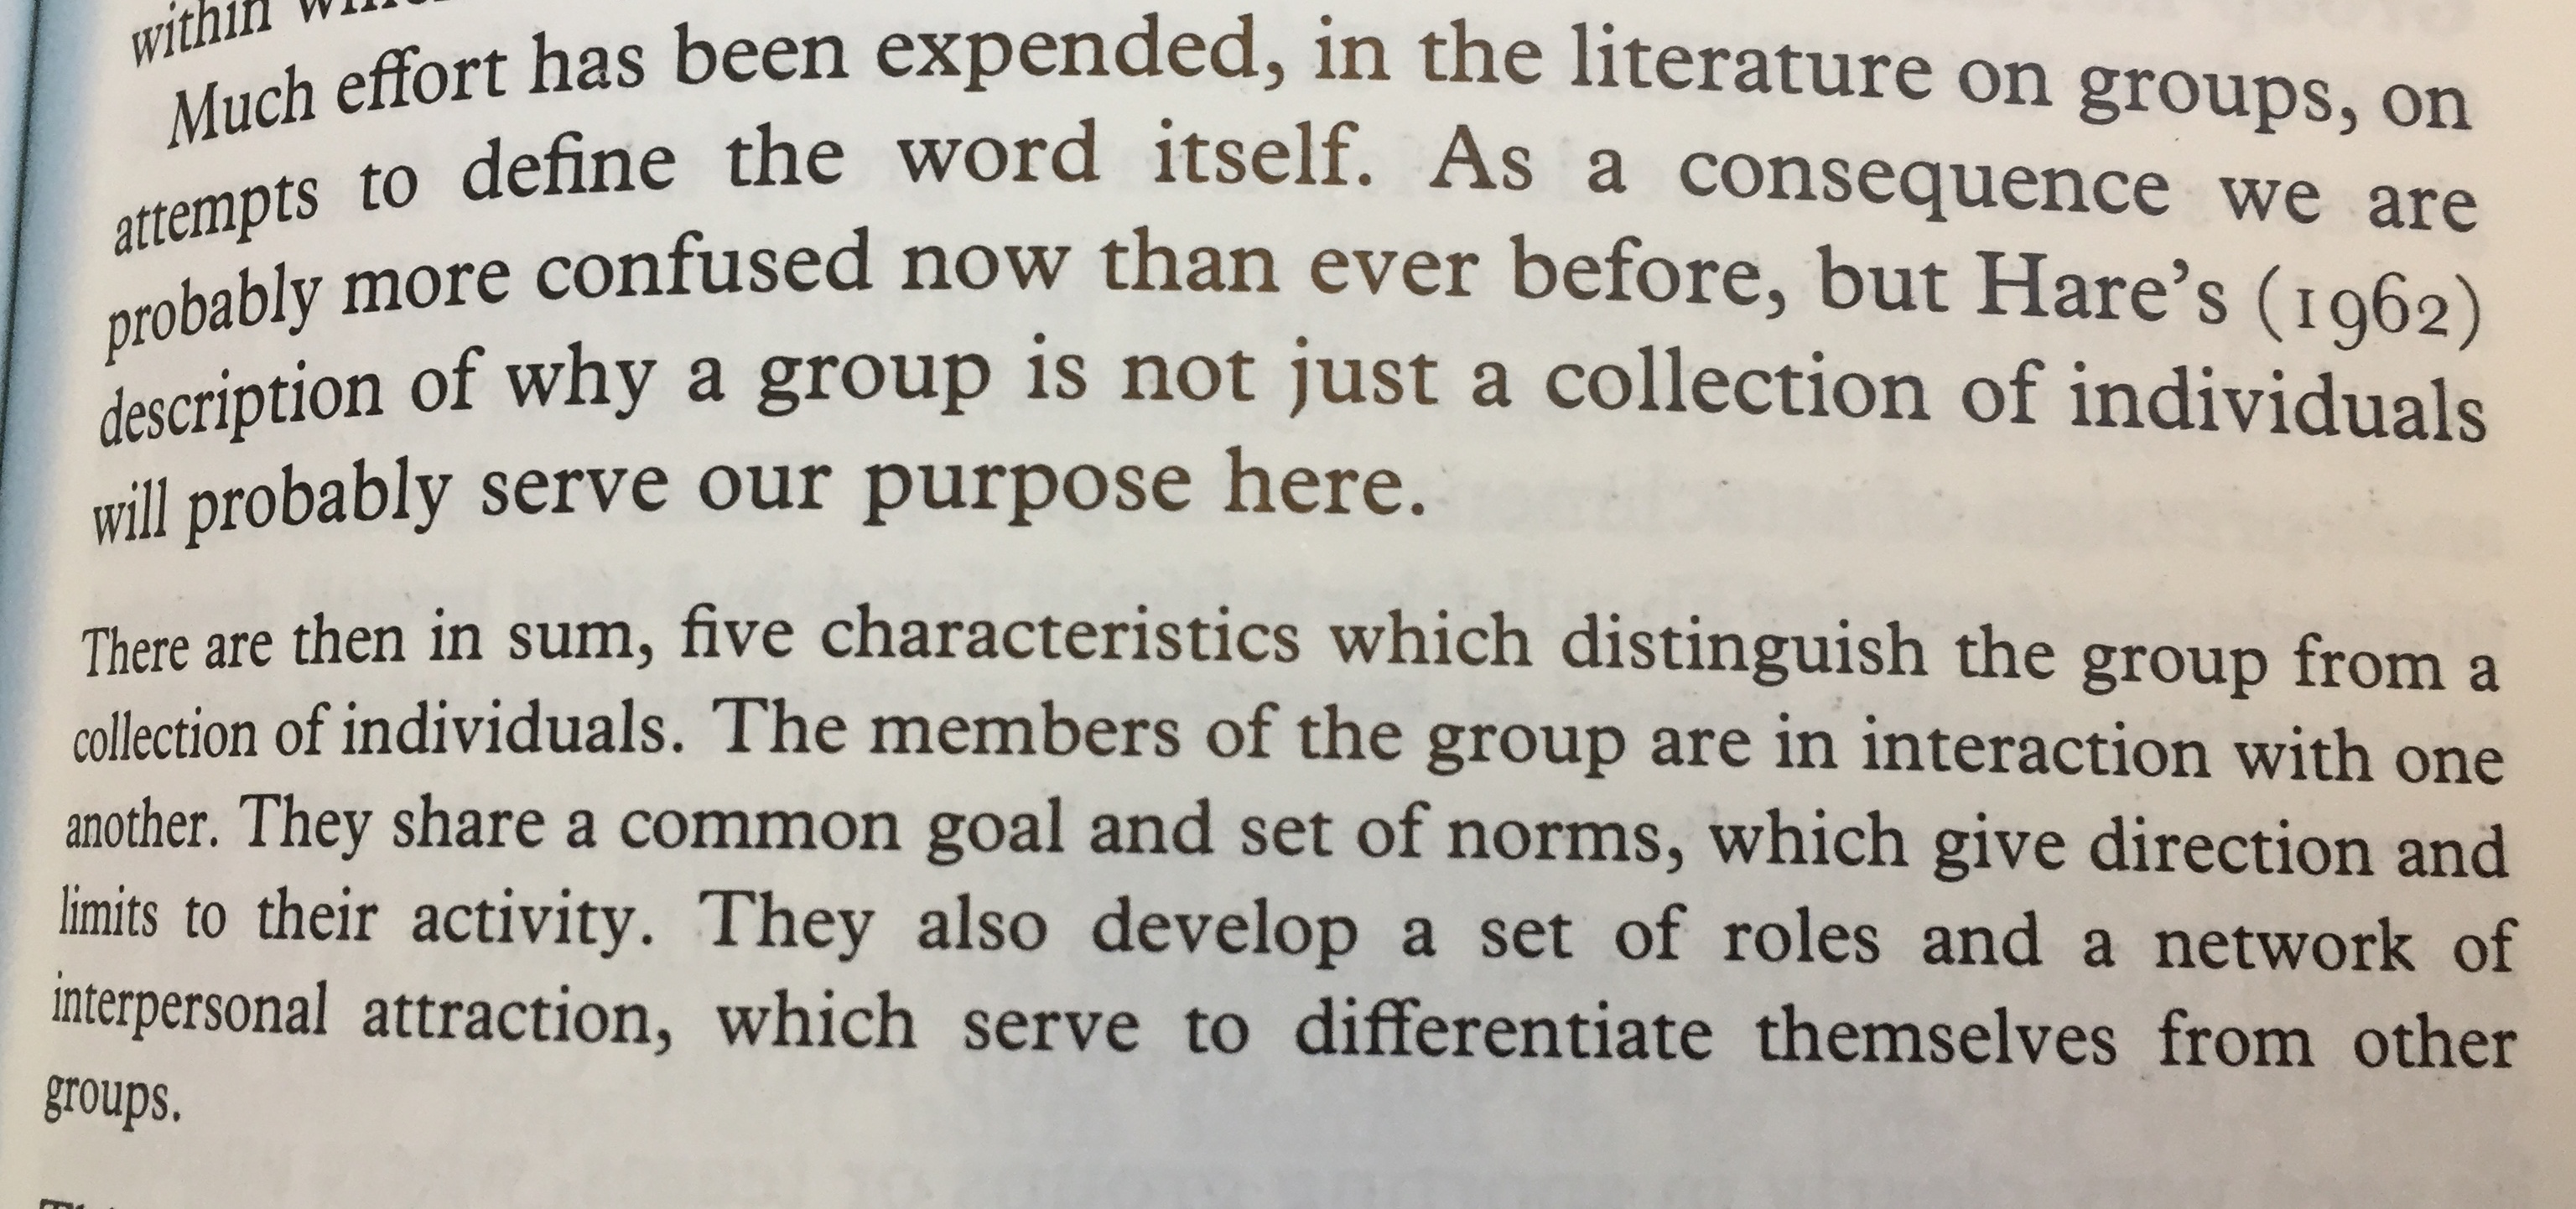
\includegraphics[width=.6\textwidth]{figures/Image.jpeg}
			\caption{Extract}
			\label{extract}
		\end{figure}
		\item Group vs. Collection of individuals - construction industry often acts as the latter? P. 189
		\item ``little has yet been written explicitly about design groups" p. 189
	\end{itemize}
\end{itemize}


\section{Interview}

	% title = {{MA PhD, Associate Professor at the School of Textiles \& Design at Heriot-Watt University}},

The purpose of the interview with Britta Kalkreuter was to find common language on describing communication in design.
This was to be done through hopefully drawing parallels between the construction and fashion industries.

Unfortunately, this comparative approach kind of backfired when I found out that Britta does not have much experience in fashion/ textiles.
She has a history in architectural history.
The courses she lectures at the School of Textiles and Design are primarily concerned with expression in the written word.
Her current research interests are in:
\begin{enumerate}
	\item Semantics and semiotics
	\item Design thinking and craft practice
	\item Heritage
\end{enumerate}
She described product semantics as \say{what a product communicates about itself or something else}.
My interests in communication might overlap with her interests in semantics and and design thinking.

The things we spoke about:
\begin{itemize}
	\item Design processes: crafts-based/ exploration of materials vs. designing for the end-user
	\item Modelling software
	\item Consultant/ contractor and designer/operator handover
	\begin{itemize}
		\item Communication breakdowns in designer/operator handovers
	\end{itemize}
	\item Communication 
	\begin{itemize}
		\item Her PhD student's paper - ``Craft and design interface", how negotiation occurs between craftsman and designer
		\item Communication types identified in Finnish journal article, particularly \say{continuous improvement of operations}
	\end{itemize}
\end{itemize}


%%%	EXCERPTS FROM INTERIM REPORT

The industry’s poor performance can largely be attributed to the its paradoxical nature; despite the in- dustry’s essence being intense collaborations on bespoke projects in temporary groupings (Laakso & Kiviniemi 2012), the industry is fragmented, with individual disciplines tending to work in isolation from others (IPA 2016, Miettinen & Paavola 2014).
--> WHY HAS COLLABORATION BEEN COUNTER-INTUITIVE TO CONSTRUCTION PROFESSIONALS WHEN IT IS REQUIRED?

The reports called for a reinvention of the AEC industry to improve its per- formance and put the client back in the centre. In order to achieve this, a need for collab- oration and standardisation was highlighted.
--> STDISATION FACILITATES/ ENABLES COLLABORATION

Amongst the government’s strategies for achieving this goal were enabling early contractor and supply chain involvement, standardising products and processes, and replacing adversarial cultures with collaborative ones. As part of the mobilisation towards collaboration, GCS 2011-15 required Building Information Modelling (BIM) Level 2 (explained in section 2.3) as a minimum on all public sector projects by 2016,
--> EARLY KOR INVOLVEMENT ALLOWS EARLIER COMMUNICATION + SMOOTHER HANDOVERS
--> IS THERE AN ADVERSARIAL CULTURE BETWEEN CIBSE AND TECHNICIANS/ WORKERS?
--> BIM INTRODUCED OUT OF NECESSITY FOR IMPROVED COLLABORATION

NBS (2014) defines BIM Level 2 as “distinguished by collaborative working –
all parties use their own 3D CAD models, but not necessarily working on a single, shared model. The collaboration comes in the form of how the information is exchanged between different parties – and is the crucial aspect of this level. Design information is shared through a common file format [such as IFC (Industry Foundation Classes) or COBie (Construction Operations Building Information Exchange)], which enables any organisation to be able to combine that data with their own in order to make a federated BIM model, and to carry
out interrogative checks on it.”
--> BIM LVL 2 DISTINGUISHED BY COLLABORATION THRU THE WAY INFO IS EXCHANGED (IFC, COBIE ETC.) --> DEFINITE BREAKDOWN IN COLLAB/ BIM LVL 2 WHEN IT COMES TO CONS TO KOR HANDOVER

\end{comment}

%----------------------------------------------------------------------------------------
%	INTRO
%----------------------------------------------------------------------------------------

% \hl{Alex: I would state that Egan, Latham, Collab4Change, even Farmer, all state collaboration / communication as a core issue and all as a positive contribution to effective performance. (Basically what you do at the start of Chapter 6)	That's enough.}

\cite{Latham1994}, \cite{Egan1998}, the government \citep{GCS11-15, GCS16-20} and \cite{Farmer2016} have all identified a lack of collaboration as being one of the great impediments to the effective performance of the AEC industry.
They have therefore asked AEC professionals to improve on their collaboration in order to deliver projects on time, on budget, and of good quality.
% The reports called for a reinvention of the AEC industry to improve its per- formance and put the client back in the centre. In order to achieve this, a need for collab- oration and standardisation was highlighted.
% So the industry/ government has asked the industry to get its sh*t/ act together and to start cooperating and collaborating better in order to provide better value, and reduce wastes in time and money.
This chapter will consider what is being asked of the industry by answering the following questions:
% Well, maybe we should delve into what is really being asked of the industry: 
\begin{enumerate}
	\item What is collaboration?
	% \item What does collaboration look like in the design and construction of a building?
	% \item Where and how does collaboration apply to building services engineers?
	\item What do collaboration and communication look like in the design and construction of a building?
	\item What are some failures in collaboration?
	% \item What should collaboration ideally look like in the setting…?
\end{enumerate}


%----------------------------------------------------------------------------------------
%	SECTION 1
%----------------------------------------------------------------------------------------

\section{What is Collaboration?}

\cite{collabor:oxford} defines collaboration as ``The action of working with someone to produce something".
\cite{wood1991toward} define collaboration as occurring ``when a group of autonomous stakeholders of a problem domain engage in an act or decide on issues related to that domain".
Further exploring the idea of a `group', according to \cite{hare1962handbook}, cited by \citeauthor{lawson1990} [\citeyear[p.~189]{lawson1990}], there are five characteristics that distinguish the group from a collection of individuals:
``The members of the group are [1] in interaction with one another.
They share [2] a common goal and [3] set of norms, which give direction and limits to their activity.
They also develop [4] a set of roles and [5] a network of interpersonal attraction, which serve to differentiate themselves from other groups."

Common traits that can be gathered from those three definitions are that collaboration is defined by:
\begin{itemize}
	\item Acting, deciding and/ or producing something %act, action, activity, decide, produce
	\item An interaction with at least one other person %with someone and group and interaction
	\item A shared problem and goal among the stakeholders %problem domain and common goal and set of norms
	\item The people involved each having an interest or concern in the problem or goal %autonomous roles
	\item The stakeholders being free to act independently
	\item The development of standard ways for the stakeholders to communicate with each other %and  (a person with an interest or concern in something (Oxford))
\end{itemize}



%----------------------------------------------------------------------------------------
%	SECTION 2
%----------------------------------------------------------------------------------------

\section{Collaboration and Communication in the Design and Construction of a Building}


%----------------------------
%	SUBSECTION 1
%----------------------------

\subsection{Where and How Does Collaboration Apply to Building Services Engineers?}

There are at least three different levels of communication and collaboration that building services engineers undergo during a project:
\begin{itemize}
	\item Discussion with the client/ employer about the end goal of the project (e.g. new build, refurbishment, expansion) and the issues related to achieving that goal.
	These times of discussion typically occur at the conceptual stage of a project and at planned checkpoints or meetings throughout the rest of the project.
	% Client/ employer, providing brief/ project requirements/ framework/ problem/ goal
	\item Communication and collaboration regarding the design and construction of the facility in the following settings:
	\begin{itemize}
		\item Discipline-external, i.e. with architects, structural engineers, project managers, quantity surveyors etc.
		\item Discipline-internal, i.e. with building services consultants and contractors etc.
	\end{itemize}
\end{itemize}

Processes, e.g. the RIBA PoW 2013, and contracts define the stages of a project and the required outputs of each stage.
It is important to note that processes such as the RIBA PoW 2013 are not prescriptive, but they merely provide a ``framework for the project team to approach design, construction and operational processes" \citep{Fairhead2015:online} by describing ``the products of the process" \citep{lawson1990}. % \hl{page number of quote} .
The reason for this is that the stakeholders, especially the designers, need freedom to act independently.
An analogy that explains designers' need of freedom from prescription is:
``It is about as much help in navigating a designer through his task as a diagram showing how to walk would be to a one year old child. [\ldots] You will just have to put it all together for yourself" \citep[p.~28]{lawson1990}.
Hence, one cannot say exactly when and with whom a building services engineer will collaborate; depending on the required outputs for each stage, building services engineers should seek collaboration with the appropriate people.
% Example: RIBA PoW 2013 “provides a framework for the project team to approach design, construction and opera- tional processes”
% + RIBA PoW is not a description of process (or is it?), but of products of process.


%----------------------------
%	SUBSECTION 2
%----------------------------

\subsection{Collaboration Patterns in Design}

% Despite this, it is worthy to note that t
The degree of collaboration between stakeholders on a design project has a typical pattern.
\cite{Parraguez2015} studied and identified patterns in the information flows between activities performed by stakeholders throughout the stages of complex engineering design projects.
They achieved this by analysing a ``large dataset collected from an industrial setting, consisting of project-related e-mails and activity records from the design and development of a renewable energy plant over the course of more than three years" \citep[p.~604]{Parraguez2015}.
They identified the stages of an engineering design process (see Figure \ref{fig_Parraguez_stages}) and three categories of design activities based on their functions.
``The first category includes activities related to the engineering design of specific components, modules, or subsystems under development; these we call modular subsystem activities.
The second category corresponds to activities with the objective of integrating two or more components, modules, or subsystems; these we call integrative subsystem activities.
A third category [\ldots] corresponds to activities that support, manage, and coordinate design work; for consistency, we call these integrative work activities" \citep[pp.~605--606]{Parraguez2015}.
% These three categories allow classifying activities based on their overall function and with this the means for aggregated analysis of information flows of each design stage."
The three categories allowed \citeauthor{Parraguez2015} to analyse the information flows between design activities  during each stage of the project.


\begin{figure}[tbp]
	\centering
	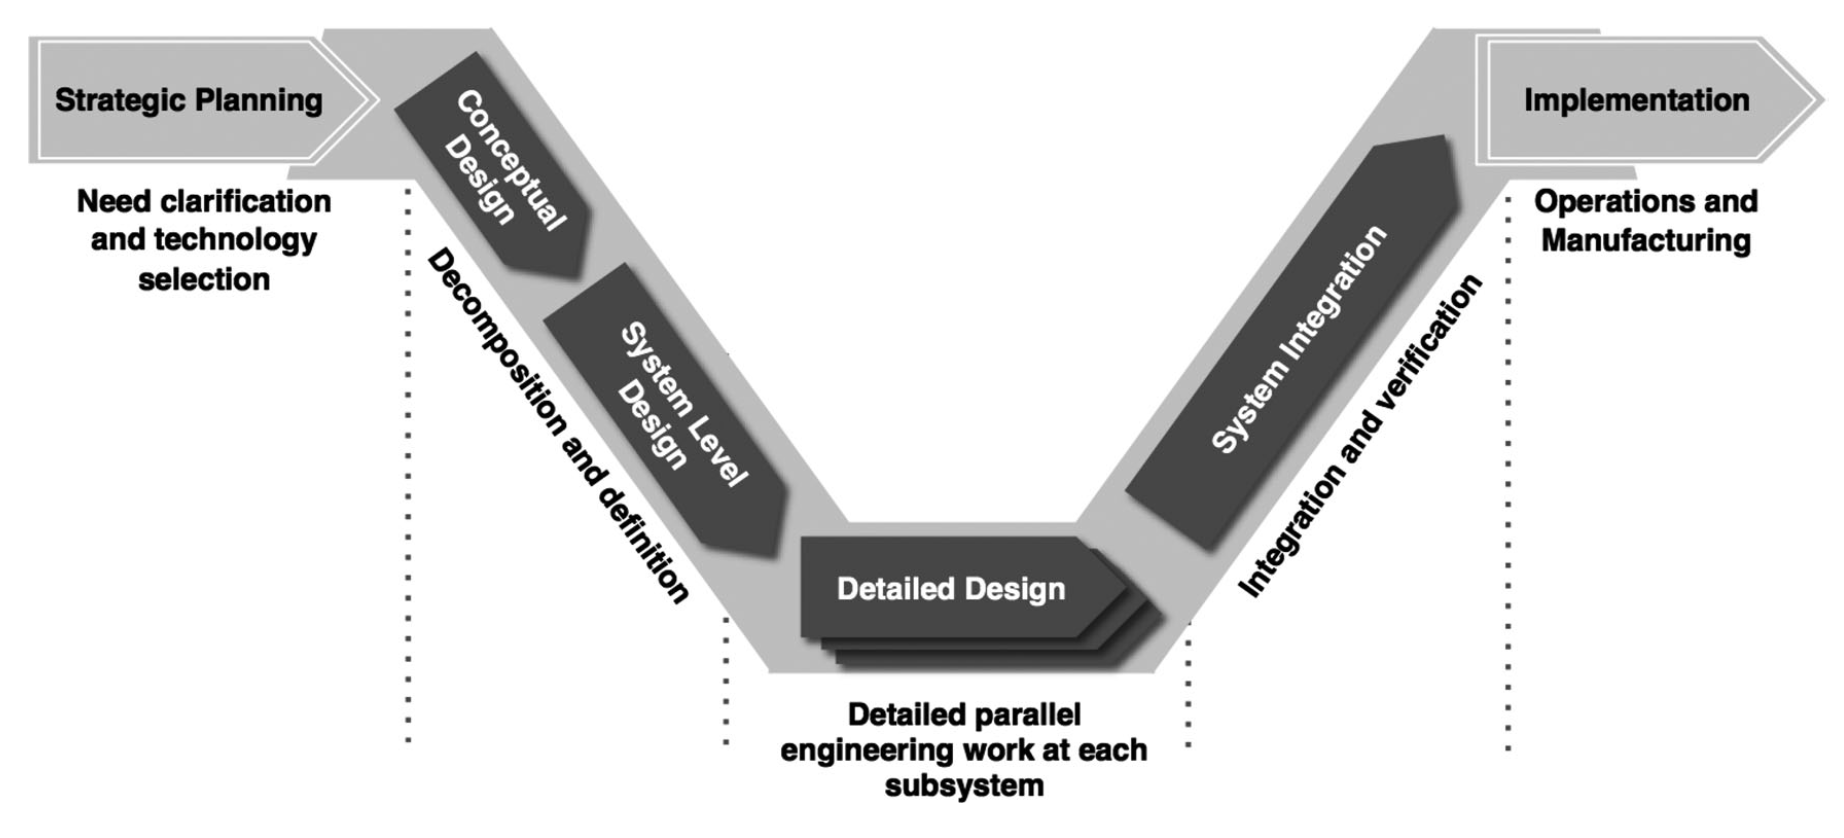
\includegraphics[width=\textwidth]{figures/Parraguez_stages.png}
	\rule{\textwidth}{0.5pt} % use line???
	\caption[Stages of the engineering design process.]{Stages of the engineering design process that can similarly apply to the stages of a building design process \citep[Figure~1]{Parraguez2015}.}
	\label{fig_Parraguez_stages}
\end{figure}


Figure \ref{fig_Parraguez_patterns} summarises their findings regarding the information patterns between activities for each stage.
% As illustrated in Figure \ref{fig_Parraguez_patterns} from \cite{Parraguez2015} who studied information flows in complex engineering design projects through activities and emails etc. (?).
It can be observed that there are strong information flows between and within most modular subsystem activities and integrative work activities at the Conceptual Design and System-Level Design stages.
However, at these early stages, the integrative subsystem activities and some of the modular subsystem activities have not yet established strong information flows within themselves.
At the Detailed Design stage, all of the activities have strong information flows within themselves, but there are weak information flows between the activities.
Lastly, at the System Integration stage, there are strong information flows within all activities and between most activities.
If the information flow patterns applied to the design process of a building, the findings of \cite{Parraguez2015} can be interpreted as follows:
\begin{enumerate}
	\item At the start of a project, there is strong collaboration between the client/ employer, designers and contractors in order to set and understand the brief; support, manage and coordinate the design work; and begin the individual design activities of the stakeholders.
	\item During the more detailed design stages, the stakeholders work mostly autonomously on modular subsystem activities with few interactions with each other.
	However, there might be strong collaboration between stakeholders on integrative subsystem activities.
	\item During the construction stage, there is strong collaboration between most activities.
\end{enumerate}

Regarding Stage 4 Technical Design, the RIBA PoW 2013 supports the second point:
``Using the design coordinated during the previous stage [i.e. Stage 3 Developed Design], the designers should now be able to develop their Technical Designs independently, with a degree of autonomy"
% The lead designer will provide input to certain aspects, including a review of each designer’s work" 
\citep{RIBAPlan}.


\begin{figure}[tbp]
	\centering
	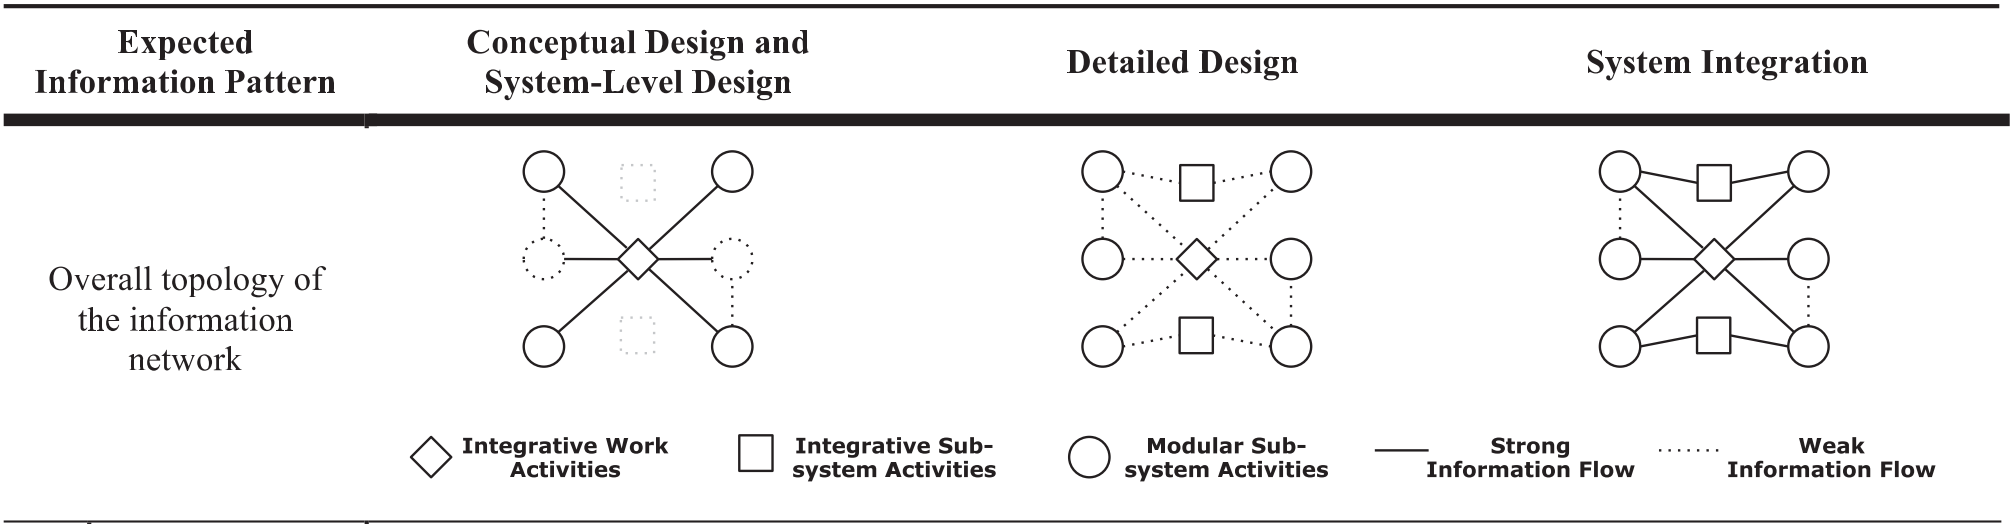
\includegraphics[width=\textwidth]{figures/Parraguez_patterns.png}
	\rule{\textwidth}{0.5pt} % use line???
	\caption[Information flow patterns between activities for each design stage.]{Information flow patterns between activities for each design stage \citep[Table~III]{Parraguez2015}.}
	\label{fig_Parraguez_patterns}
\end{figure}


%----------------------------
%	SUBSECTION 3
%----------------------------

\subsection{Communication Types in Design}

% \hl{Topic sentence.}
\cite{Holtta} studied and identified different types of communication regarding design content or design process in a buyer-supplier relationship within a product development network.
Additionally, \citeauthor{Holtta} highlighted characteristics of the design communication types that would facilitate the development of more effective communication tools.
They achieved this by studying the communication between a foundry\footnote{A foundry is a workshop or factory for casting metal \citep{foundry:oxford}.} and three of its customers, for whom the foundry manufactured components that were to be integrated with the customers' products.
A parallel could be drawn between this and the relationship that a product manufacturer or specialist designer has with a consultant.
Table \ref{table_communication_types} summarises their findings.
% \hlc{Create Latex table + explain then discuss findings (parallels to building design)}

% Please add the following required packages to your document preamble:
% \usepackage{booktabs}
\begin{table}[htbp]
\centering
\caption[Characteristics of different communication types.]{Characteristics of different communication types \citep[Table~III]{Holtta}. *CSCW: computer supported collaborative work.}
\label{table_communication_types}
\resizebox{\columnwidth}{!}{%
\begin{tabular}{@{}lll@{}}
	\toprule
	Communication type & Characteristics & User requirements for CSCW* tools \\ \midrule
	Awareness & \specialcell{l}{Simple, on general \\ level, non-urgent} & \specialcell{l}{Easy access to information, \\ broad visibility, short text \\ based messages} \\
	 & & \\
	Problem handling & \specialcell{l}{Complex content, must \\ reach several people, \\ not clear who is needed, \\varies from intensive \\ synchronous to \\asynchronous \\ communication} & \specialcell{l}{Easy access to information, \\ broad visibility, \\ asynchronous and \\ synchronous modes, \\ possibility to look, \\ comment and modify \\ several entities at once, \\ possibility to store and \\ retrieve information} \\
	 & & \\
	Brief communication & \specialcell{l}{Simple, must reach \\ specific people quickly, \\ needs to leave a trace} & \specialcell{l}{Short text based messages, \\ possibility to find people \\ based on expertise/ role, \\ possibility to store and \\ retrieve information} \\
	 & & \\
	\specialcell{l}{Continuous improvement \\ of operations} & \specialcell{l}{Complex or simple \\ content, non-urgent} & \specialcell{l}{Possibility to store and \\ retrieve information of \\ different media (e.g., 3D \\ model, text message), \\ version control} \\ \bottomrule
\end{tabular}
}
\end{table}


%----------------------------------------------------------------------------------------
%	SECTION 4
%----------------------------------------------------------------------------------------

\section{Communication \& Collaboration Failures}

% What are the weak points in collaboration/ why has the industry failed to collaborate so far/ why has collaboration been counter-intuitive to construction professionals when it is required?

Collaboration is often required in the AEC industry because the extent of a project can often exceed one's own knowledge and skill set.
However, information that is exchanged between multiple parties can be prone to distortion or even complete disappearance, such as in language translations and in the game \textit{Chinese Whispers}.

Communication failures seem to be a common problem when designing with others.
For example, in the fashion industry, labels that describe the materials used in an article of clothing are often inaccurate \citep{Kalkreuter2018}.
A designer may give a machine operator their design for a sweater in 100\% wool.
However the machine operator knows, through his practical craftsman skills, that it is impossible to weave wool in the way the designer has asked without adding nylon.
And so the machine operator adds nylon.
Along the way, the label may not get updated to state that the article contains both wool and nylon; instead, it states `100\% wool'.
This information may be left out accidentally or deliberately, perhaps because wool may be regarded as more valuable by the customer.
% \hl{listen to recording for jargon and re-write paragraph properly}.

% Common problem.
% Example: incorrect label problem during designer-manufacturer handover in textiles

% Idea of losing information during handovers, c.f. Chinese whispers, lost in translation?
% Can be researched further?
% Possible solution: minimise or eliminate handovers?
% Problem of skill set… Designer may not be able to manufacture and vice-versa.
% (That's the whole idea of collaboration and synergy, duh!)

% No regular meetings with client to understand goal.
% Famous chart where changes at the start are cheaper than changes towards the end of a project.
% Not fully understanding extent of project from outset.


%----------------------------------------------------------------------------------------
%	SECTION 5
%----------------------------------------------------------------------------------------

% \section{Conclusion/ Summary}

\chapter{Tools and Interoperability} % Main chapter title

\label{Chapter7} % Change X to a consecutive number; for referencing this chapter elsewhere, use \ref{ChapterX}

\lhead{Chapter 7. \emph{Tools and Interoperability}} % Change X to a consecutive number; this is for the header on each page - perhaps a shortened title

%----------------------------------------------------------------------------------------
%	SECTION 1
%----------------------------------------------------------------------------------------

% Solibri…
% Include other ``tools/ technologies" as they are called by Fred, e.g. IFC, COBie (?)?
% Revit.
% Bluebeam Revu.

\section{BIM Software Providers}

The market-leading BIM software providers are Autodesk, Bentley, Nemetschek, and Trimble \citep{Bosche, BusinessWire}.
The most commonly used software programme for building services engineers in the UK is Autodesk Revit MEP.

%----------------------------------------------------------------------------------------
%	SECTION 2
%----------------------------------------------------------------------------------------


\section{Problems of Interoperability}
% Part of the root of these problems is the lack of interoperability due to weakly coordinated market demand for standards e.g. IFC.
Interoperability is the ability of different software applications to exchange and make use of data \citep{Gallaher2004}.
The benefit of interoperability is illustrated in Figure \ref{io}. If no common open standard exists, each individual software application must develop and implement direct translators back and forth for all other pieces of software which it seeks to communicate with. If an open standard can be used instead, the mappings only need to be translated back and forth from that single format in order to be compatible with all other applications supporting the same standard \citep{Laakso2012}.
\cite{Laakso2012} explain that it might seem natural for a user to adopt an open format, considering its theoretical benefits.
But, as an anecdotal example shows, this is not always the case.
Free and open word processing software applications have been available for several years, and yet the Microsoft Word file format (a vendor-specific proprietary format) continues to be perceived as the de-facto standard format.

\begin{figure}[htbp]
	\centering
	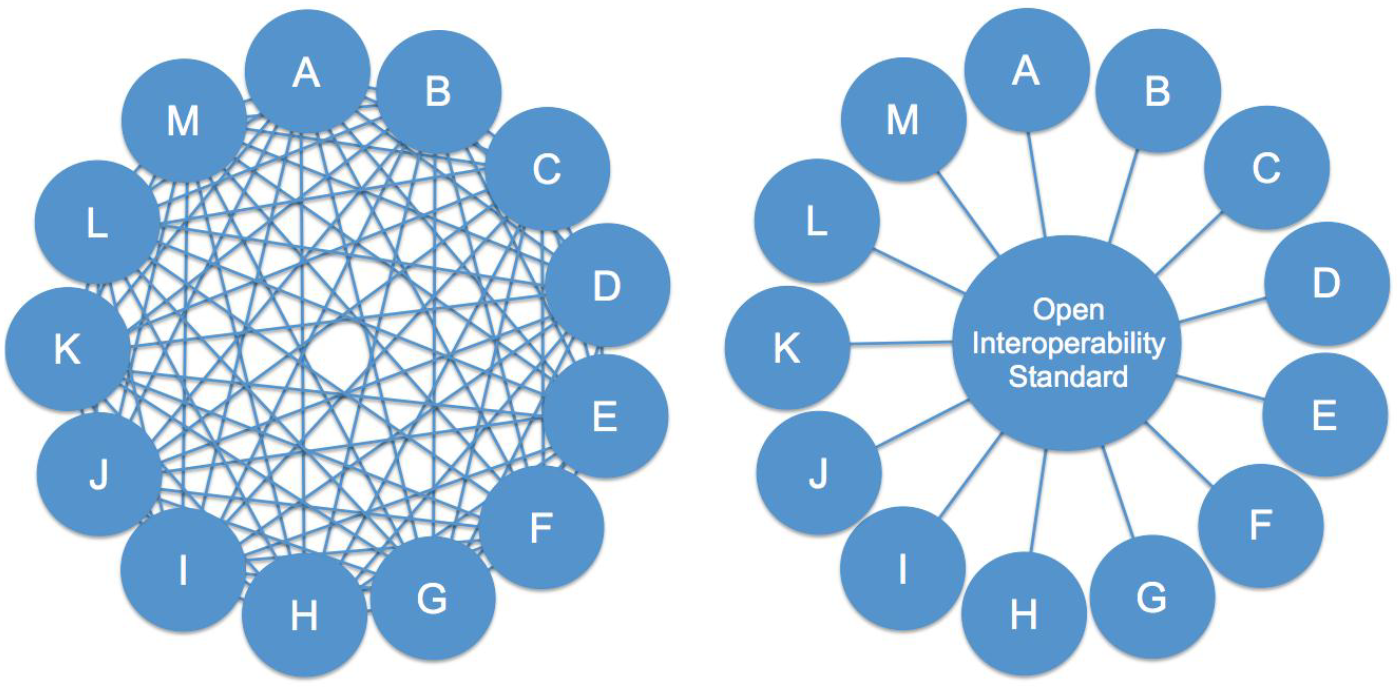
\includegraphics[width=\textwidth]{figures/Interoperability.png}
	\rule{\textwidth}{0.5pt} % use line???
	\caption[Direct translators between software applications vs. an open interoperability standard]{Direct translators between software applications vs. an open interoperability standard \citep{Laakso2012}.}
	\label{io}
\end{figure}

The Industry Foundation Classes (IFC) are an open, internationally recognised and standardised data model that is intended to enable interoperability between BIM software applications \citep{Laakso2012}.
The origins of IFC date back to the early 1990s \citep{Laakso2012}.
Considering that the first BIM software to be made available on a personal computer was released in 1984 \citep{Quirk2012}, IFC developed relatively early.
According to \cite{Laakso2012}, buildingSMART (the developer of IFC) wished to standardise IFC during the early stages of BIM so that IFC could be implemented into the new BIM software applications entering the marketplace, thus preventing proprietary solutions from gaining dominance.
This plan unfortunately did not work specifically due to the low market demand for BIM technologies in the early stages, thus making it challenging to get sufficient resources to manage the development of the IFC standard.
As a result, the exchange of BIM data has been dominated by proprietary solutions.
Moreover, although IFC has been around for a relatively long time and even been implemented into leading BIM software, actual use of IFC as an enabler of interoperability has been slow but steadily increasing \citep{Laakso2012}.

\chapter{Industry Guidance on Collaboration Processes} % Main chapter title

\label{Chapter8} % Change X to a consecutive number; for referencing this chapter elsewhere, use \ref{ChapterX}

\lhead{Chapter 8. \emph{Industry Guidance}} % Change X to a consecutive number; this is for the header on each page - perhaps a shortened title

%----------------------------------------------------------------------------------------
%	CHAPTER INTRO
%----------------------------------------------------------------------------------------

This chapter summarises some of the guidance that is provided by the industry and government for the collaboration of building services engineers.

%----------------------------------------------------------------------------------------
%	SECTION 1
%----------------------------------------------------------------------------------------

\section{Authoritative Documents}

There is a myriad of documents published by the AEC industry and the government that provide guidance on how construction professionals should communicate and collaborate with each other.
This especially since a call for collaboration was made in the Latham and Egan Reports, and the Cabinet Office mandated BIM Level 2 on public sector projects in 2011.
Some of the main guides that concern building services engineers and that have been analysed for the purposes of this thesis are displayed in red on the timeline in Figure \ref{timeline}.
%The documents that dictate the processes of work (i.e. activities and deliverables for every work stage) or building services engineers are displayed in \hl{red} in the timeline in figure \ref{timeline}.
Most of the guides are aligned with the RIBA PoW 2013, except for PAS 1192-2 which aligns itself with the CIC Scope of Services stages.
However, the CIC Scope of Services stages are more or less aligned with RIBA PoW 2013, as shown in Figure \ref{fig_pow_alignments}.
The purpose and content of the main guides are outlined below:
\begin{itemize}
    \item \textbf{PAS 1192-2:2013} \citep{PAS1192}: A standard that provides guidance for information requirements, generation and flow using BIM during the capital expenditure (CAPEX) phase of construction projects.
    \item \textbf{BG 6} \citep{BG62014}: 
    %Provides an \say{aide-memoire of design activities, first where this clarifies the duties listed in standard forms of agreement for appointing design consultants, and second where allocation of design activity is either currently overlooked or is open to debate.} // 
    %This is the building services engineer’s `bible' that provides guidance on their activities, and drawing and model definitions for each stage of the design and construction process. // 
    A technical guide that provides a framework for allocating many of the design activities, in connection with the building services aspects of a construction project, to the different members of a project team. It provides standard pro-formas, as well as exemplary drawings and models for each stage of a project.
    \item \textbf{CIBSE Digital Engineering (DE) Series} [\citeauthor{DE2}, 2016-17]: A series of documents that provide practical guidance for the full built environment supply chain (not just building services engineers) on how to deliver a project using BIM.
    \item \textbf{ACE Schedule of Services; MEP} \citep{ACE2017}: A document that sets out the services to be performed by MEP engineers on projects.
\end{itemize}


\begin{figure}[htbp]
	\centering
	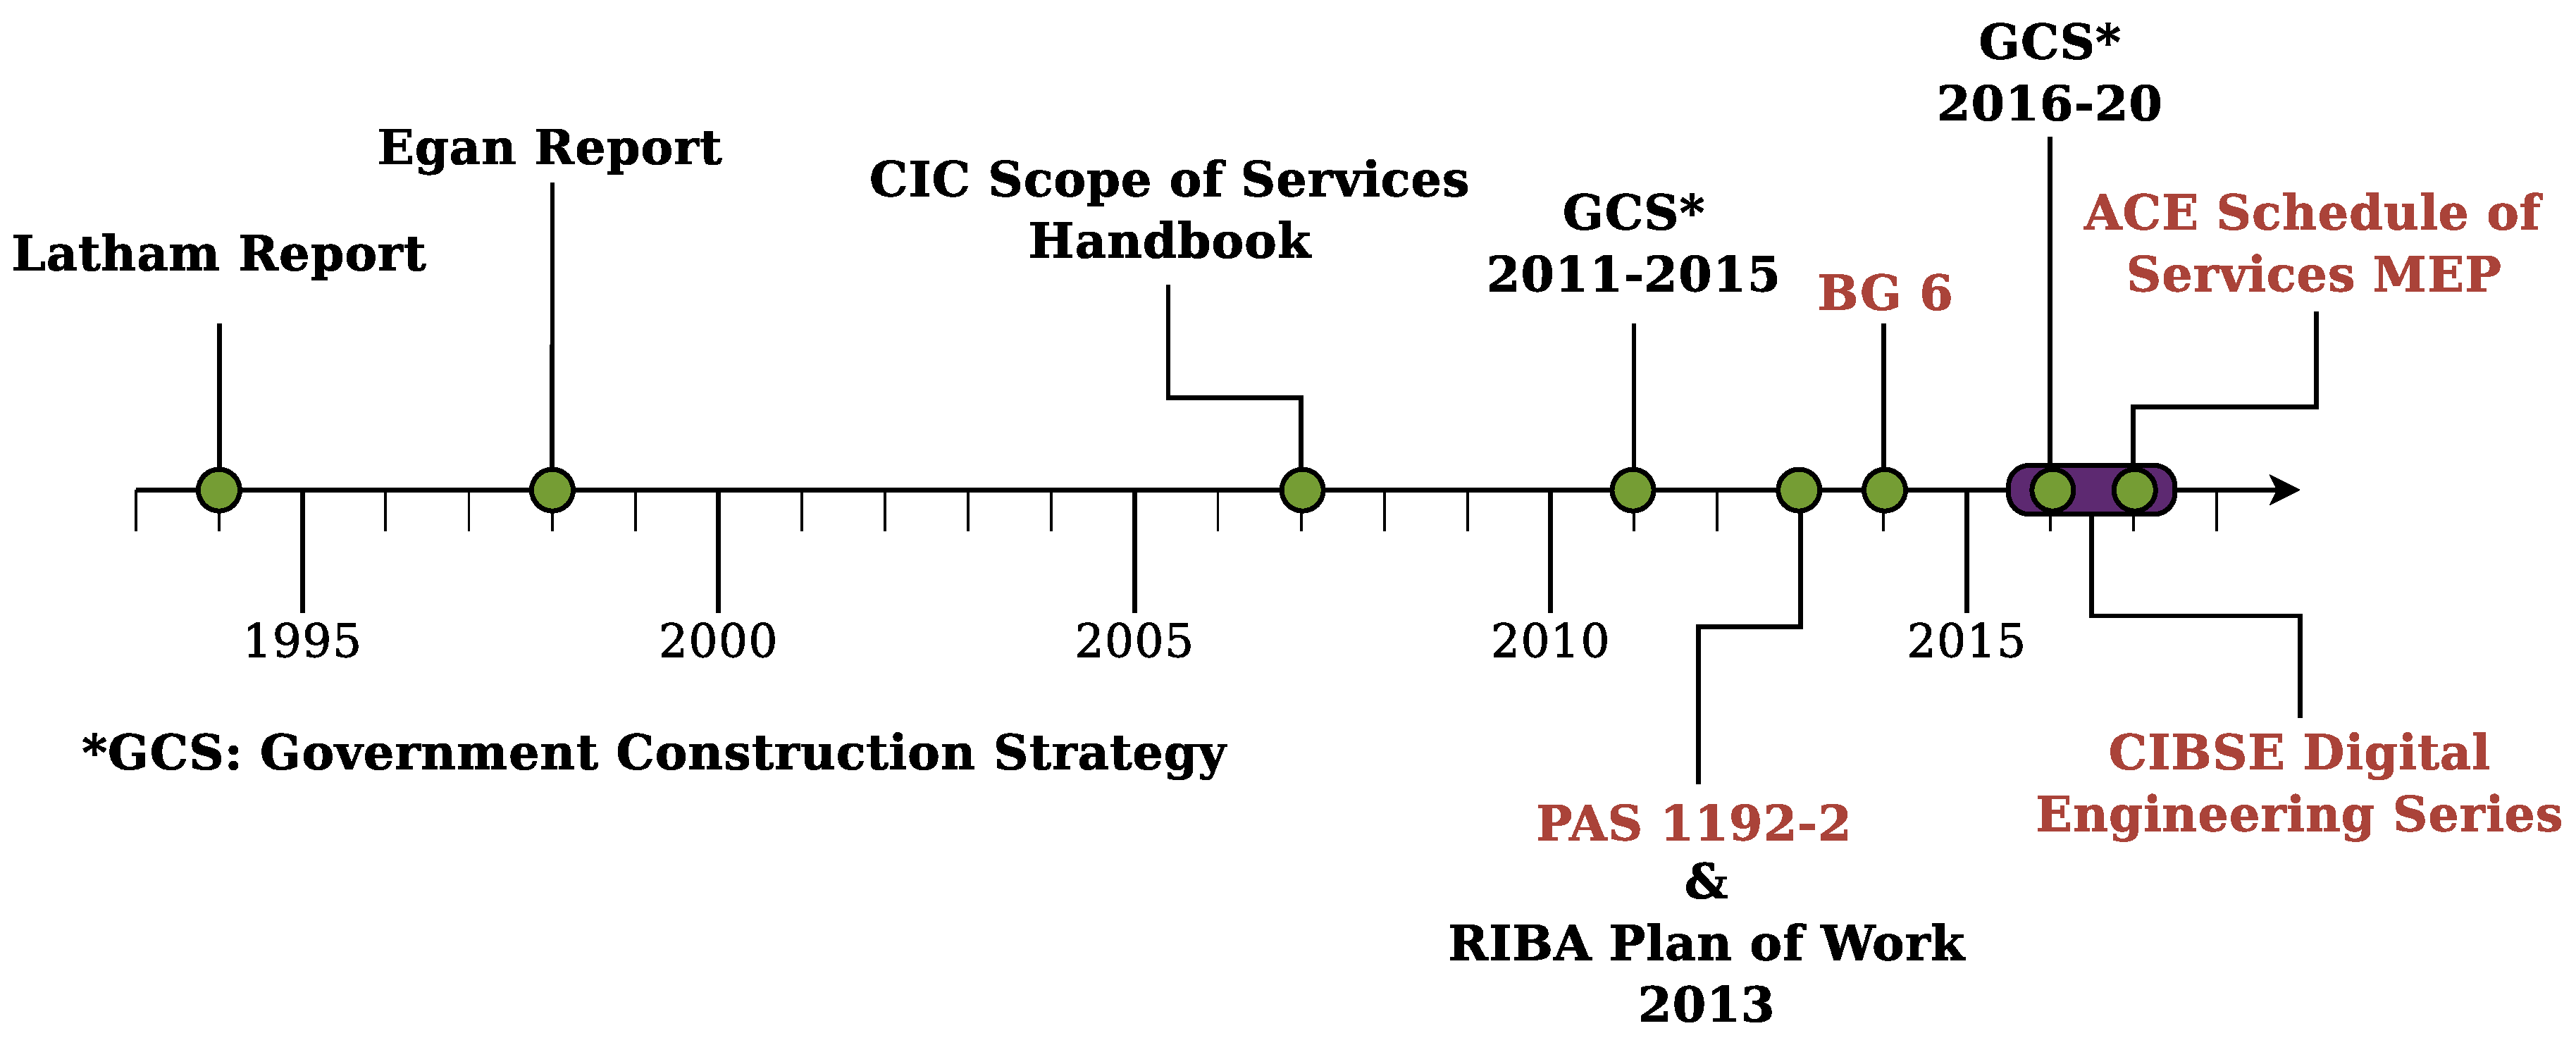
\includegraphics[width=\textwidth]{figures/Timeline2.eps}
	\rule{\textwidth}{0.5pt} % use line???
	\caption[Timeline of government construction strategies, and industry reports and guides since 1994.]{Timeline of government construction strategies, and industry reports and guides since 1994. The main guides that concern building services engineers are displayed in red.}
	\label{timeline}
\end{figure}


\begin{figure}[htbp]
	\centering
	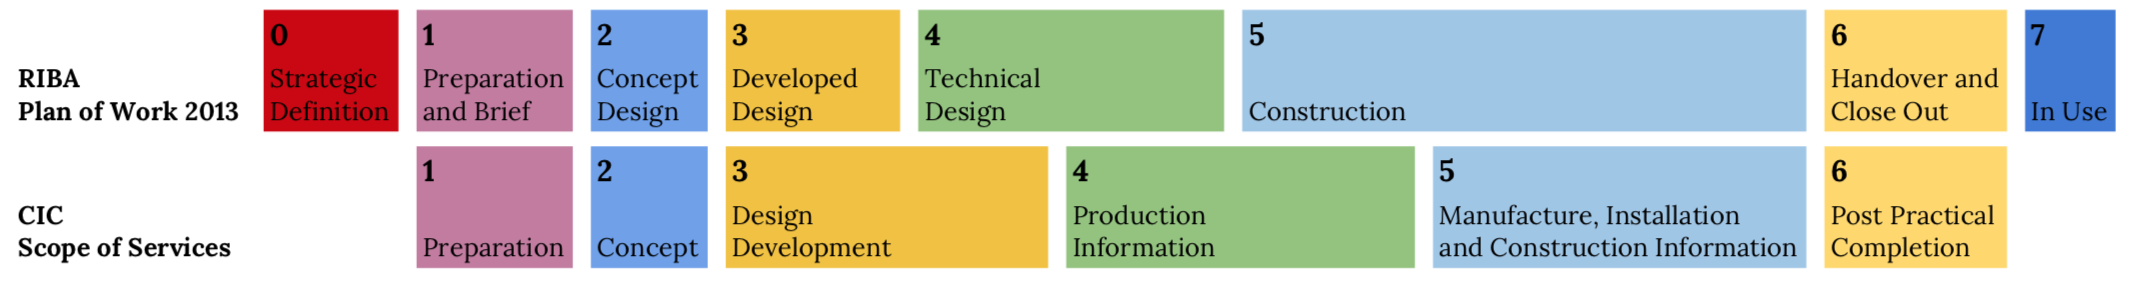
\includegraphics[width=\textwidth]{figures/PoW_Alignments.png}
	\rule{\textwidth}{0.5pt} % use line???
	\caption[Alignment of RIBA PoW 2013 and CIC Scope of Services stages]{Alignment of RIBA PoW 2013 and CIC Scope of Services stages \citep{CIC2007, ArchitectsJournal}.}
	\label{fig_pow_alignments}
\end{figure}


The following two sections summarise the main findings regarding the collaboration of building services engineers regarding consultant-to-contractor handovers and levels of definition.



\begin{comment}
\textbf{What did I find out?}
The documents, although a bit messy and not speaking exactly the same language or using exactly the same PoW, were more in agreement than I expected.
They all admit to the flexibility required for building services engineers during Stage 4. In fact, they state that contractors can intervene at even earlier stages of the process. 
Despite this (when the consultants/ contractors are in charge), the activities/ deliverables/ services remain the same.
\end{comment}


%----------------------------------------------------------------------------------------
%	SECTION 2
%----------------------------------------------------------------------------------------

\section{Consultant-to-Contractor Handover Points}

The AEC industry seems to agree on the necessity for flexibility
regarding the handover points between building services consultants and contractors \citep{BG62014, ACE2017, CIC2007, RIBAPlan}.
The handover points vary according to the selected procurement routes, as exemplified in Figure \ref{fig_BG6_handover_pts}.
The BG 6 \citep{BG62014}, ACE Schedule of Services \citep{ACE2017} and RIBA PoW 2013 \citep{RIBAPlan} stress on the importance of understanding the selected procurement route and clarifying the allocation of responsibilities between the consultant and contractor at an early stage.
According to \cite{RIBAPlan}, ``The Design Responsibility Matrix \footnote{A Design Responsibility Matrix is a \say{matrix that sets out who is responsible for designing each aspect of the project and when. [\ldots] The Design Responsibility Matrix is created at a strategic level at Stage 1 and fine tuned in response to the Concept Design at the end of Stage 2 in order to ensure that there are no design responsibility ambiguities at Stages 3, 4 and 5.} \citep{RIBAPlan}} sets out how these key design interfaces will be managed."
%According to \cite{ACE2017}, ``The Stage at which a contractor may be engaged will influence decisions made in this respect."
%The ACE SoS and B1M \hl{and BIM?} stress on the importance of clarifying the times of the handover points from the outset of a project.
%According to \hl{some people, B1M and CIBSE DES?}, the handover points should be stated in the \hl{BIM Execution Plan and Master Information Delivery Plan}.

\begin{figure}[htbp]
	\centering
	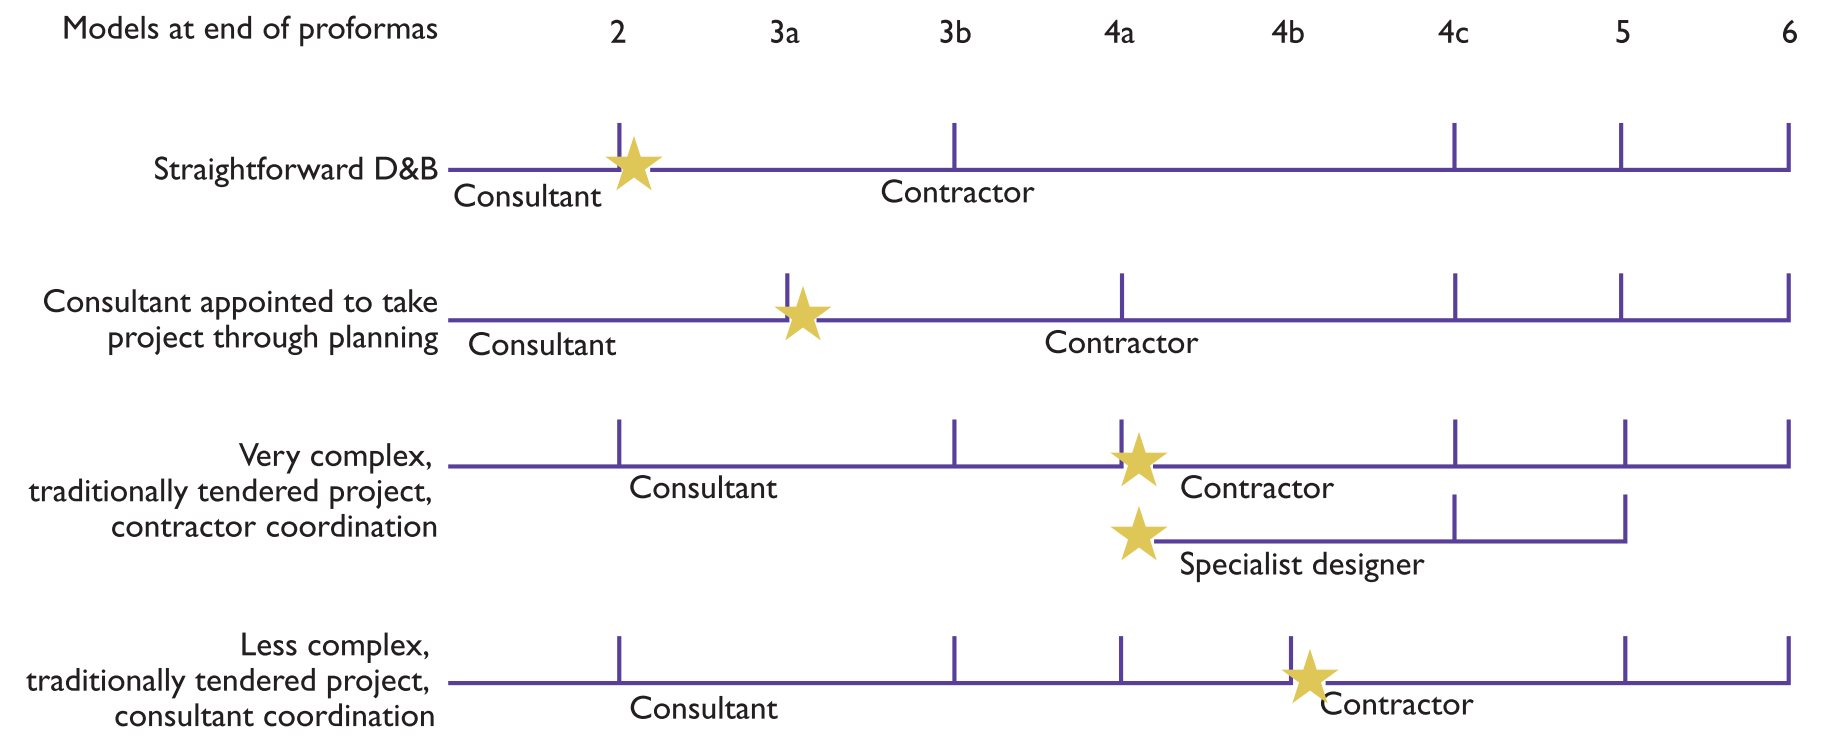
\includegraphics[width=\textwidth]{figures/BG6_handover_pts.png}
	\rule{\textwidth}{0.5pt} % use line???
	\caption[Potential handover points between consultant, contractor and specialist designers.]{``Some potential handover points between consultant, contractor and specialist designers [\ldots]. The vertical lines indicate when models might be produced and the [stars] represent handover from one organisation to another. But these examples are neither prescriptive nor exhaustive." \citep[p.~2]{BG62014} (Figure borrowed and slightly adapted from BG 6.)}
	\label{fig_BG6_handover_pts}
\end{figure}


%----------------------------------------------------------------------------------------
%	SECTION 3
%----------------------------------------------------------------------------------------

\section{Levels of Definition} \label{section:LODs}

% What most of these documents boiled down to (explicitly or implicitly) were the levels of definition.

%------------------------------
%	DEFINITION
%------------------------------

The term `level of definition' is defined in PAS 1192-2 \citep{PAS1192} as the collective term for two specific areas of information:
\begin{itemize}
	\item Level of model detail: ``the description of graphical content of models at each of the stages defined for example in the CIC Scope of Services"
	\item Level of model information: ``the description of non-graphical content of models at each of the stages defined, for example, in the CIC Scope of Services"
\end{itemize}

%------------------------------
%	ACRONYMS
%------------------------------

The industry uses the acronym LOD to represent several terms. 
In the UK, LOD is more commonly used to describe the `level of definition', but LOD has also been used to represent the `level of detail' or `level of design' \citep{Fairhead2015:book}.
In the USA, LOD stands for `level of development' \citep{BIMForum2017}.
However, within the context of this thesis, the following acronyms shall be used, unless otherwise stated:
\begin{itemize}
	\item LOD: level of definition
	\item LoD: level of model detail
	\item LoI: level of model information
\end{itemize}

%------------------------------
%	SUBSECTION 1: WHY LODS WERE INTRODUCED
%------------------------------

\subsection{Origin and Purpose of LODs}

According to \cite{Fairhead2015:book}, ``LOD is an acronym developed primarily in support of BIM data".
In an NBS article, \cite{NBS_LoD_Kell} explains that ``Following the Government `Level 2' BIM mandate [\ldots] the need for the project team overall to provide consistent digital information at an equivalent level across design stages" arose and implies that LODs were the solution for this.
Therefore, LODs serve as a tool ``to improve the quality of communication among users of Building Information Models (BIMs) about the characteristics of elements in models" \citep{BIMForum2017}.

The industry is generally recommended to define the LODs for each work stage early on in a project so that they are understood by all relevant members of the project team.
This is similar to the emphasis the industry places on clarifying the consultant-to-contractor handover points 
Table \ref{clarify_LODs} shows a sample of sources and the project documents in which they recommend setting the LODs.
Among these sources is The B1M, the self-proclaimed ``definitive video channel for construction".
As can be seen in Table \ref{clarify_LODs}, the recommendations vary from source to source.
However, all of the recommended project documents are supposed to be created at the start of a project.
Therefore, the sources are in agreement with respect to establishing the LODs from the outset of a project.

% Please add the following required packages to your document preamble:
% \usepackage{booktabs}
\begin{table}[htbp]
\centering
\caption[Project documents in which it is recommended to set the LODs.]{A sample of sources and the project documents in which they recommend setting the LODs.}
\label{clarify_LODs}
\resizebox{\columnwidth}{!}{%
\begin{tabular}{@{}lcccccc@{}}
\toprule
	 & CIC BIM Protocol & EIR$^1$ & BEP$^2$ & MIDP$^3$ & DRM$^4$ & Design Programme \\ \midrule
	\specialcell{l}{PAS 1192-2 \\ \citep{PAS1192}} & \checkmark & \checkmark & \checkmark &  &  &  \\
	 & & & & & & \\
	\specialcell{l}{CIBSE DE2: EIR \\ \citep{DE2}} &  & \checkmark &  &  &  &  \\
	 & & & & & & \\
	\specialcell{l}{The B1M \\ \citep{B1M_LODs_explained}} &  &  & \checkmark & \checkmark &  &  \\
	 & & & & & & \\
	\specialcell{l}{RIBA Plan of Work 2013 \\ \citep{RIBAPlan}} &  &  &  &  & \checkmark & \checkmark \\ \bottomrule
	\multicolumn{7}{l}{\textit{$^1$ Employer's Information Requirements \hspace{2em} $^2$ BIM Execution Plan}} \\
	\multicolumn{7}{l}{\textit{$^3$ Master Information Delivery Plan \hspace{3em} $^4$ Design Responsibility Matrix}} \\
\end{tabular}
}
\end{table}

%------------------------------
%	SUBSECTION 2: IDEA VS SPECIFIC TERMS
%------------------------------

\subsection{Unclear Use of Phrase ``Level of Detail"}

All of the studied guidance documents use the exact phrase ``level of detail" at least once. % \citep{DE2, RIBAPlan, ACE2017, CIC2007, PAS1192, BG62014}.
However, the use of the phrase can be somewhat confusing.
It is not always clear whether the documents are referring strictly to the term LoD, i.e. the description of graphical content of models, or if they are referring to the idea of `an extent of information or detail of something' in a graphical or non-graphical format.
Table \ref{unclear_LoD} summarises the author's interpretations of the documents' intentions when they use the phrase ``level of detail".
In Table \ref{unclear_LoD}, it can be observed that after PAS 1192-2 defined LoD, only the second publication of the CIBSE DE series (DE2: EIR) strictly uses the phrase ``level of detail" to refer to LoD.
There are instances in the ACE Schedule of Services MEP when the use of ``level of detail" is unclear and when it clearly refers to LoD.
The use of ``level of detail" in BG 6 is never clear.
%The documents that clearly refer to the terms LoD and LoI are PAS 1192-2 \citep{PAS1192}, CIBSE DE2, ACE Schedule of Services MEP.
%As for the BG 6 and RIBA PoW 2013, it is not always clear whether the official terms are being referred to.
%The CIC Scope of Services cannot refer to the official definitions because it was published before the PAS 1192-2.

% Please add the following required packages to your document preamble:
% \usepackage{booktabs}
\begin{table}[htbp]
\centering
\caption[Use of the phrase ``level of detail" in guidance documents.]{Author's interpretations of the guidance documents' intentions when they use the phrase ``level of detail".}
\label{unclear_LoD}
\resizebox{\columnwidth}{!}{%
\begin{tabular}{@{}llll@{}}
	\toprule
	& LoD & Idea & Intention unclear \\
	Documents & \specialcell{l}{Graphical content \\ of model} & \specialcell{l}{Extent of information \\ or detail of something} & \specialcell{l}{Could mean either \\ LoD or idea} \\ \midrule
	\specialcell{l}{CIC Scope of Services Handbook \\ \citep{CIC2007}} &  & \checkmark * &  \\
	 & & & \\
	\specialcell{l}{PAS 1192-2 \\ \citep{PAS1192}} & \checkmark &  &  \\
	 & & & \\
	\specialcell{l}{BG 6 \\ \citep{BG62014}} &  &  & \checkmark \\
	 & & & \\
	\specialcell{l}{ACE Schedule of Services MEP \\ \citep{ACE2017}} & \checkmark &  & \checkmark \\
	 & & & \\
	\specialcell{l}{CIBSE DE2: EIR \\ \citep{DE2}} & \checkmark &  &  \\ \bottomrule
	\multicolumn{4}{l}{\textit{*Published before LoD was defined in PAS 1192-2}} \\
\end{tabular}
}
\end{table}

%------------------------------
%	SUBSECTION 3: COMMON INDUSTRY STDS
%------------------------------

\subsection{Recognised Interpretations of LODs}

The author has identified three recognised interpretations of LODs that apply to building services engineers.
The interpretations are displayed in Table \ref{LODs}, which also shows some organisations that endorse their use.

% Please add the following required packages to your document preamble:
% \usepackage{booktabs}
\begin{table}[htbp]
\centering
\caption[Recognised interpretations of LODs and their endorsements.]{Recognised interpretations of LODs and the organisations that endorse their use.}
\label{LODs}
\resizebox{\columnwidth}{!}{%
\begin{tabular}{@{}llll@{}}
\toprule
& AIA & BSRIA & NBS \\
Organisation & \specialcell{l}{Levels of \\ Development} & \specialcell{l}{BG 6 Model Definitions \\ and Drawing Definitions} & \specialcell{l}{NBS BIM Toolkit Levels of Detail \\ and Levels of Information} \\ \midrule
\cite{CIC2007} &  & \checkmark * &  \\
 & & & \\
NBS \citep{NBS_LODs} & \checkmark & \checkmark & \checkmark \\
 & & & \\
CIBSE \citep{DE2} &  & \checkmark & \checkmark \\
 & & & \\
\cite{ACE2017} & \checkmark &  & \checkmark \\ \bottomrule
\multicolumn{4}{l}{\textit{*Endorses 1$^{st}$ edition of BG 6 published in 2006 \citep{BG62006}}} \\
\end{tabular}
}
\end{table}

%------------------------------
%	SUBSECTION 4: WORK STAGE RELATED
%------------------------------

\subsection{Are LODs Related to Work Stages?}

The numbers of the aforementioned LODs create the impression that they are related to the work stages (see Table \ref{LOD_stage_alignment}).
However, there appears to be a disagreement in the industry on whether LODs are work stage related or not.

PAS 1192-2, BSRIA's BG 6 and NBS seem to associate LODs with work stages in the following ways:
\begin{itemize}
	\item The definitions for LoD and LoI in PAS 1192-2  (see definitions at start of Section \ref{section:LODs}) are linked with work stages, as is illustrated in Figure \ref{PAS_RIBAPoW_alignment}.
	
	\item The BG 6 aligns its pro-formas with the RIBA PoW 2013 (see Figure \ref{BG6_RIBAPoW_alignment}).
	Each pro-forma defines the model and drawing definitions (i.e. the BG 6's LODs) for the associated stage of the project.
	Additionally, illustrative examples of the model and drawing definitions are interleaved with the pro-formas, as shown in Figures \ref{fig_BG6_MD4a} and \ref{fig_BG6_DD4a}.
	
	\item Figure \ref{NBS_LoD_alignment} from NBS shows that their BIM Toolkit LoDs are representative of the work stages.
	Furthermore, \cite{NBS_LoD_Kell} says in an NBS article that the RIBA PoW 2013 ``workstages and necessary outputs define the intended level of detail to be delivered by each design discipline".
\end{itemize}


In contrast, the ACE Schedule of Services MEP and CIBSE DE2 seem to imply that LODs are not strictly related to work stages in the following ways:
\begin{itemize}
	\item In CIBSE DE2, \cite{DE2} argues, ``The BIM Task Group guidance note suggests that [the defining of LoDs and LoIs] can be done as a blanket value for the whole project, changing at each project stage; this is actually not possible, as different aspects of a project progress at different speeds. For example, the structure will be more progressed than the lighting design at concept stage."
		
	\item The ACE Schedule of Services MEP provides ``Typical examples of the levels of development of information to be provided for Stages 2–4 in line with the core Deliverables" in its appendix \citep{ACE2017}.
	Some of the prescribed LODs in these examples do not correlate with the work stage number, as seen in Table \ref{ACE_st3_LODs}.
\end{itemize}

PAS 1192-2, BG 6 and the NBS article were respectively published in 2013, 2014 and 2015, whereas CIBSE DE2 and the ACE Schedule of Services MEP were respectively published in 2016 and 2017.
There appears to be a correlation between the publication dates of these documents and their guidance on whether LODs are work stage related.
Perhaps this suggests that the industry realised in 2016 that LODs should not be work stage related.
%However, this is purely speculation made without any firm evidence.
More recent publications by BSI, BSRIA and NBS might confirm this speculation.


\begin{figure}[htbp]
	\centering
	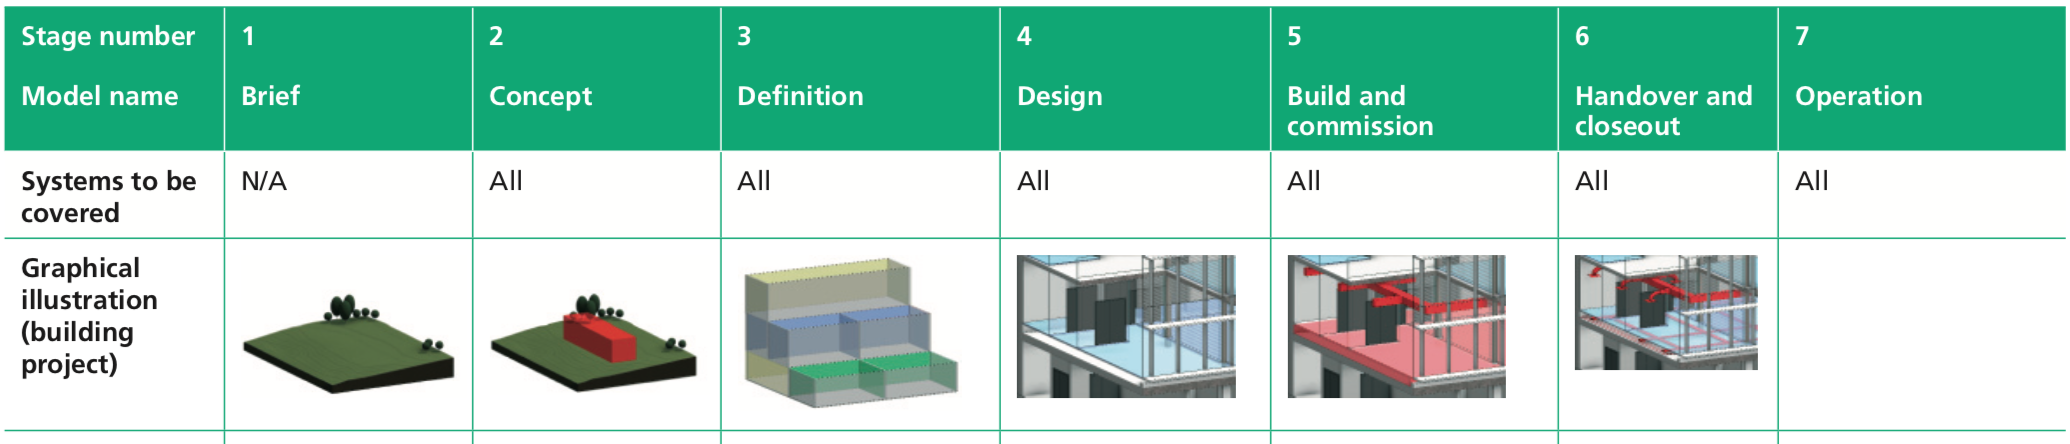
\includegraphics[width=\textwidth]{figures/PAS_RIBAPoW_alignment.png}
	\rule{\textwidth}{0.5pt} % use line???
	\caption[Alignment of work stages with PAS 1192-2 LODs.]{Extract from PAS 1192-2 showing alignment of CIC Scope of Services stages with levels of model definition for building projects \citep[Figure~20]{PAS1192}}
	\label{PAS_RIBAPoW_alignment}
\end{figure}


\begin{figure}[htbp]
	\centering
	\begin{subfigure}[b]{.25\textwidth}
		\centering
		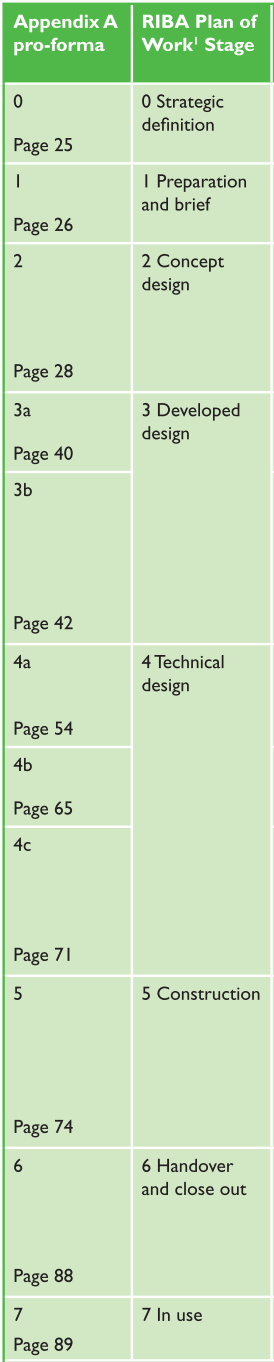
\includegraphics[width=\textwidth]{figures/BG6_RIBAPoW_alignment.png}
		\rule{\textwidth}{0.5pt} % use line???
		\caption{BG 6}
		\label{BG6_RIBAPoW_alignment}
	\end{subfigure}%
	\begin{subfigure}[b]{.75\textwidth}
		\centering
		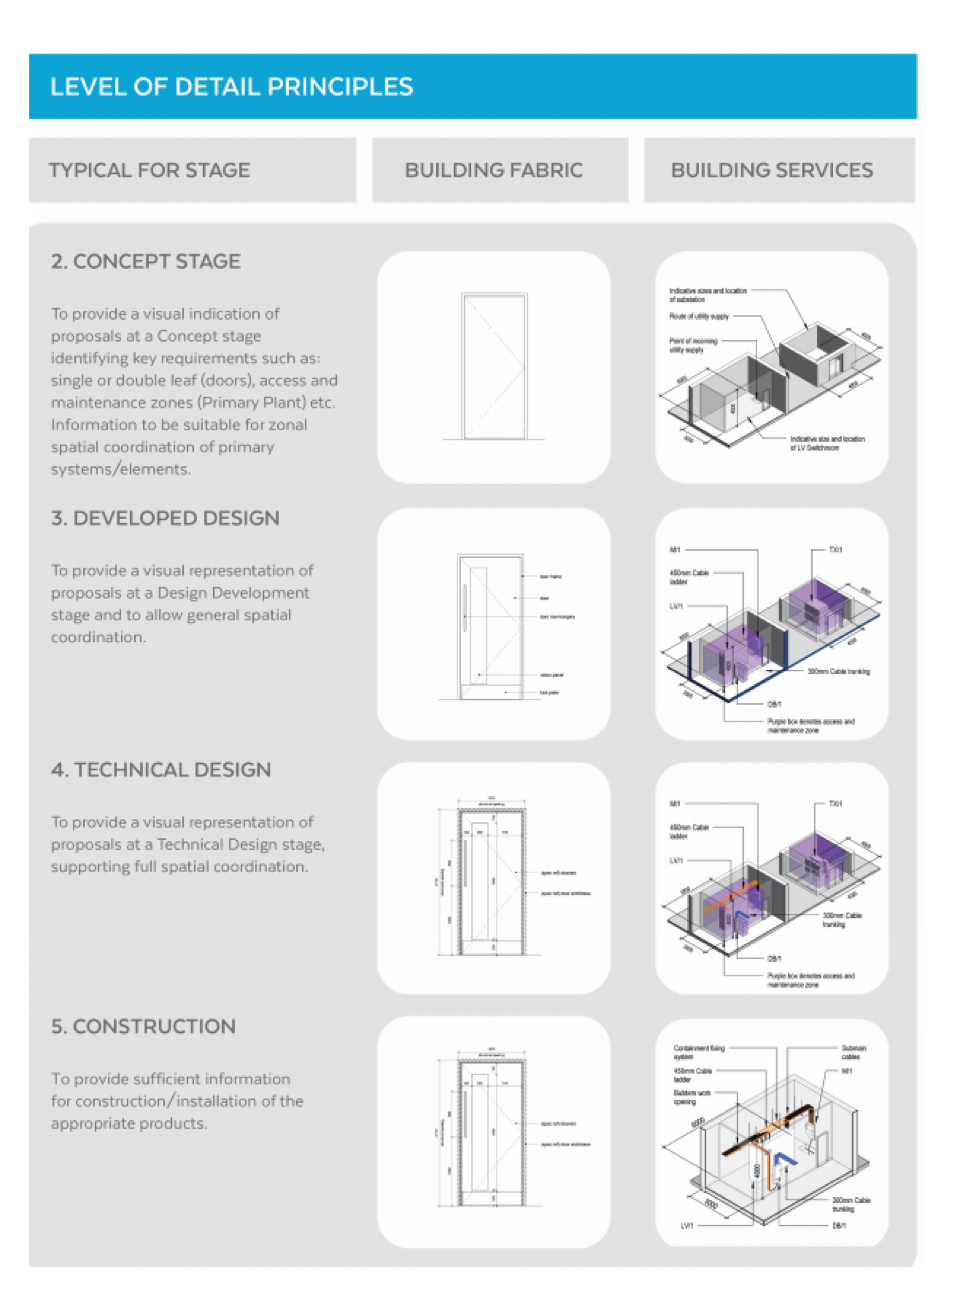
\includegraphics[width=\textwidth]{figures/NBS_LoD_alignment.png}
		\rule{.93\textwidth}{0.5pt} % use line???
		\caption{An example of NBS BIM Toolkit LoDs}
		\label{NBS_LoD_alignment}
	\end{subfigure}
	\caption[Alignment of work stages with BG 6 and NBS LODs.]{Alignment of RIBA PoW 2013 stages with ({\scriptsize A}) BG 6 pro-formas \citep[Table~1]{BG62014} and ({\scriptsize B}) NBS BIM Toolkit's LoDs \citep{NBS_LoD_Kell}.}
	\label{BG6_NBS_alignment_w_stages}
\end{figure}


\begin{figure}[htbp]
	\centering
	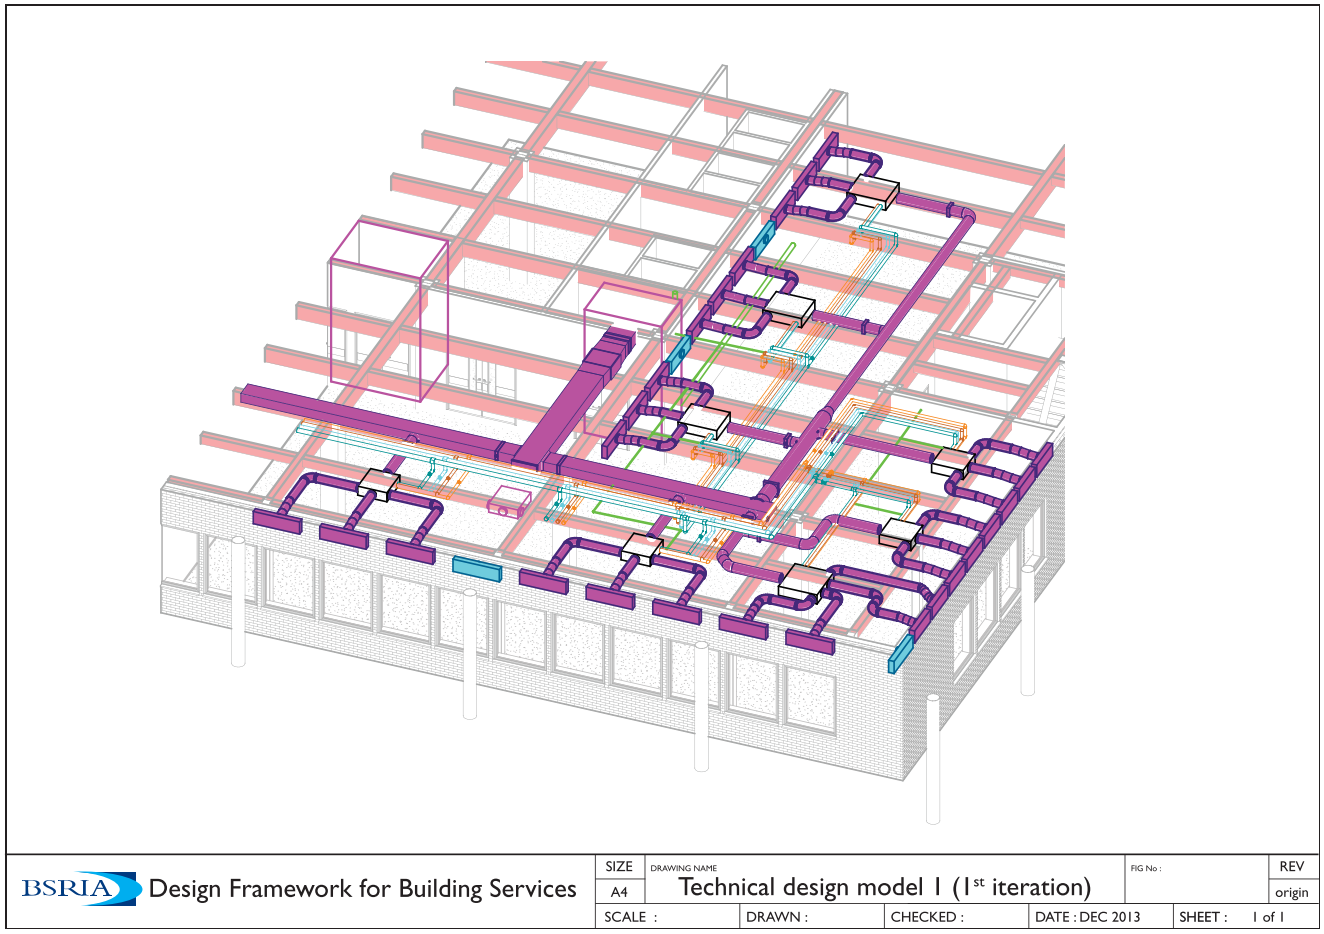
\includegraphics[height=.4\textheight]{figures/BG6_MD4a.png}
	\rule{.9\textwidth}{0.5pt} % use line???
	\caption[One of BG 6's model definitions for Stage 4a.]{One of BG 6's model definitions for Stage 4a \citep{BG62014}.}
	\label{fig_BG6_MD4a}
\end{figure}


\begin{figure}[htbp]
	\centering
	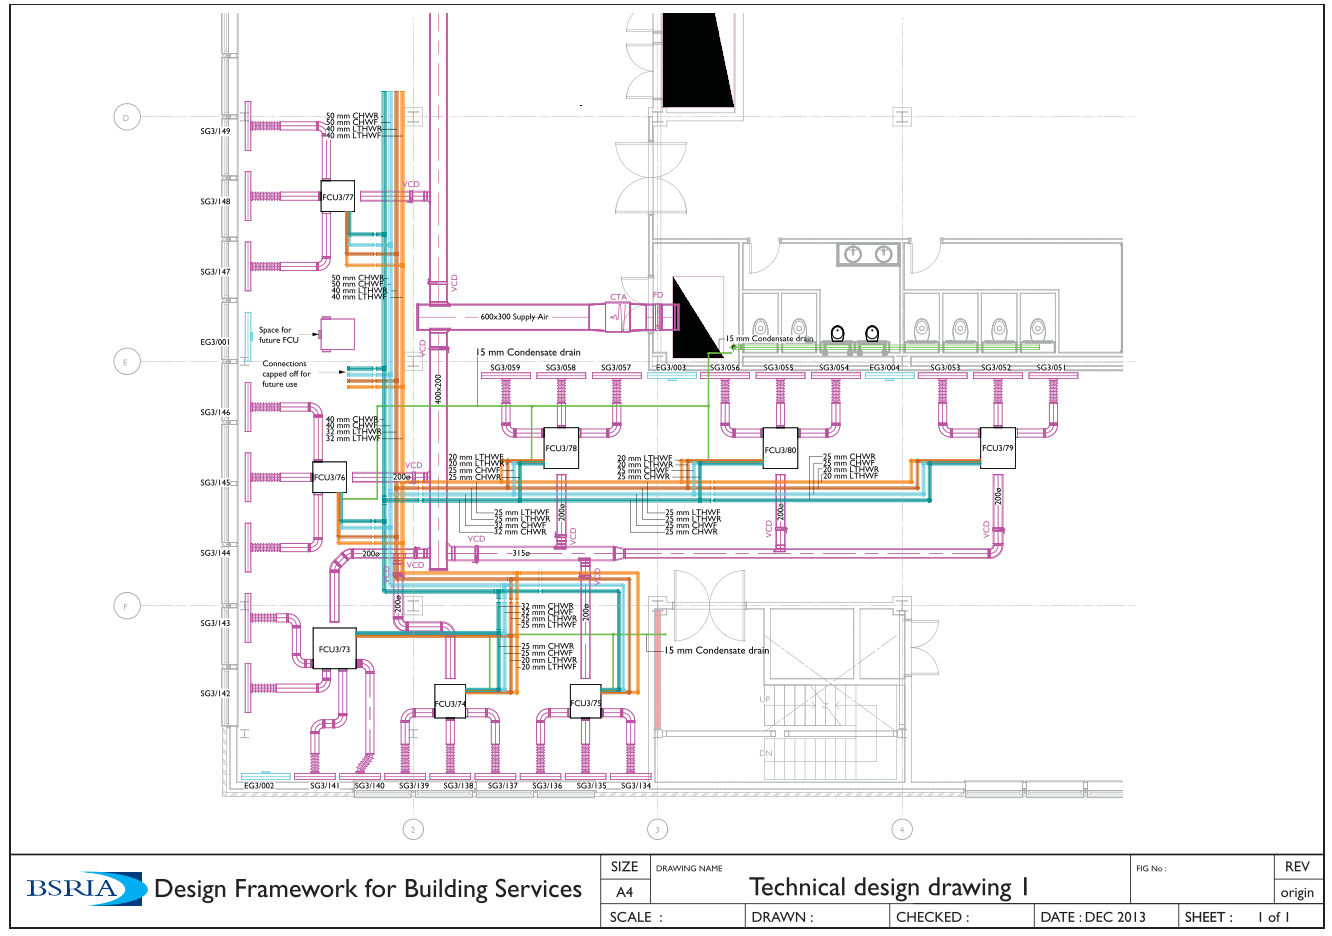
\includegraphics[height=.4\textheight]{figures/BG6_DD4a.png}
	\rule{.9\textwidth}{0.5pt} % use line???
	\caption[One of BG 6's drawing definitions for Stage 4a.]{One of BG 6's drawing definitions for Stage 4a \citep{BG62014}.}
	\label{fig_BG6_DD4a}
\end{figure}


% Please add the following required packages to your document preamble:
% \usepackage{booktabs}
\begin{table}[htbp]
\centering
\caption[Numbers of LODs and their resemblant alignment with the work stages.]{Numbers of recognised interpretations of LODs and their resemblant alignment with the work stages of the RIBA Plan of Work 2013 and CIC Scope of Services. (N.B. In reality, the LODs might not be aligned to the work stages in this way or in any way.)}
\label{LOD_stage_alignment}
\resizebox{\columnwidth}{!}{%
\begin{tabular}{@{}lllll@{}}
	\toprule
	RIBA Plan of Work 2013 & \multicolumn{3}{l}{Levels of Definition} & CIC Scope of Services \\ \cmidrule(lr){2-4}
	Stages & AIA$^{\dagger}$ & BG 6* & NBS BIM Toolkit$^{\ddagger}$ & Stages \\ \midrule
	0 Strategic Definition &  & 0 &  &  \\
	1 Preparation and Brief & LOD 100 & 1 &  & 1 Preparation \\
	2 Concept Design & LOD 200 & 2 & 2 Concept Stage & 2 Concept \\
	3 Developed Design & LOD 300 & 3a & 3 Developed Design & 3 Design Development \\
	& LOD 350 & 3b &  &  \\
	4 Technical Design & LOD 400 & 4a & 4 Technical Design & 4 Production Information \\
	&  & 4b &  &  \\
	&  & 4c &  &  \\
	5 Construction & LOD 500 & 5 & 5 Construction & 5 Manufacture, Installation \\
	&  &  &  & and Construction Information \\
	6 Handover and Close Out &  & 6 &  & 6 Post Practical Completion \\
	7 In Use &  & 7 &  &  \\ \bottomrule
	\multicolumn{5}{l}{\textit{$^{\dagger}$LOD in this column stands for ``Level of Development".}} \\
	\multicolumn{5}{l}{\textit{*The numbers refer to the BG 6 pro-formas which, amongst other things, describe the levels of}} \\
	\multicolumn{5}{l}{\textit{graphical information required in models and drawings.}} \\
	\multicolumn{5}{l}{\textit{$^{\ddagger}$NBS does correlate its LoDs as being ``Typical for Stage [\ldots]" \citep[Figure~3]{NBS_LoD_Kell}}} \\
\end{tabular}
}
\end{table}

% Please add the following required packages to your document preamble:
% \usepackage{booktabs}
\begin{table}[htbp]
\centering
\caption[Typical example of the LODs to be provided for Stage 3.]{Typical example of the LODs to be provided for RIBA Plan of Work Stage 3 (table borrowed and slightly adapted from \cite{ACE2017}).}
\label{ACE_st3_LODs}
\resizebox{\columnwidth}{!}{%
\begin{tabular}{@{}lllll@{}}
\toprule
	 & \specialcell{l}{NBS BIM \\ Toolkit \\ LoD} & \specialcell{l}{NBS BIM \\ Toolkit \\ LoI} & \specialcell{l}{AIA LOD$^{\dagger}$} & Notes \\ \midrule
	Primary equipment & 2 & 2 & LOD200 & \specialcell{l}{Major plant equipment \\ modelled as generic objects.} \\
	 & & & & \\
	Secondary equipment & N/A & N/A & Typical details only & \specialcell{l}{Typical details shown (e.g. \\ fan coil unit connections), \\ but not modelled in \\every space.} \\
	 & & & & \\
	Primary Distribution & 2 & 2 & LOD200 & \specialcell{l}{Primary distribution \\ routes modelled for all \\ services. Spatial allowance \\ proven for insulation, \\ accessories and fittings.} \\
	 & & & & \\
	Secondary Distribution & 1 & 1 & LOD100 & \specialcell{l}{Spatial allowance proven \\ for secondary pipework \\ and ductwork \\ distribution} \\
	 & & & & \\
	Terminal Units & 2 (typical only) & 2 (typical only) & LOD200 (typical only) & \specialcell{l}{Some terminal units \\ will be modelled e.g. \\ to indicate sample \\ room layouts} \\
	 & & & & \\
	Spaces & N/A & 3 & N/A & \specialcell{l}{Room environmental \\ data included in model; \\ treatment plans \\ produced from model} \\ \bottomrule
	\multicolumn{5}{l}{\textit{$^{\dagger}$LOD here stands for ``Level of Development".}} \\
\end{tabular}
}
\end{table}

\chapter{Industry Practice} % Main chapter title

\label{Chapter9} % Change X to a consecutive number; for referencing this chapter elsewhere, use \ref{ChapterX}

\lhead{Chapter 9. \emph{Industry Practice}} % Change X to a consecutive number; this is for the header on each page - perhaps a shortened title


%----------------------------------------------------------------------------------------
%	CHAPTER INTRO
%----------------------------------------------------------------------------------------
    
This chapter reports lived experiences in collaboration and communication gathered from industry through questionnaires and follow-up interviews.


%----------------------------------------------------------------------------------------
%	SECTION 1
%----------------------------------------------------------------------------------------

\section{Questionnaire Responses}

% A questionnaire was designed using Google Forms and distributed to the researcher's and her supervisor's relevant contacts in the construction industry (see questionnaire in appendix \ref{questionnaire}).


%------------------------------
%	SUBSECTION 1
%------------------------------

\subsection{Background}

The sample size of the survey was 40.
Most of the respondents consisted of consulting engineers, but there were also contractors, BIM managers or coordinators, policy and regulation consultants, construction product manufacturers, project managers and site architects (see Figure \ref{positions}).
Due to the uneven representation of occupations causing the data to be skewed, it has been decided to use count as opposed to percentage in the charts that compare certain variables among the respondents' occupations.

\begin{figure}[htbp]
	\centering
	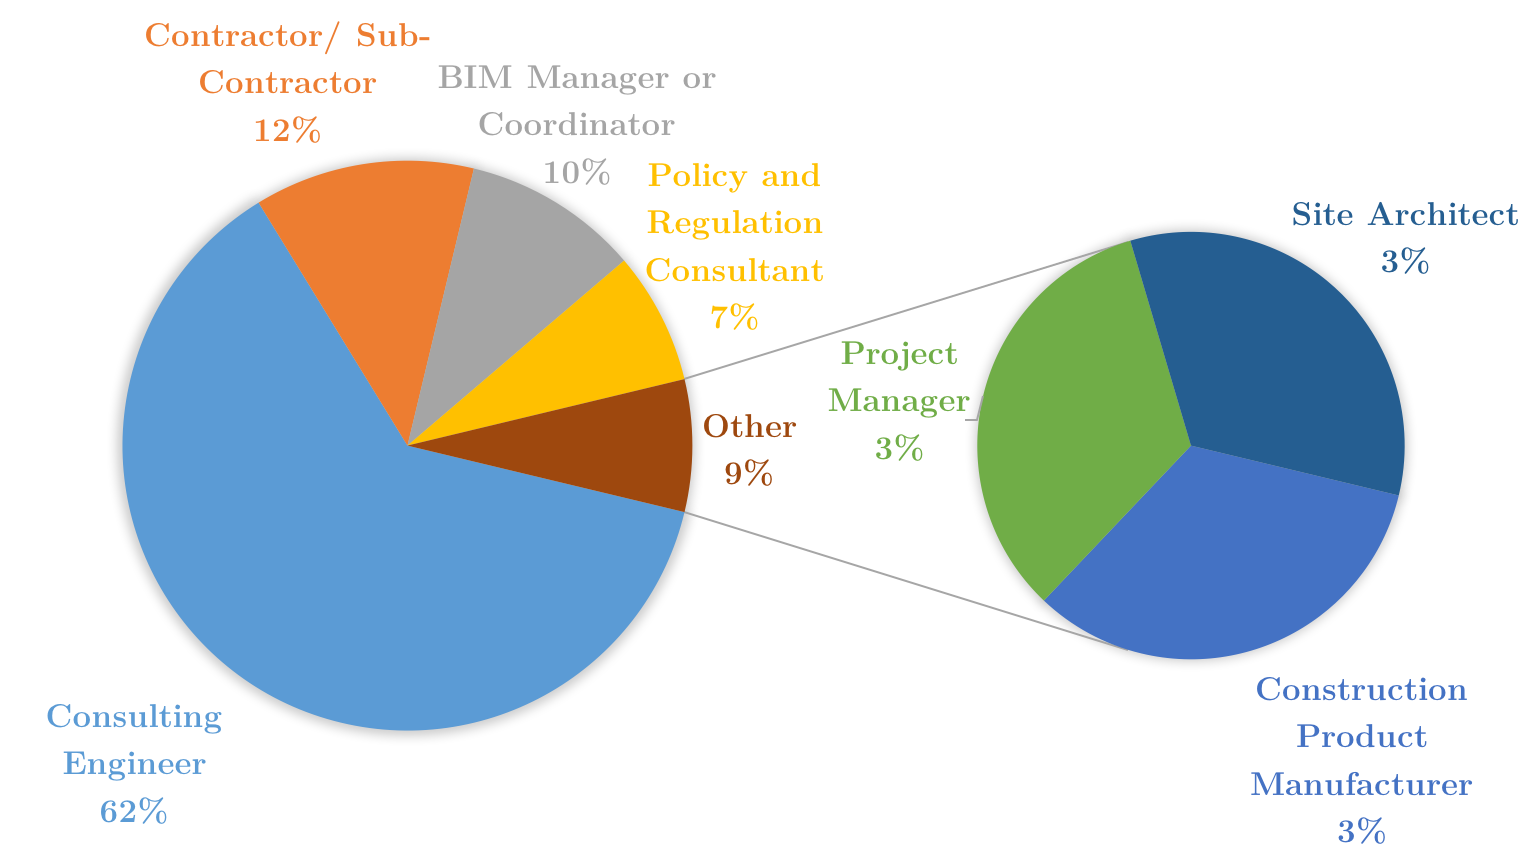
\includegraphics[width=\textwidth]{figures/positions.png}
	\rule{\textwidth}{0.5pt} % use line???
	\caption{Occupations of the survey respondents.}
	\label{positions}
\end{figure}


% Count has been used instead of percentage in certain graphs due to skewed responses…

90\% of the respondents work or have worked in building services, 79\% of whom were involved in one or more of the MEP fields (see Figure \ref{bs_fields}).
The respondents ranged in their number of years of experience in building services, from 0-5 years to more than 35 years (see Figure \ref{bs_yrs}).
Some of the respondents that have not directly worked in building services sometimes oversee or coordinate work by building services engineers.

% EXPANDED PIE CHART
\begin{figure}[htbp]
	\centering
	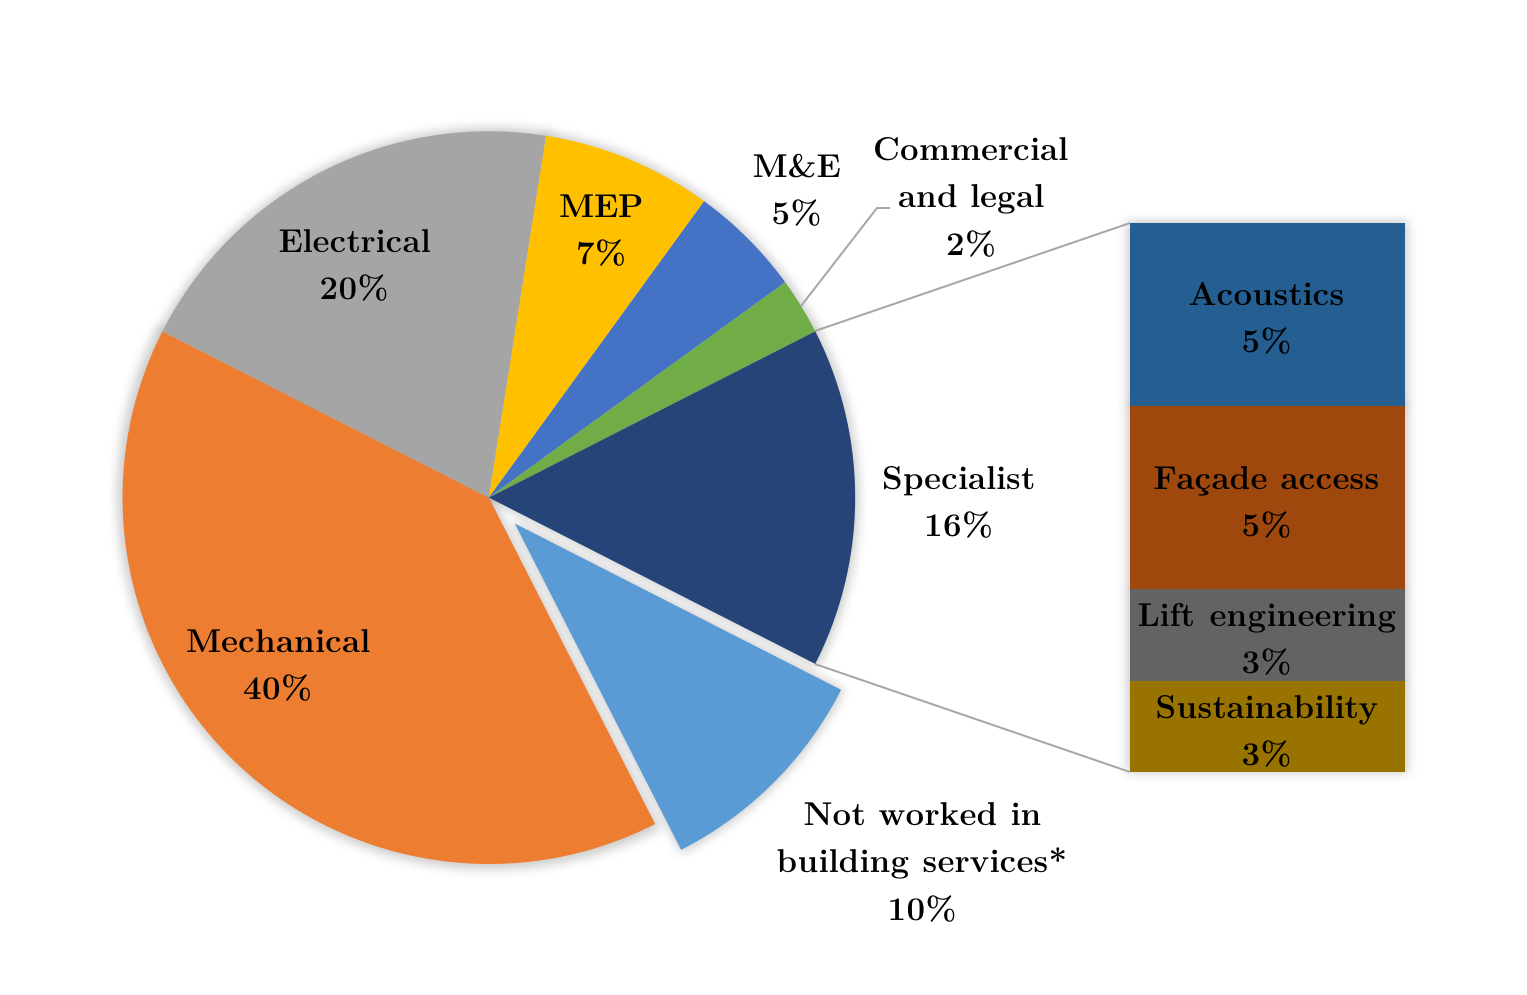
\includegraphics[width=\textwidth]{figures/BS-fields.png}
	\rule{\textwidth}{0.5pt} % use line???
	\caption[Building services fields of respondents.]{Building services fields of respondents. (*Some of these respondents either oversee work by building services engineers or coordinate between architectural, structural and MEP work.)}
	\label{bs_fields}
\end{figure}



% BAR CHART
\begin{figure}[htbp]
	\centering
	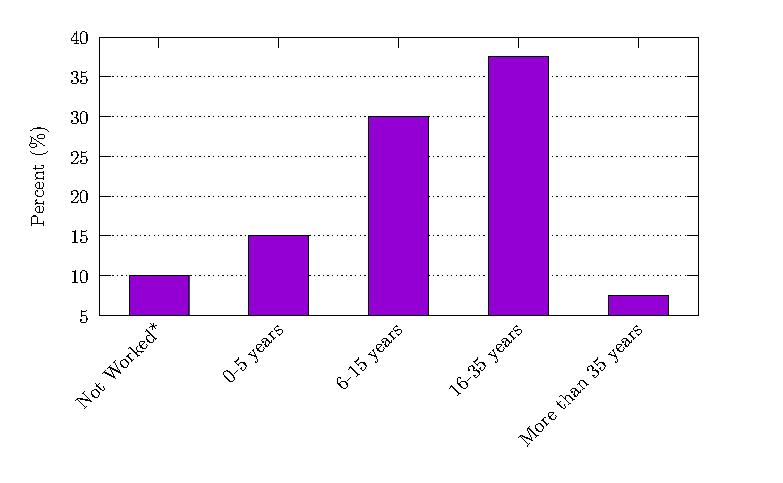
\includegraphics[width=\textwidth]{figures/Yrs-in-BS.eps}
	\rule{\textwidth}{0.5pt} % use line???
	\caption[Respondents' years working in building services.]{Respondents' years working in building services. (*These respondents have not worked in building services, but some of them either oversee work by building services engineers or coordinate between architectural, structural and MEP work.)}
	\label{bs_yrs}
\end{figure}

The respondents ranged in the number of years they had worked with BIM, from no experience to at least eight years' experience (see Figure \ref{bim_yrs}).
They also ranged in their confidence in working with BIM, with 43.6\% of the respondents considering themselves BIM literate, 38.5\% BIM illiterate, and 18\% neither nor (see Figure \ref{bim_literacy}).
% SPSS has been updated with currently 40 entries
It should be noted that the questionnaire did not define what was meant by `BIM literacy'.
Since BIM is an innovation in both technology and process, the respondents may have interpreted `BIM literacy' as their familiarity with either the technology, the process, or both.
Hence, the BIM literacy responses may be ambiguous.

As seen in Figure \ref{bim_literacy_X_bim_yrs}, there appears to be a correlation between the respondents' years of working with BIM and their BIM literacy.
100\% of the respondents that have worked with BIM for at least eight years and about 70\% of those that have worked with BIM for 3-7 years considered themselves BIM literate.
The responses of those with less or no experience in BIM peak at `Disagree'.
Interestingly, 30\% of those with less than two years' BIM experience and 12\% of those with no BIM experience considered themselves BIM literate.
% Perhaps they find themselves literate in BIM processes, as opposed to the technology.
% N.B. The questionnaire wasn't clear on what BIM literacy means and did not distinguish the BIM technology from the BIM process.

% BAR CHART
\begin{figure}[htbp]
	\centering
	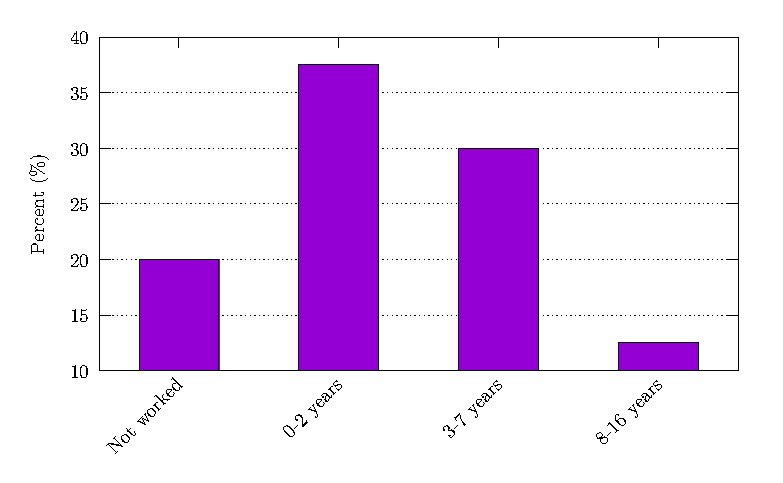
\includegraphics[width=\textwidth]{figures/BIM_yrs.eps}
	\rule{\textwidth}{0.5pt} % use line???
	\caption{Respondents' years working with BIM.}
	\label{bim_yrs}
\end{figure}


% BAR CHART
\begin{figure}[htbp]
	\centering
	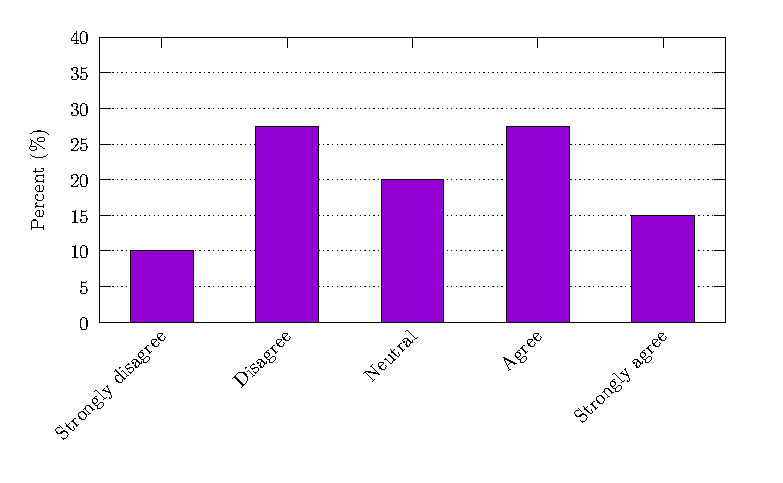
\includegraphics[width=\textwidth]{figures/BIM-literacy.eps}
	\rule{\textwidth}{0.5pt} % use line???
	\caption[Respondents' BIM literacy.]{Responses to the question ``How much do you agree with the statement `I am BIM literate'?".}
	\label{bim_literacy}
\end{figure}




% BAR CHART
\begin{figure}[htbp]
	\centering
	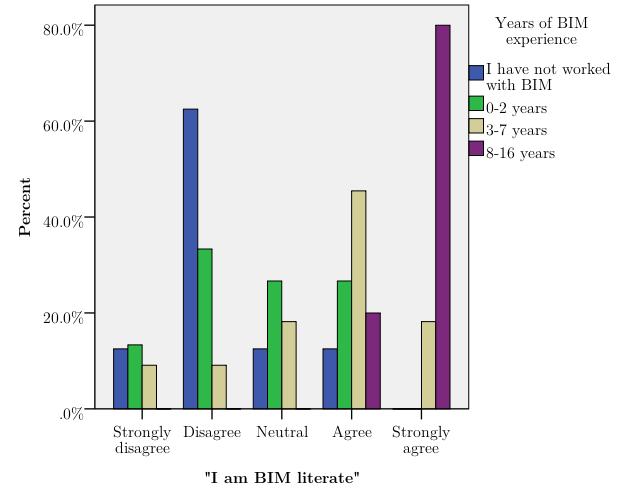
\includegraphics[width=0.9\textwidth]{figures/BIM_literacy_X_BIM_yrs.png}
	\rule{0.9\textwidth}{0.5pt} % use line???
	\caption{Respondents' years of BIM experience in terms of their BIM literacy.}
	\label{bim_literacy_X_bim_yrs}
\end{figure}

According to Figure \ref{bim_training_X_bim_literacy},
% compares the respondents' BIM literacy with their training in BIM.
there also appears to be a correlation between the respondents' BIM training and their BIM literacy.
Those with no or limited BIM experience are less confident in BIM.
BIM literacy ranges from illiterate to literate among the self-taught and those who received BIM training at the workplace.
Furthermore, it seems that people who are formally trained in BIM at university or college have greater confidence in their BIM abilities, but their sample size in this survey is too small to be sure.
% However, the sample size of people received BIM training at university or college was 
% There was also a range of BIM literacy responses depending on where respondents learned BIM.
% i.e. there is no correlation between BIM literacy and place of BIM training as far as we can tell.

% BAR CHART
\begin{figure}[htbp]
	\centering
	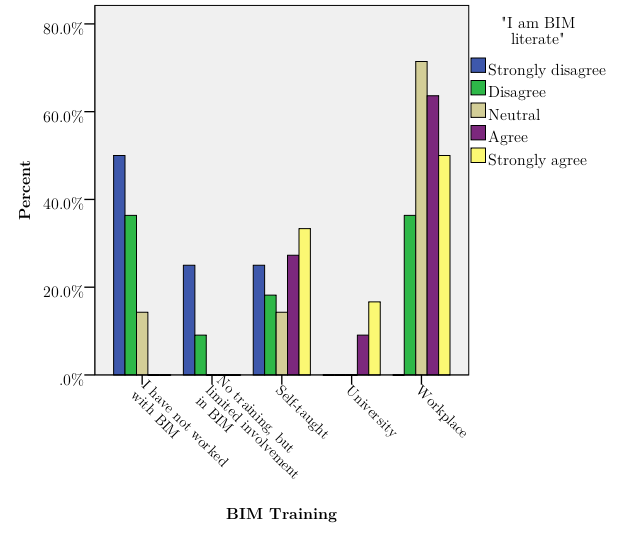
\includegraphics[width=0.9\textwidth]{figures/BIM_trainingXliteracy.png}
	\rule{0.9\textwidth}{0.5pt} % use line???
	\caption{Respondents' BIM literacy in terms of their BIM training.}
	\label{bim_training_X_bim_literacy}
\end{figure}

Figure \ref{position_X_bim_literacy} displays the respondents' BIM literacy in terms of their occupation.
As expected, 100\% of the BIM managers and coordinators considered themselves BIM literate.
Interestingly, there appears to be a wide range of BIM literacy among consulting engineers.
Figure \ref{consulting_X_bim_literacy} looks more closely at the consulting engineers' BIM literacy.
% Looking more closely at consulting engineers (them being our majority and focal point), 
None of the consulting engineers strongly agreed to being BIM literate.
Only 28\% considered themselves BIM literate, and almost 50\% considered themselves illiterate.


% BAR CHART
\begin{figure}[htbp]
	\centering
	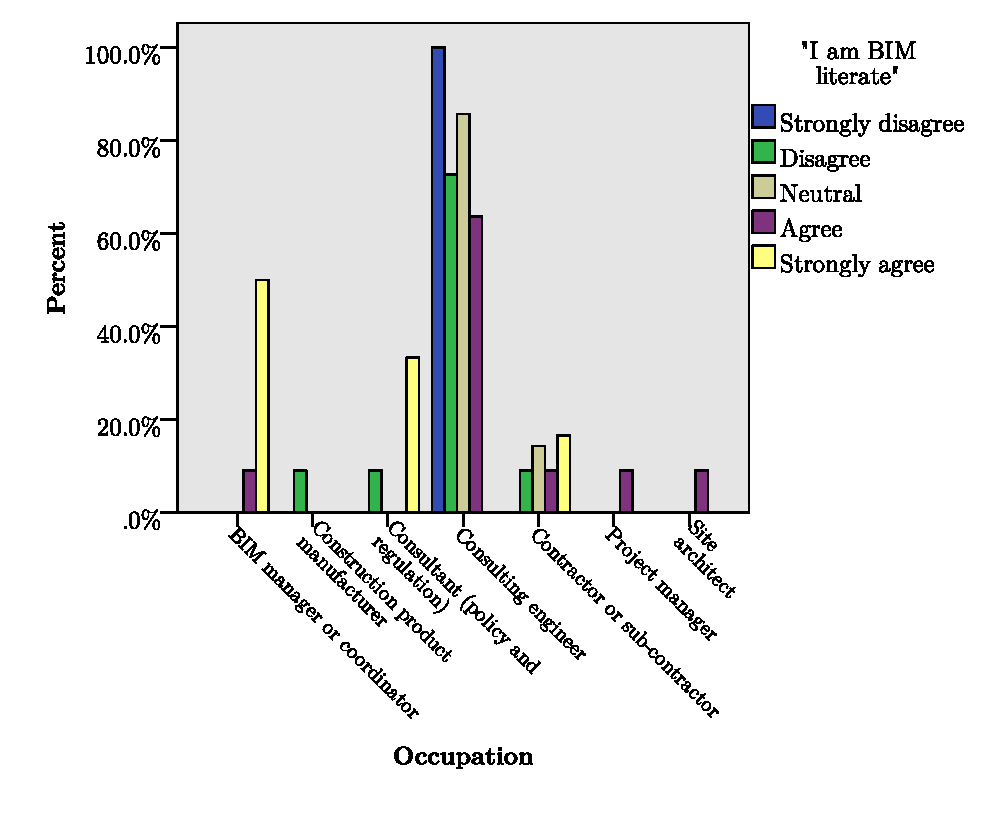
\includegraphics[width=0.9\textwidth]{figures/BIMLiteracyXPositions.eps}
	\rule{0.9\textwidth}{0.5pt} % use line???
	\caption{Respondents' BIM literacy in terms of their occupation.}
	\label{position_X_bim_literacy}
\end{figure}


% BAR CHART
\begin{figure}[htbp]
	\centering
	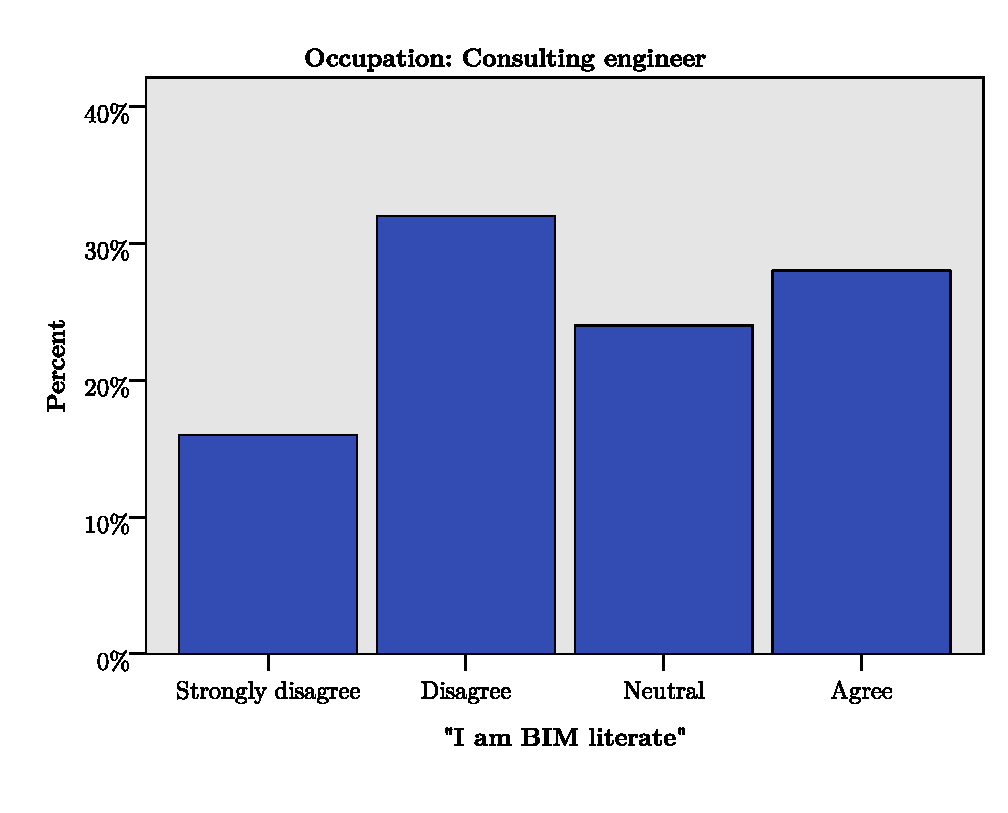
\includegraphics[width=0.9\textwidth]{figures/consultingXbimliteracy1.eps}
	\rule{0.9\textwidth}{0.5pt} % use line???
	\caption{Consulting engineers' BIM literacy.}
	\label{consulting_X_bim_literacy}
\end{figure}


%------------------------------
%	SUBSECTION 2
%------------------------------

\subsection{Contractors Only}

Only five of the respondents were contractors or sub-contractors.
All of these contractors have worked in building services for at least 16 years in either mechanical, or electrical, or both fields.
One of these contractors never receives Stage 4 BIM models from consultants, and another said that they were \say{not involved to that extent}.

Out of the remaining three contractors, two said that they typically receive generic and not necessarily coordinated Stage 4 models from consultants, and one said that they typically receive specific and spatially coordinated models.
One of the contractors that receives generic models typically finds that the models' intelligence breaks down when they replace generic objects with specific objects.
The other two do not seem to encounter this problem.

All three contractors typically re-build the consultant's BIM model.
They do this in spite of whether the model is specific and spatially coordinated to begin with, and in spite of not encountering BIM model breakdowns.
% So, why then do they do this?
% Is it not an unnecessary surplus of time and effort?

Finally, of the three contractors, only two send models to workshops for automatic fabrication of parts.
However, one of these respondents specified that they do this activity at Stage 5, not 4.

\begin{comment}
The two contractors that typically receive generic models have agreed to participate in an interview.
It would be interesting to speak with both of them, considering that:
\begin{itemize}
    \item They both have different experiences with model intelligence breaking down
    \item They both re-build models
    \item They both send out models to workshops for automatic fabrication of parts
\end{itemize}
\end{comment}


%------------------------------
%	SUBSECTION 3
%------------------------------

\subsection{Work Stage Deliverables}

The respondents were asked about their understanding of expected work stage deliverables.
This was done to verify whether there might indeed be a need to clarify MEP consultants' work stage deliverables, as \cite{Quigley2017} indicated.
% Therefore, this may contradict with what \cite{Quigley2017} said about there being a need to clarify what consulting MEP engineers need to deliver at each work stage.
88\% of the consulting engineers agreed or strongly agreed that they generally understand the level of information they are expected to deliver at the end of every work stage (see Figure \ref{consulting_X_understanding}).
8\% disagreed and 4\% were neutral.
One of those who disagreed, an experienced building services consulting engineer, explained that, \say{There is a lot of nonsense talked about BIM and poor specification of what is expected by those writing the contracts.}
One of those who responded neutrally, a building services consulting engineer with 6-15 years experience, explained that they \say{have an idea, but not the detail}.
One of those who agreed, an experienced building services consulting engineer, noted that they have an interpretation of what they believe each stage should look like, but that they \say{doubt if clients, contractors, etc… would agree as [it] is not set in stone as of yet}.

% BAR CHART
\begin{figure}[htbp]
	\centering
	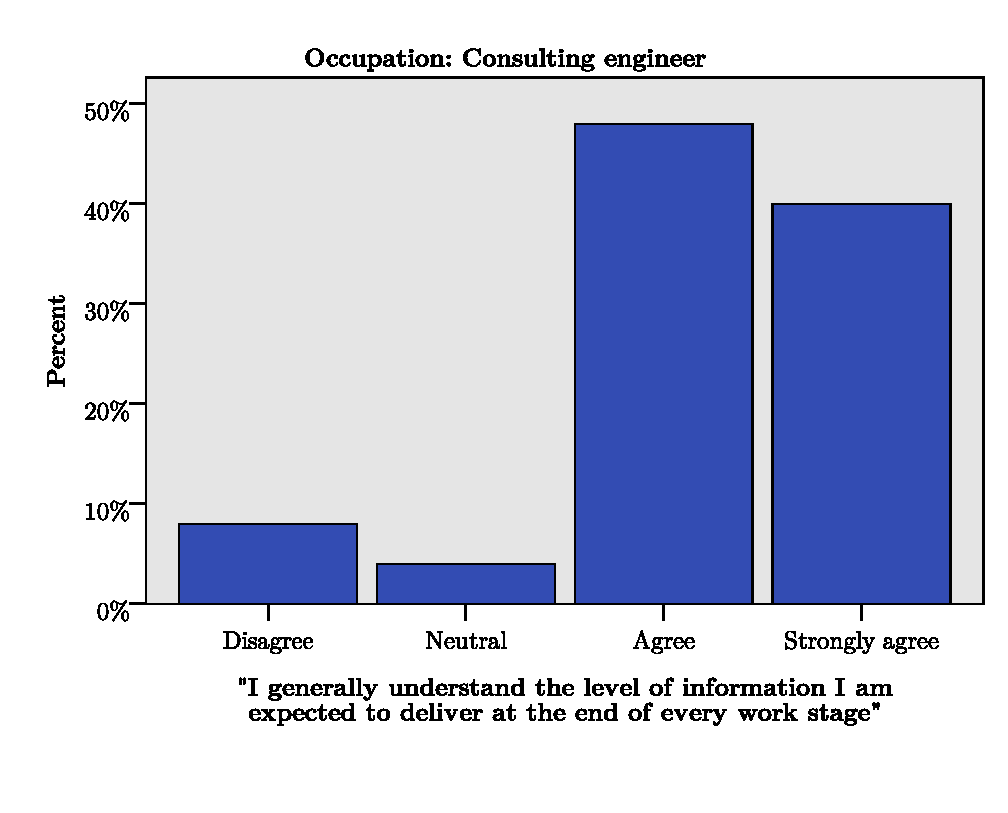
\includegraphics[width=0.9\textwidth]{figures/ConsultingXUnderstanding.eps}
	\rule{0.9\textwidth}{0.5pt} % use line???
	\caption{Consulting engineers' understanding of expected deliverables at the end of every work stage}
	\label{consulting_X_understanding}
\end{figure}


From an outside perspective, a project manager says the following: \say{I ordinarily am involved with setting the level that M\&E consultants are to deliver rather than delivering myself.  I generally find that M\&E consultants do understand what is required, but sometimes they resist delivering a high level of detail at early stages as they prefer to leave the detailed design to be done by sub-contractors}.
Our results (with 88\% consulting engineers agreeing to understand the work stage deliverables) reflect the project manager's observation of M\&E consultants generally understanding what is required.



%------------------------------
%	SUBSECTION 4
%------------------------------

\subsection{Levels of Definition}

The majority (60\%) of the respondents were familiar with the term LOD (see Figure \ref{LODfam}), whereas 17.5\% had never heard of the term.
The majority (56\%) of the consulting engineers, however, had either never heard of the term or were aware but not familiar with it.

% BAR CHART in count
\begin{figure}[htbp]
	\centering
	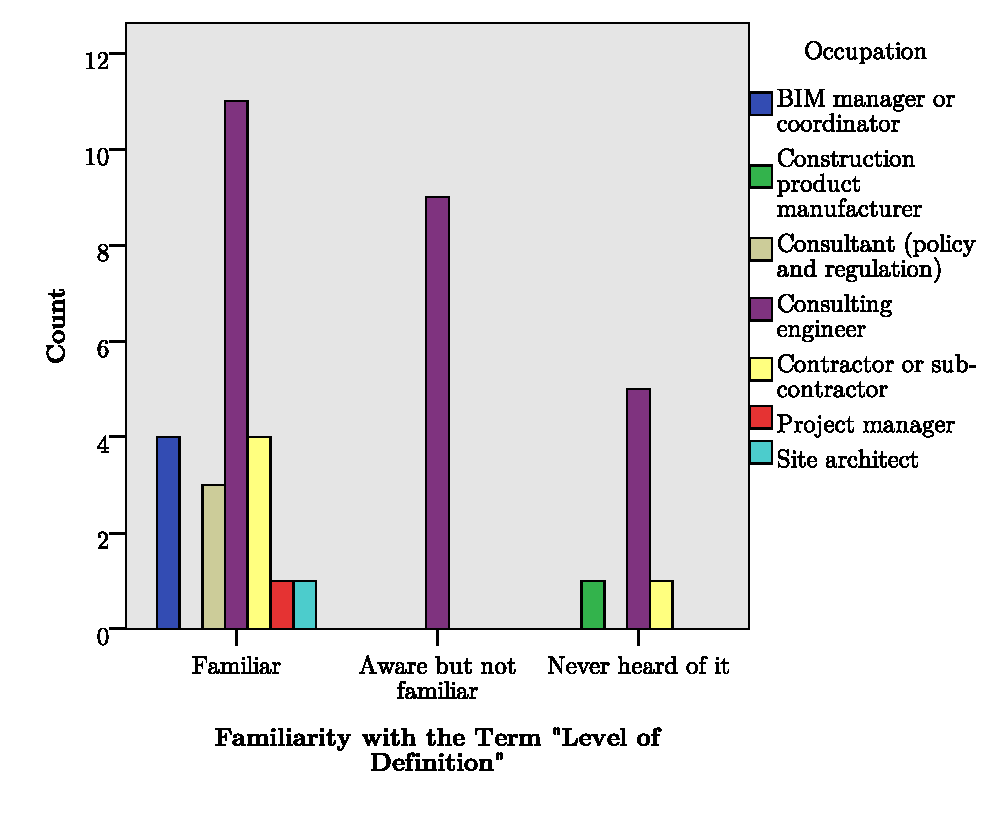
\includegraphics[width=0.9\textwidth]{figures/OccupationXLodCount.eps}
	\rule{0.9\textwidth}{0.5pt} % use line???
	\caption{Respondents' occupations in terms of their familiarity with the term LOD.}
	\label{LODfam}
\end{figure}


90\% and 92.5\% of the respondents accurately matched the term LoD with graphical content and the term LoI with non-graphical content, respectively (see Figure \ref{lod_loi}).
This can be seen as a positive outcome.
Despite 40\% of the respondents not being familiar with the term LOD, most of the respondents correctly matched the terms and definitions.
This may imply that LoD and LoI are fitting terms to indicate the amounts of graphical and non-graphical content in BIM models.
% It should be noted that the terms may \say{give themselves away} by their somewhat descriptiveness (for example, \say{level of \emph{information}} suits non-graphical content better than it does graphical), but that just goes to say that they are good names.

% BAR CHART in count???
\begin{figure}[htbp]
	\centering
	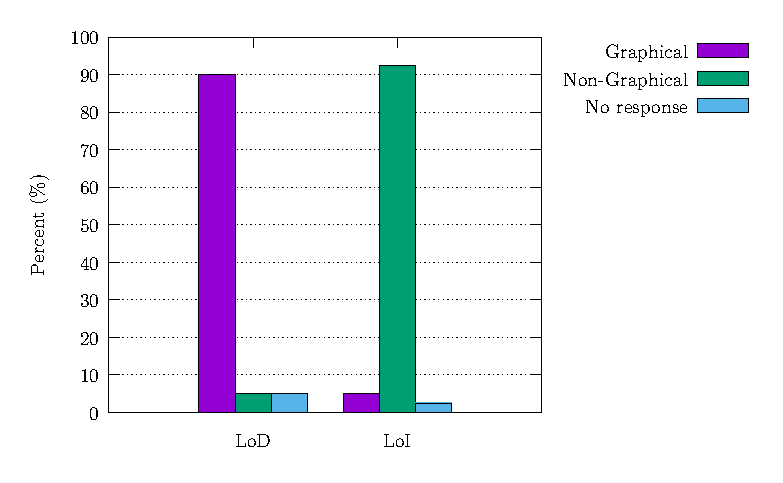
\includegraphics[width=0.9\textwidth]{figures/lod_loi.eps}
	\rule{0.9\textwidth}{0.5pt} % use line???
	\caption{Respondents' LoD and LoI term-and-definition matches.}
	\label{lod_loi}
\end{figure}


The open-ended question \say{Have you noticed a difference in levels of definition from one project to the next? If so, please describe,} received the most attention out of the five open-ended questions provided throughout the questionnaire, with responses from 52.5\% (21) of the respondents.

5\% (9.5\% of 21) of the respondents 
indicated that LODs did not apply to their work.
These respondents were specialist consulting building services engineers, working in either lift engineering/ vertical transportation or sustainability.

15\% (28.6\% of 21) of the respondents claimed to not have noticed any significant differences in LODs between projects.
Half of these respondents indicated that they follow standard LODs and directly mentioned one or more of the following sources that provide such:
the AIA,
the NBS BIM Toolkit,
PAS 1192-2,
and BSRIA's BG 6.
It may be interesting to note that these respondents consisted of a consulting building services engineer, a project manager, and a policy and regulation consultant.

However, 27.5\% (52.4\% of 21, the majority of this question's respondents) indicated that they do notice differences in LODs between projects.
These respondents consisted of consulting MEP and acoustics engineers, contractors/ sub-contractors, and policy and regulation consultants.
Some respondents
% \emph{enthusiastically/ strongly} 
stated that differences \say{definitely} or \say{regularly} occur between projects, and that these differences can be \say{large}.
The following points were gathered from similar comments from various respondents:
\begin{itemize}
    \item LODs are project-related, not work stage-related, and may depend on factors such as contractor and procurement route (e.g. design and build, or traditional).
    
    \item Clients producing Employer Information Requirements (EIRs) and others producing BIM Execution Plans (BEPs) do not fully understand what LODs mean, thus they do not understand what they are asking for in projects.
\end{itemize}

A consulting building services engineer illustrated the latter bullet point with an example of an educational building their team had recently designed.
The \say{BEP asked for LOD 400 throughout the project, even during early RIBA stages}.
The LOD referred to here is the AIA Level of Development 400.
According to \citeauthor{BIMForum2017} [\citeyear[p.~10]{BIMForum2017}], \say{An LOD 400 element is modeled at sufficient detail and accuracy for fabrication of the represented component. The quantity, size, shape, location, and orientation of the element as designed can be measured directly from the model without referring to non-modeled information such as notes or dimension call-outs.}
\cite{BIMForum2017} also indicates that LOD 400 represents the highest level of progression of model element geometry or non-graphic information.
Generally, it is unreasonable to expect such a high level of definition for building services during the early stages of a project.
Therefore, the client's lack of understanding of levels of definition can be seen in this example.

\begin{comment}
Interestingly, two policy and regulation consultants seem to \emph{disagree} on this question.
The first, with a background in architecture, construction project management and BIM, has not seen any differences in levels of definition between projects because they \say{generally use NBS for consistency}.
The other, with a background in building services, claims that \say{there is no actual definition of what the various LoDs mean, the interpretation always varies, though there are similar themes}.
This consultant's comment resonates with what is said in the \hl{BG6 (?)}…
\hl{why are different backgrounds significant?}
%\end{comment}xt

More interesting are the descriptive comments provided by BIM managers or coordinators.
One says, \say{The main problem is that projects don’t know what each LOD really means so [they] just ask for everything at 3 at stage 3, 4 at stage 4, etc. Or more likely 300, 350, as we mostly use the AIA definitions. 
Also architectural elements are often more progressed at each stage than MEP, which causes confusion. 
LOD is often mistaken for meaning coordination but really they don’t describe coordination at all, just detail!}
% \hl{What kind of coordination: rates of progression of different design aspects, or coordination of A, MEP and S models?}
We learn three things here:
\begin{enumerate}
    \item Clients can easily perceive LODs to be work stage-related, rather than project-related, and define LODs as blanket values for the whole project, changing at each stage.
    This may be due to the seemingly correlated numbering systems of the RIBA PoW 2013 and the LODs. % \hl{what about AIA levels?}
    
    \item The fact that different aspects of a design (e.g. architecture, building services and structure) may progress at different rates is a concept that appears to confuse clients.
    
    \item Perhaps due to the assumption that LODs are work stage-related and apply to all disciplines, LODs are often mistaken for referring to the coordination of the rates of progression of different design aspects.
    The use of the phrase \say{levels of coordination/detail} in a response by a consulting building services engineer partially confirms the presence of this confusion.
\end{enumerate}

Another BIM manager or coordinator laments about the \say{unnecessary, confusing, and impractical} nature of the current LODs.
They go on to say that their team or organisation have actually implemented an alternative approach.
The author attempted to follow up this respondent to find out more about the alternative approach they use and their reason for abandoning LODs, but the author was unable to reach the respondent.
% Because this respondent has agreed to a follow-up interview and seems to be experienced, knowledgeable and passionate about the topic of levels of definition, I would like to speak further with them.



%------------------------------
%	SUBSECTION 5
%------------------------------

\subsection{Match the Image with the Work Stage}

Respondents were asked to match RIBA PoW 2013 stages with a sample of pictures of various LODs as defined by the NBS BIM Toolkit and % various work stage progressions as defined by 
the BG 6 (see Figures \ref{image1} to \ref{image6}).
% Pictures of LODs 3-5 were used.
% , our main interest being in Stage/ LOD 4; 3 and 5 were used for \say{control} purposes.
It should be noted that LoDs 4 and 5 can easily be confused.
For instance, the only difference between the two LoDs may be the presence of fixing systems in LOD 5.
Therefore, the author did not consider respondents who answered LoD 4 to be incorrect when the actual LoD was 5, and vice-versa.

This activity showed that there was a general agreement among the respondents about the amount of graphical content that the NBS and BSRIA expect at various work stages.
The majority of the respondents correctly matched all of the LODs with the work stages, except for in the third image (see Figure \ref{image3}).
A possible reason for the majority getting this image wrong is that the image would be mostly familiar to electrical and fire engineers, which only 32\% of the respondents may have worked as (see Figure \ref{bs_fields}).
% Although only a third of the respondents were correct about the first image corresponding to Stage 5 (see Figure \ref{image1}), but it should be noted that LoD 5 can easily be confused with LoD 4.

% \hl{See what specifically consulting engineers voted?}


%%% 1
\begin{figure}[htbp]
\centering
  \begin{subfigure}[b]{.35\textwidth}
  \centering
  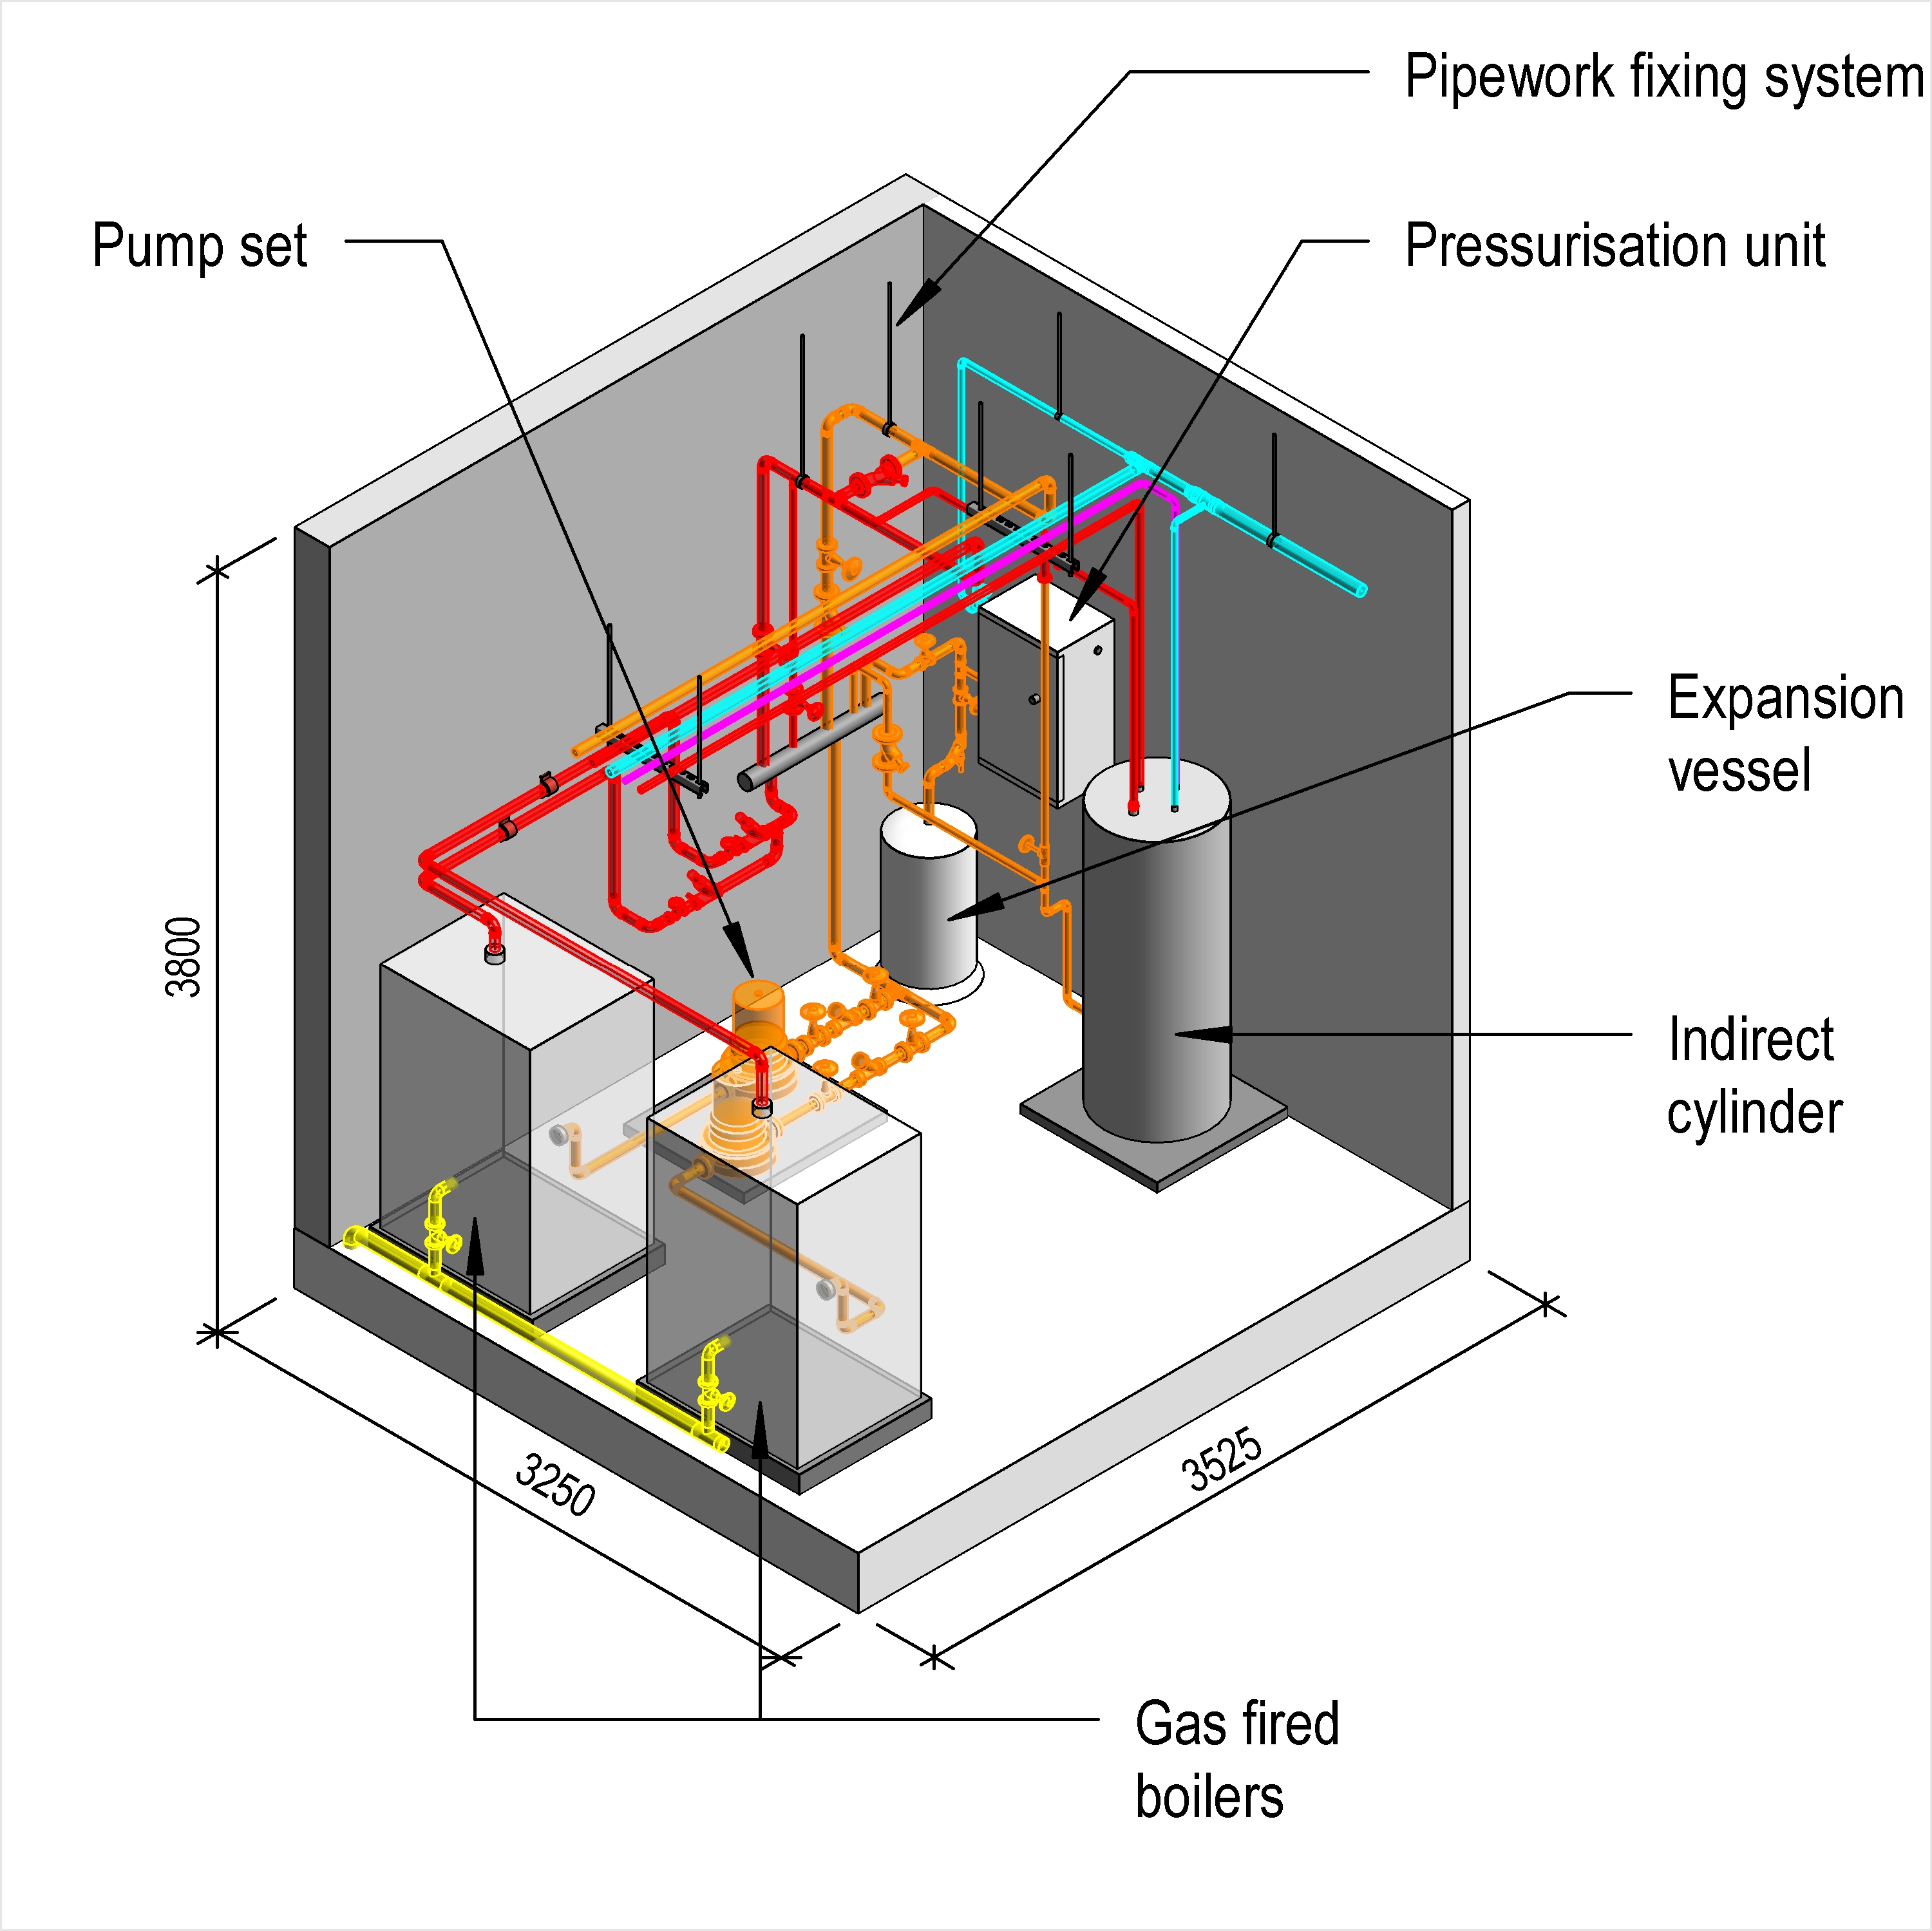
\includegraphics[width=\textwidth]{figures/MTHW-heating-systems.jpg}
		\rule{\textwidth}{0.5pt} % use line???
  \caption{NBS LoD 5}
  \label{}
\end{subfigure}
  \begin{subfigure}[b]{.61\textwidth}
  \centering
  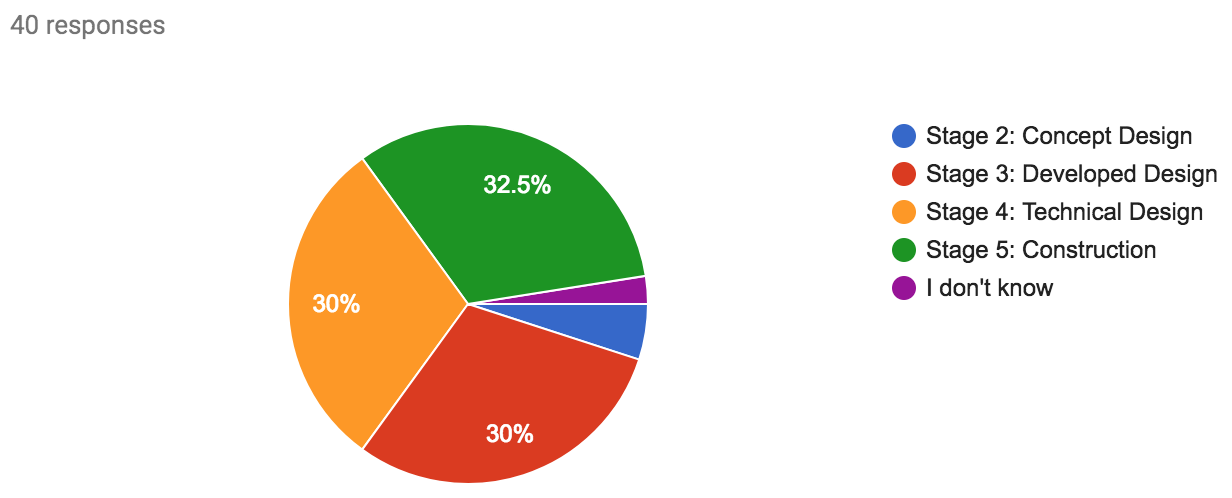
\includegraphics[width=\textwidth]{figures/image1.png}
 		\rule{\textwidth}{0.5pt} % use line???
  \caption{Responses}
  \label{}
\end{subfigure}
\caption[The actual and guessed LoDs of the first image in the ``Match the Image with the Work Stage" activity.]{({\scriptsize A}) The actual LoD and ({\scriptsize B}) the respondents’ guessed LoD of the first image in the ``Match the Image with the Work Stage" activity.}
\label{image1}
\end{figure}
%%%



%%% 2
\begin{figure}[htbp]
\centering
  \begin{subfigure}[b]{.35\textwidth}
  \centering
  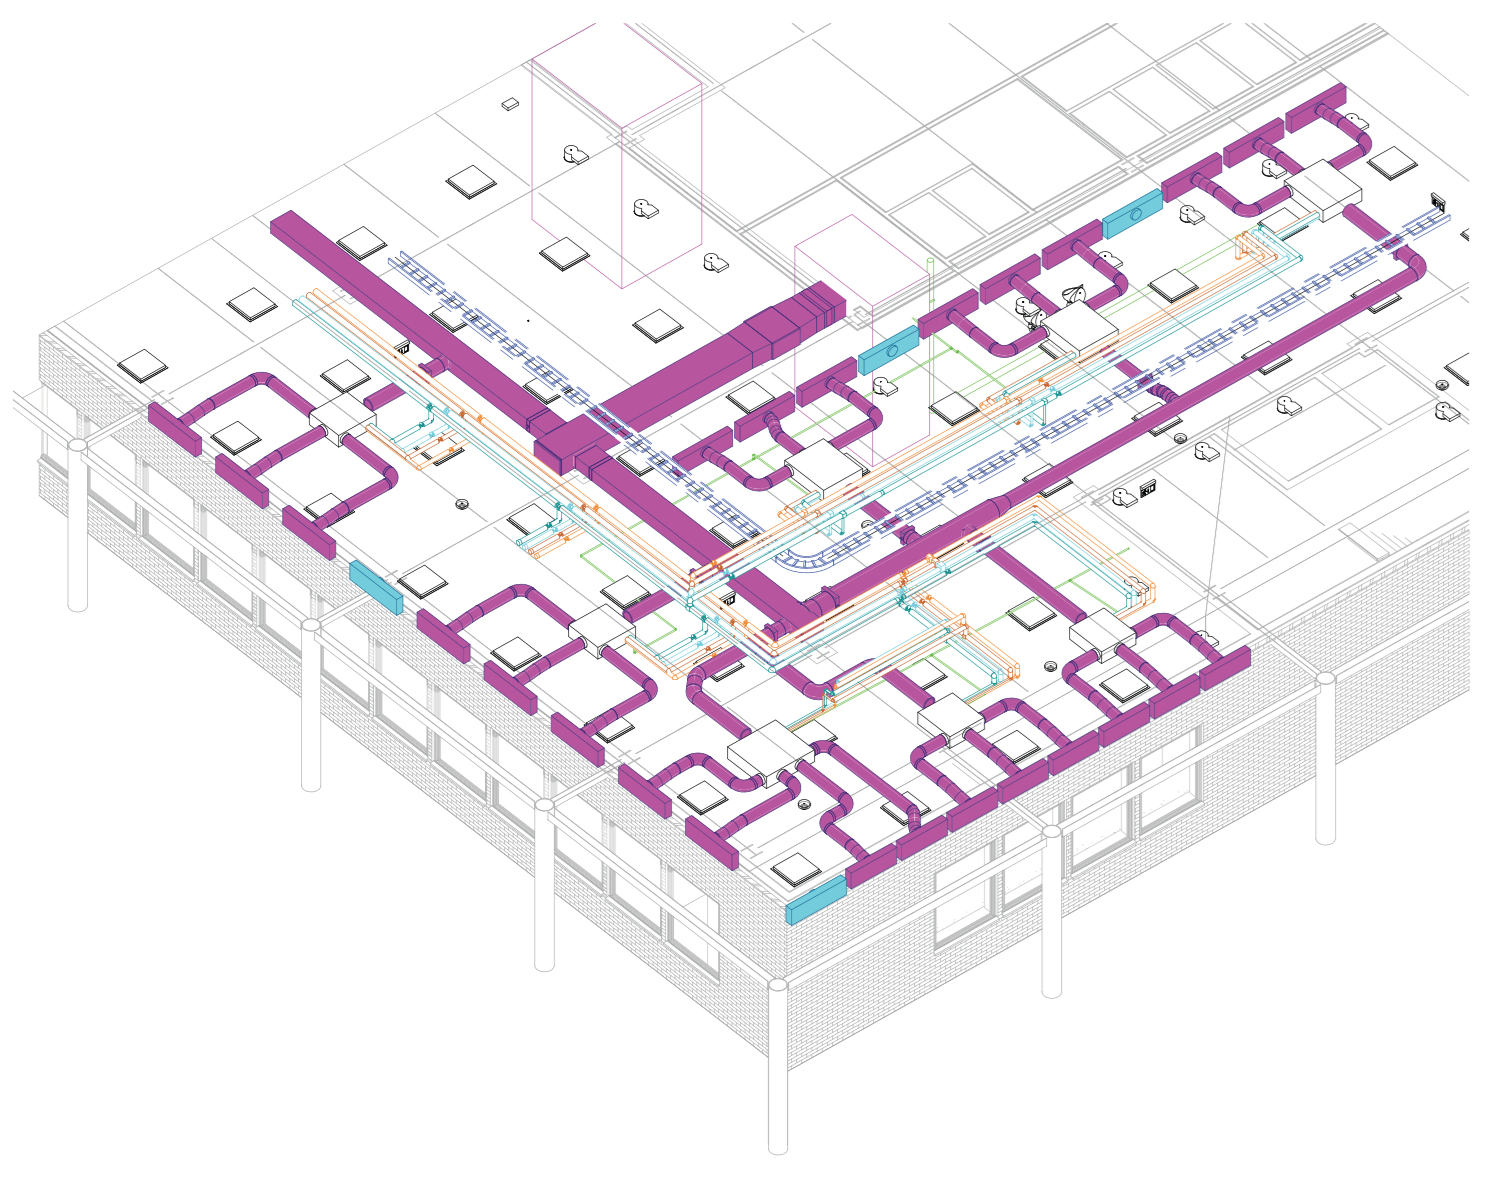
\includegraphics[width=\textwidth]{figures/4bModel01.png}
 		\rule{\textwidth}{0.5pt} % use line???
  \caption{BG6 Model Definition 4b}
  \label{}
\end{subfigure}
  \begin{subfigure}[b]{.61\textwidth}
  \centering
  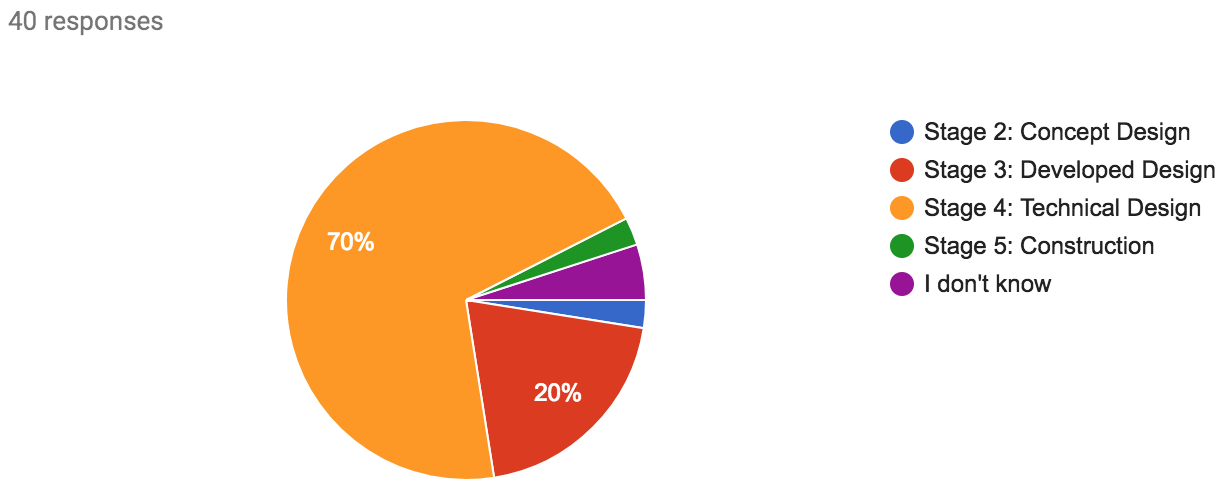
\includegraphics[width=\textwidth]{figures/image2.png}
		\rule{\textwidth}{0.5pt} % use line???
  \caption{Responses}
  \label{}
\end{subfigure}
\caption[The actual and guessed LoDs of the second image in the ``Match the Image with the Work Stage" activity.]{({\scriptsize A}) The actual LoD and ({\scriptsize B}) the respondents’ guessed LoD of the second image in the ``Match the Image with the Work Stage" activity.}
\label{image2}
\end{figure}
%%%



%%% 3
\begin{figure}[htbp]
\centering
  \begin{subfigure}[b]{.35\textwidth}
  \centering
  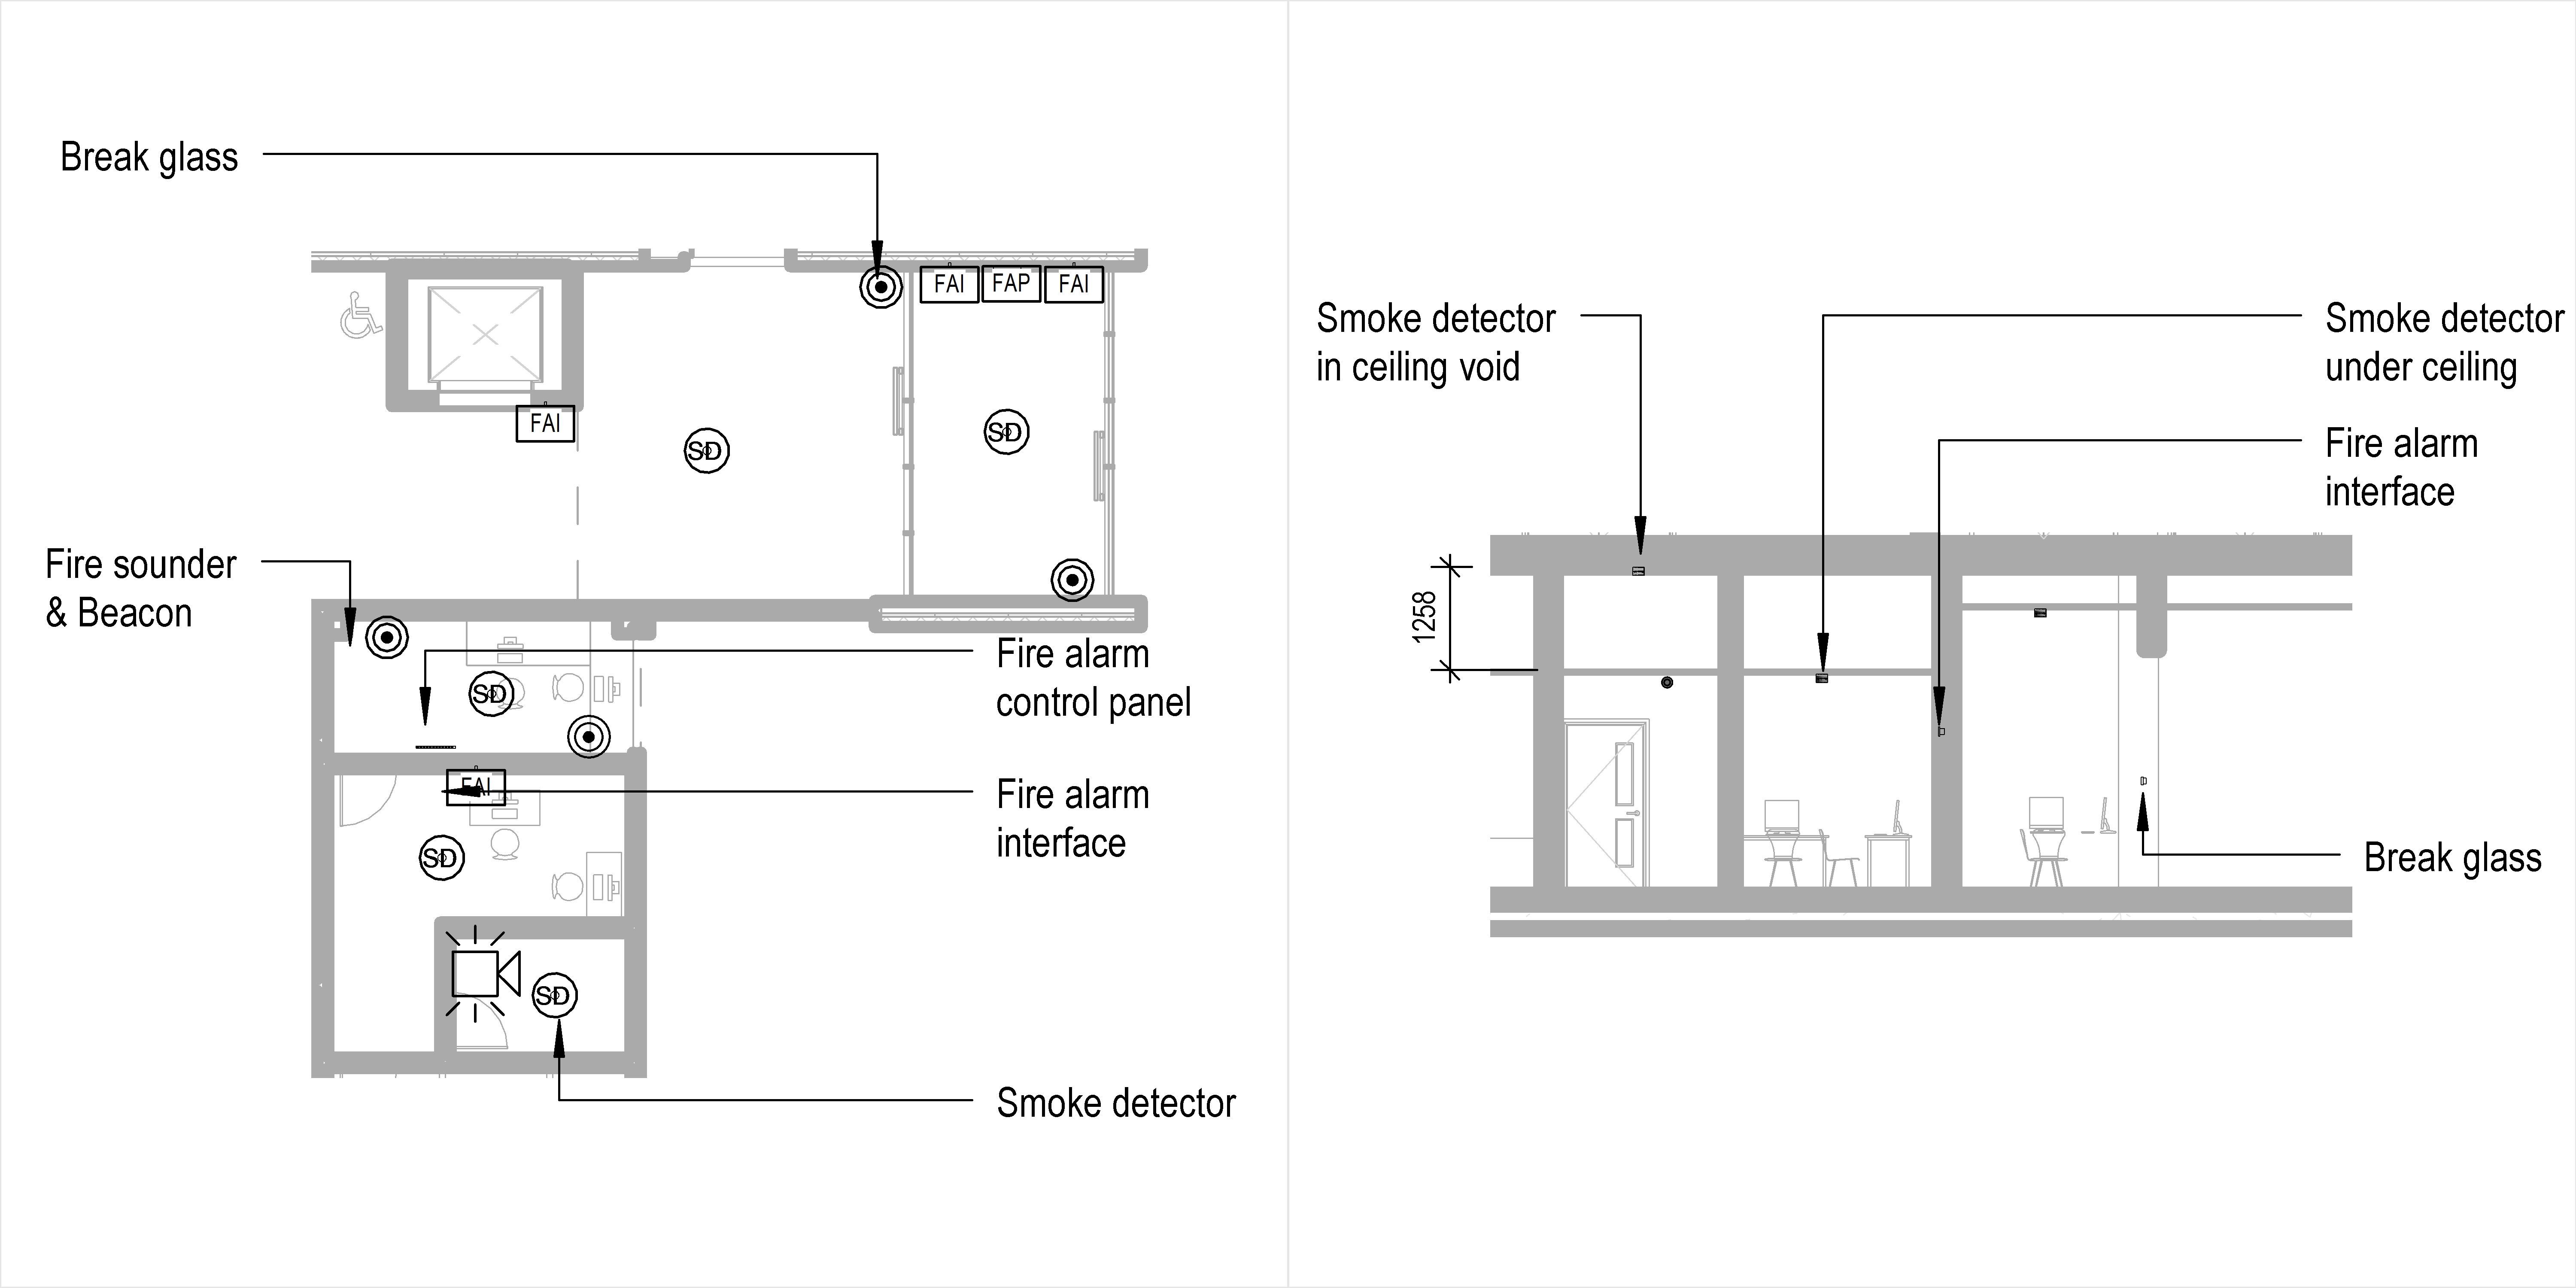
\includegraphics[width=\textwidth]{figures/fire-combined.png}
		\rule{\textwidth}{0.5pt} % use line???
  \caption{NBS LoD 4}
  \label{}
\end{subfigure}
  \begin{subfigure}[b]{.61\textwidth}
  \centering
  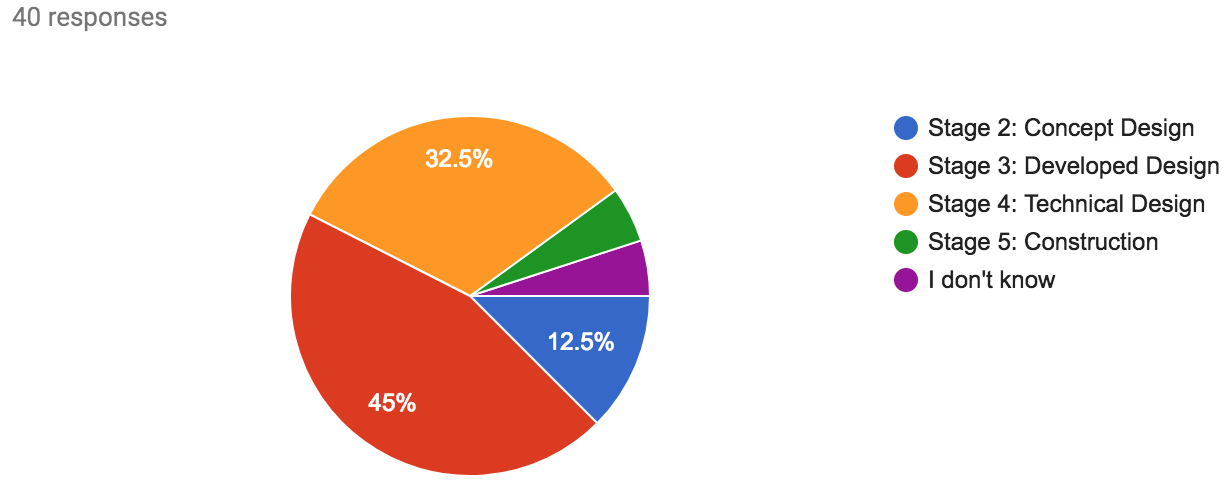
\includegraphics[width=\textwidth]{figures/image3.png}
		\rule{\textwidth}{0.5pt} % use line???
  \caption{Responses}
  \label{}
\end{subfigure}
\caption[The actual and guessed LoDs of the third image in the ``Match the Image with the Work Stage" activity.]{({\scriptsize A}) The actual LoD and ({\scriptsize B}) the respondents’ guessed LoD of the third image in the ``Match the Image with the Work Stage" activity.}
\label{image3}
\end{figure}
%%%



%%% 4
\begin{figure}[htbp]
\centering
  \begin{subfigure}[b]{.35\textwidth}
  \centering
  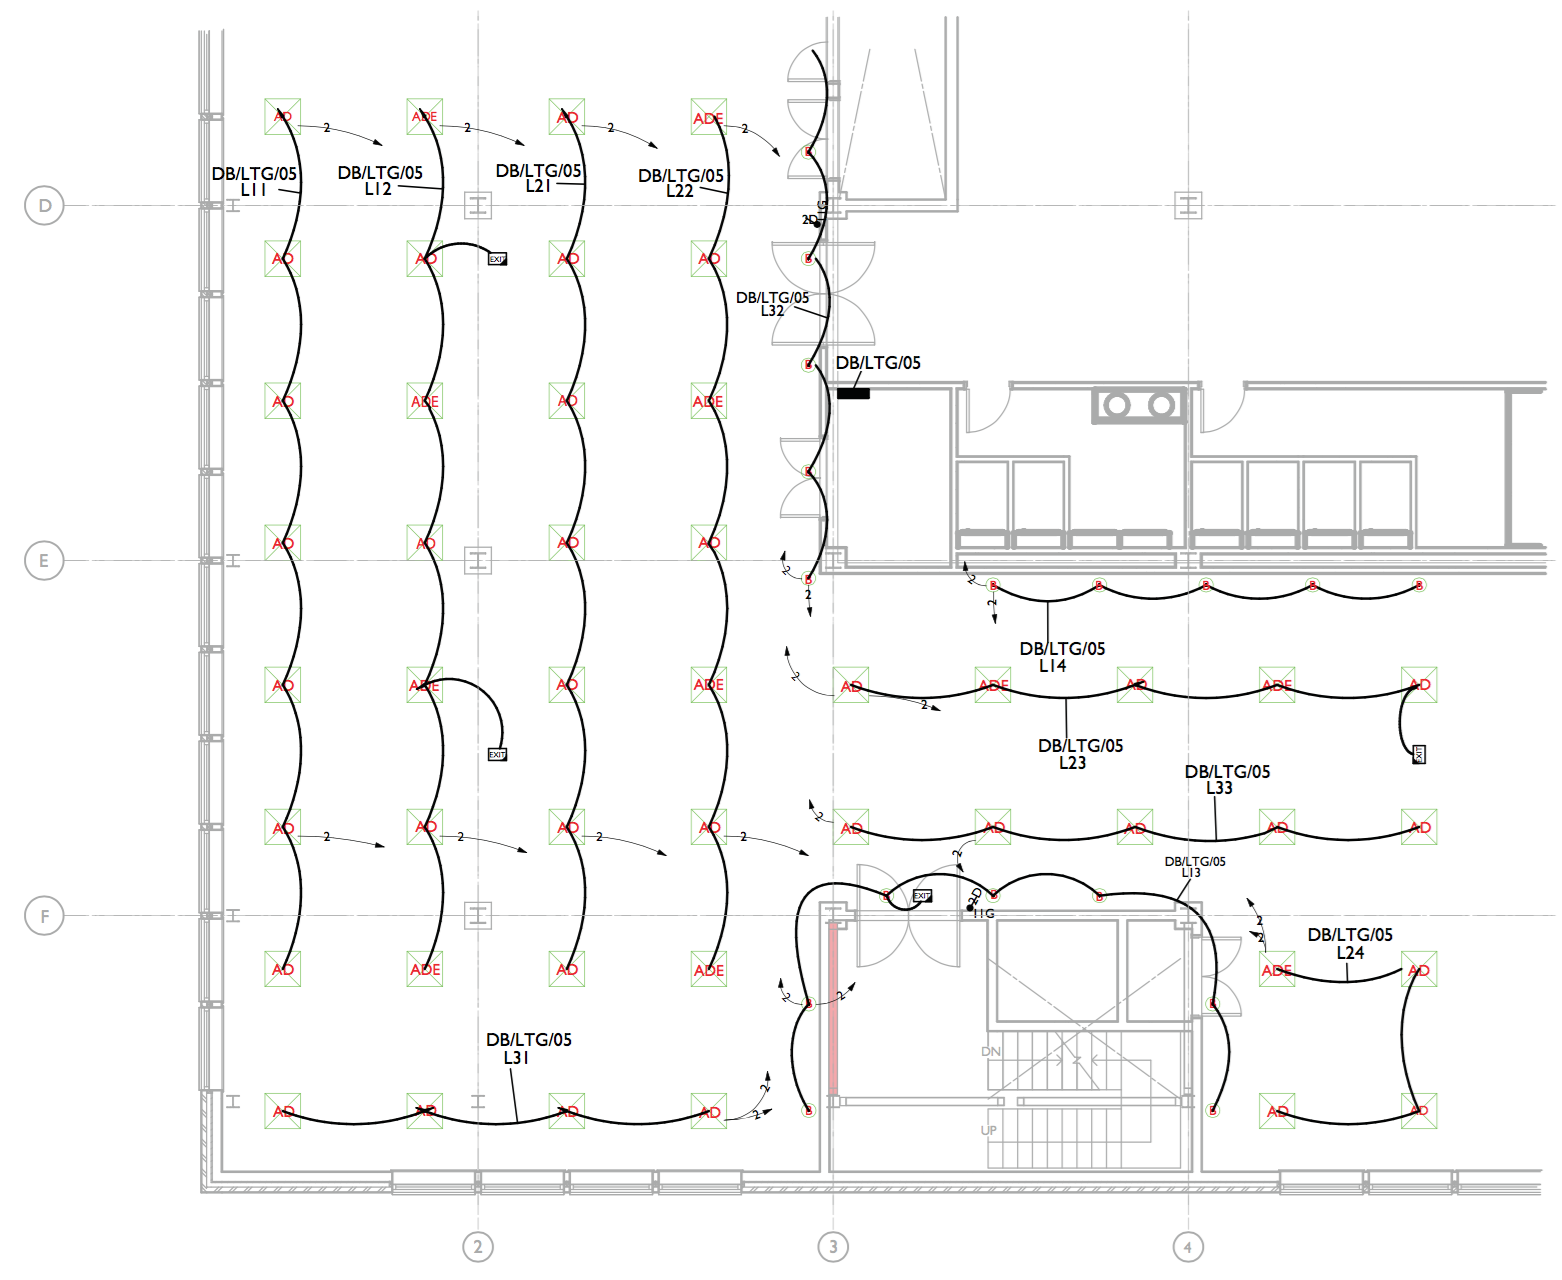
\includegraphics[width=\textwidth]{figures/4aDwg02.png}
		\rule{\textwidth}{0.5pt} % use line???
  \caption{BG6 Drawing Definition 4a}
  \label{}
\end{subfigure}
  \begin{subfigure}[b]{.61\textwidth}
  \centering
  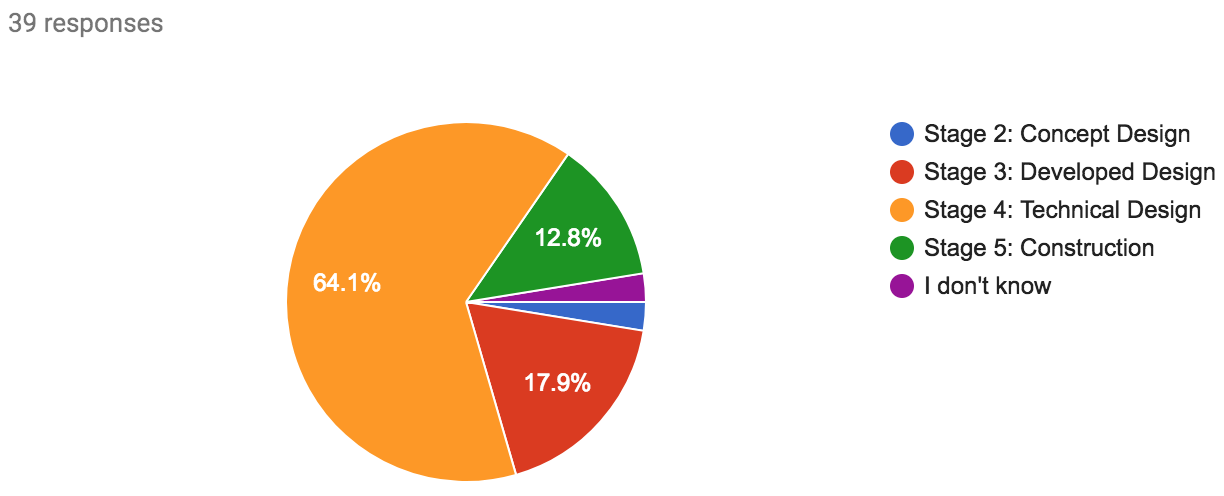
\includegraphics[width=\textwidth]{figures/image4.png}
		\rule{\textwidth}{0.5pt} % use line???
  \caption{Responses}
  \label{}
\end{subfigure}
\caption[The actual and guessed LoDs of the fourth image in the ``Match the Image with the Work Stage" activity.]{({\scriptsize A}) The actual LoD and ({\scriptsize B}) the respondents’ guessed LoD of the fourth image in the ``Match the Image with the Work Stage" activity.}
\label{image4}
\end{figure}
%%%



%%% 5
\begin{figure}[htbp]
\centering
  \begin{subfigure}[b]{.35\textwidth}
  \centering
  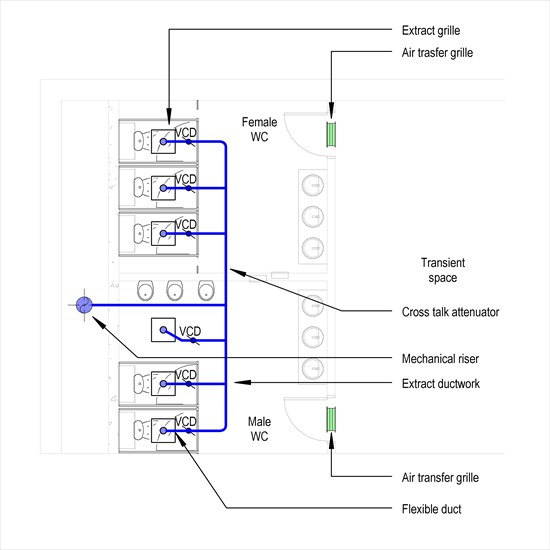
\includegraphics[width=\textwidth]{figures/local-exhaust-vent-syst.jpg}
		\rule{\textwidth}{0.5pt} % use line???
  \caption{NBS LoD 3}
  \label{}
\end{subfigure}
  \begin{subfigure}[b]{.61\textwidth}
  \centering
  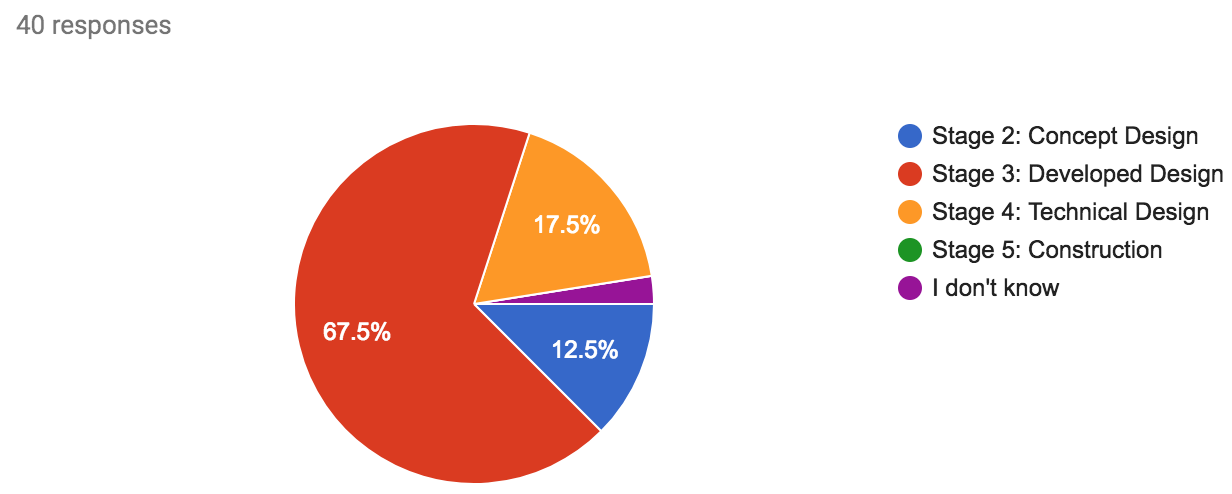
\includegraphics[width=\textwidth]{figures/image5.png}
		\rule{\textwidth}{0.5pt} % use line???
  \caption{Responses}
  \label{}
\end{subfigure}
\caption[The actual and guessed LoDs of the fifth image in the ``Match the Image with the Work Stage" activity.]{({\scriptsize A}) The actual LoD and ({\scriptsize B}) the respondents’ guessed LoD of the fifth image in the ``Match the Image with the Work Stage" activity.}
\label{image5}
\end{figure}
%%%



%%% 6
\begin{figure}[htbp]
\centering
  \begin{subfigure}[b]{.35\textwidth}
  \centering
  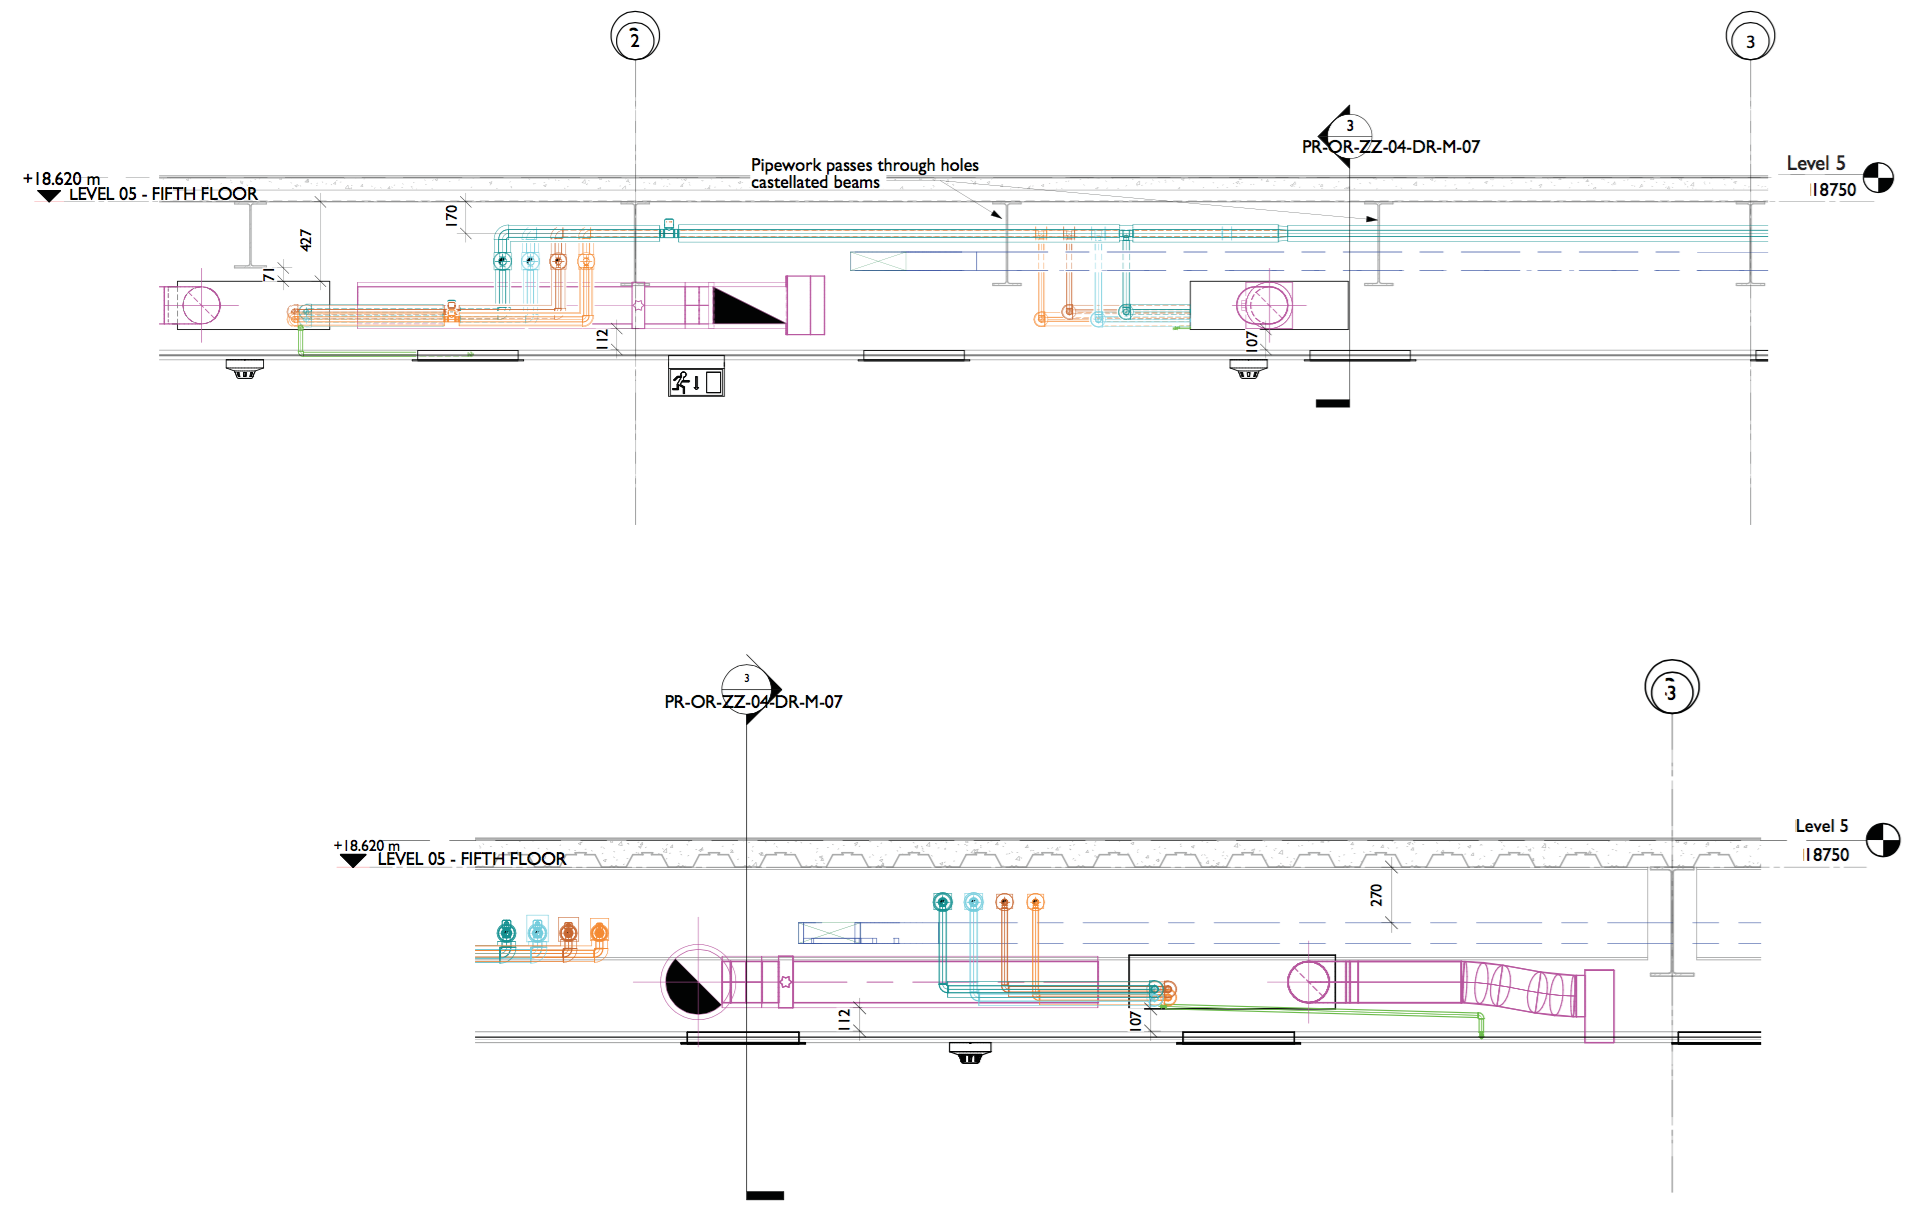
\includegraphics[width=\textwidth]{figures/4bCoordDwg02.png}
		\rule{\textwidth}{0.5pt} % use line???
  \caption{BG6 Drawing Definition 4b}
  \label{}
\end{subfigure}
  \begin{subfigure}[b]{.61\textwidth}
  \centering
  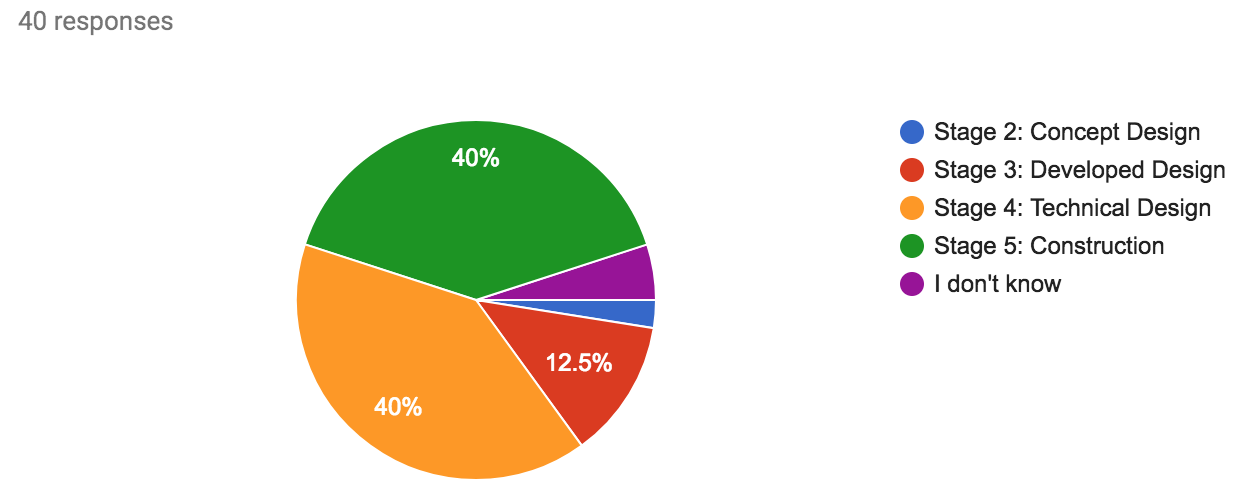
\includegraphics[width=\textwidth]{figures/image6.png}
		\rule{\textwidth}{0.5pt} % use line???
  \caption{Responses}
  \label{}
\end{subfigure}
\caption[The actual and guessed LoDs of the sixth image in the ``Match the Image with the Work Stage" activity.]{({\scriptsize A}) The actual LoD and ({\scriptsize B}) the respondents’ guessed LoD of the sixth image in the ``Match the Image with the Work Stage" activity.}
\label{image6}
\end{figure}
%%%




%------------------------------
%	SUBSECTION 6
%------------------------------

\newpage
\subsection{Documents}

This section of the questionnaire asked the respondents if they were familiar with PAS 1192-2, BG 6 and ACE Schedule of Services MEP (see Figures \ref{pas} to \ref{ace}).
The respondents were most familiar with the BG 6, and least familiar with the ACE Schedule of Services MEP.

% PIE CHART
\begin{figure}[htbp]
	\centering
	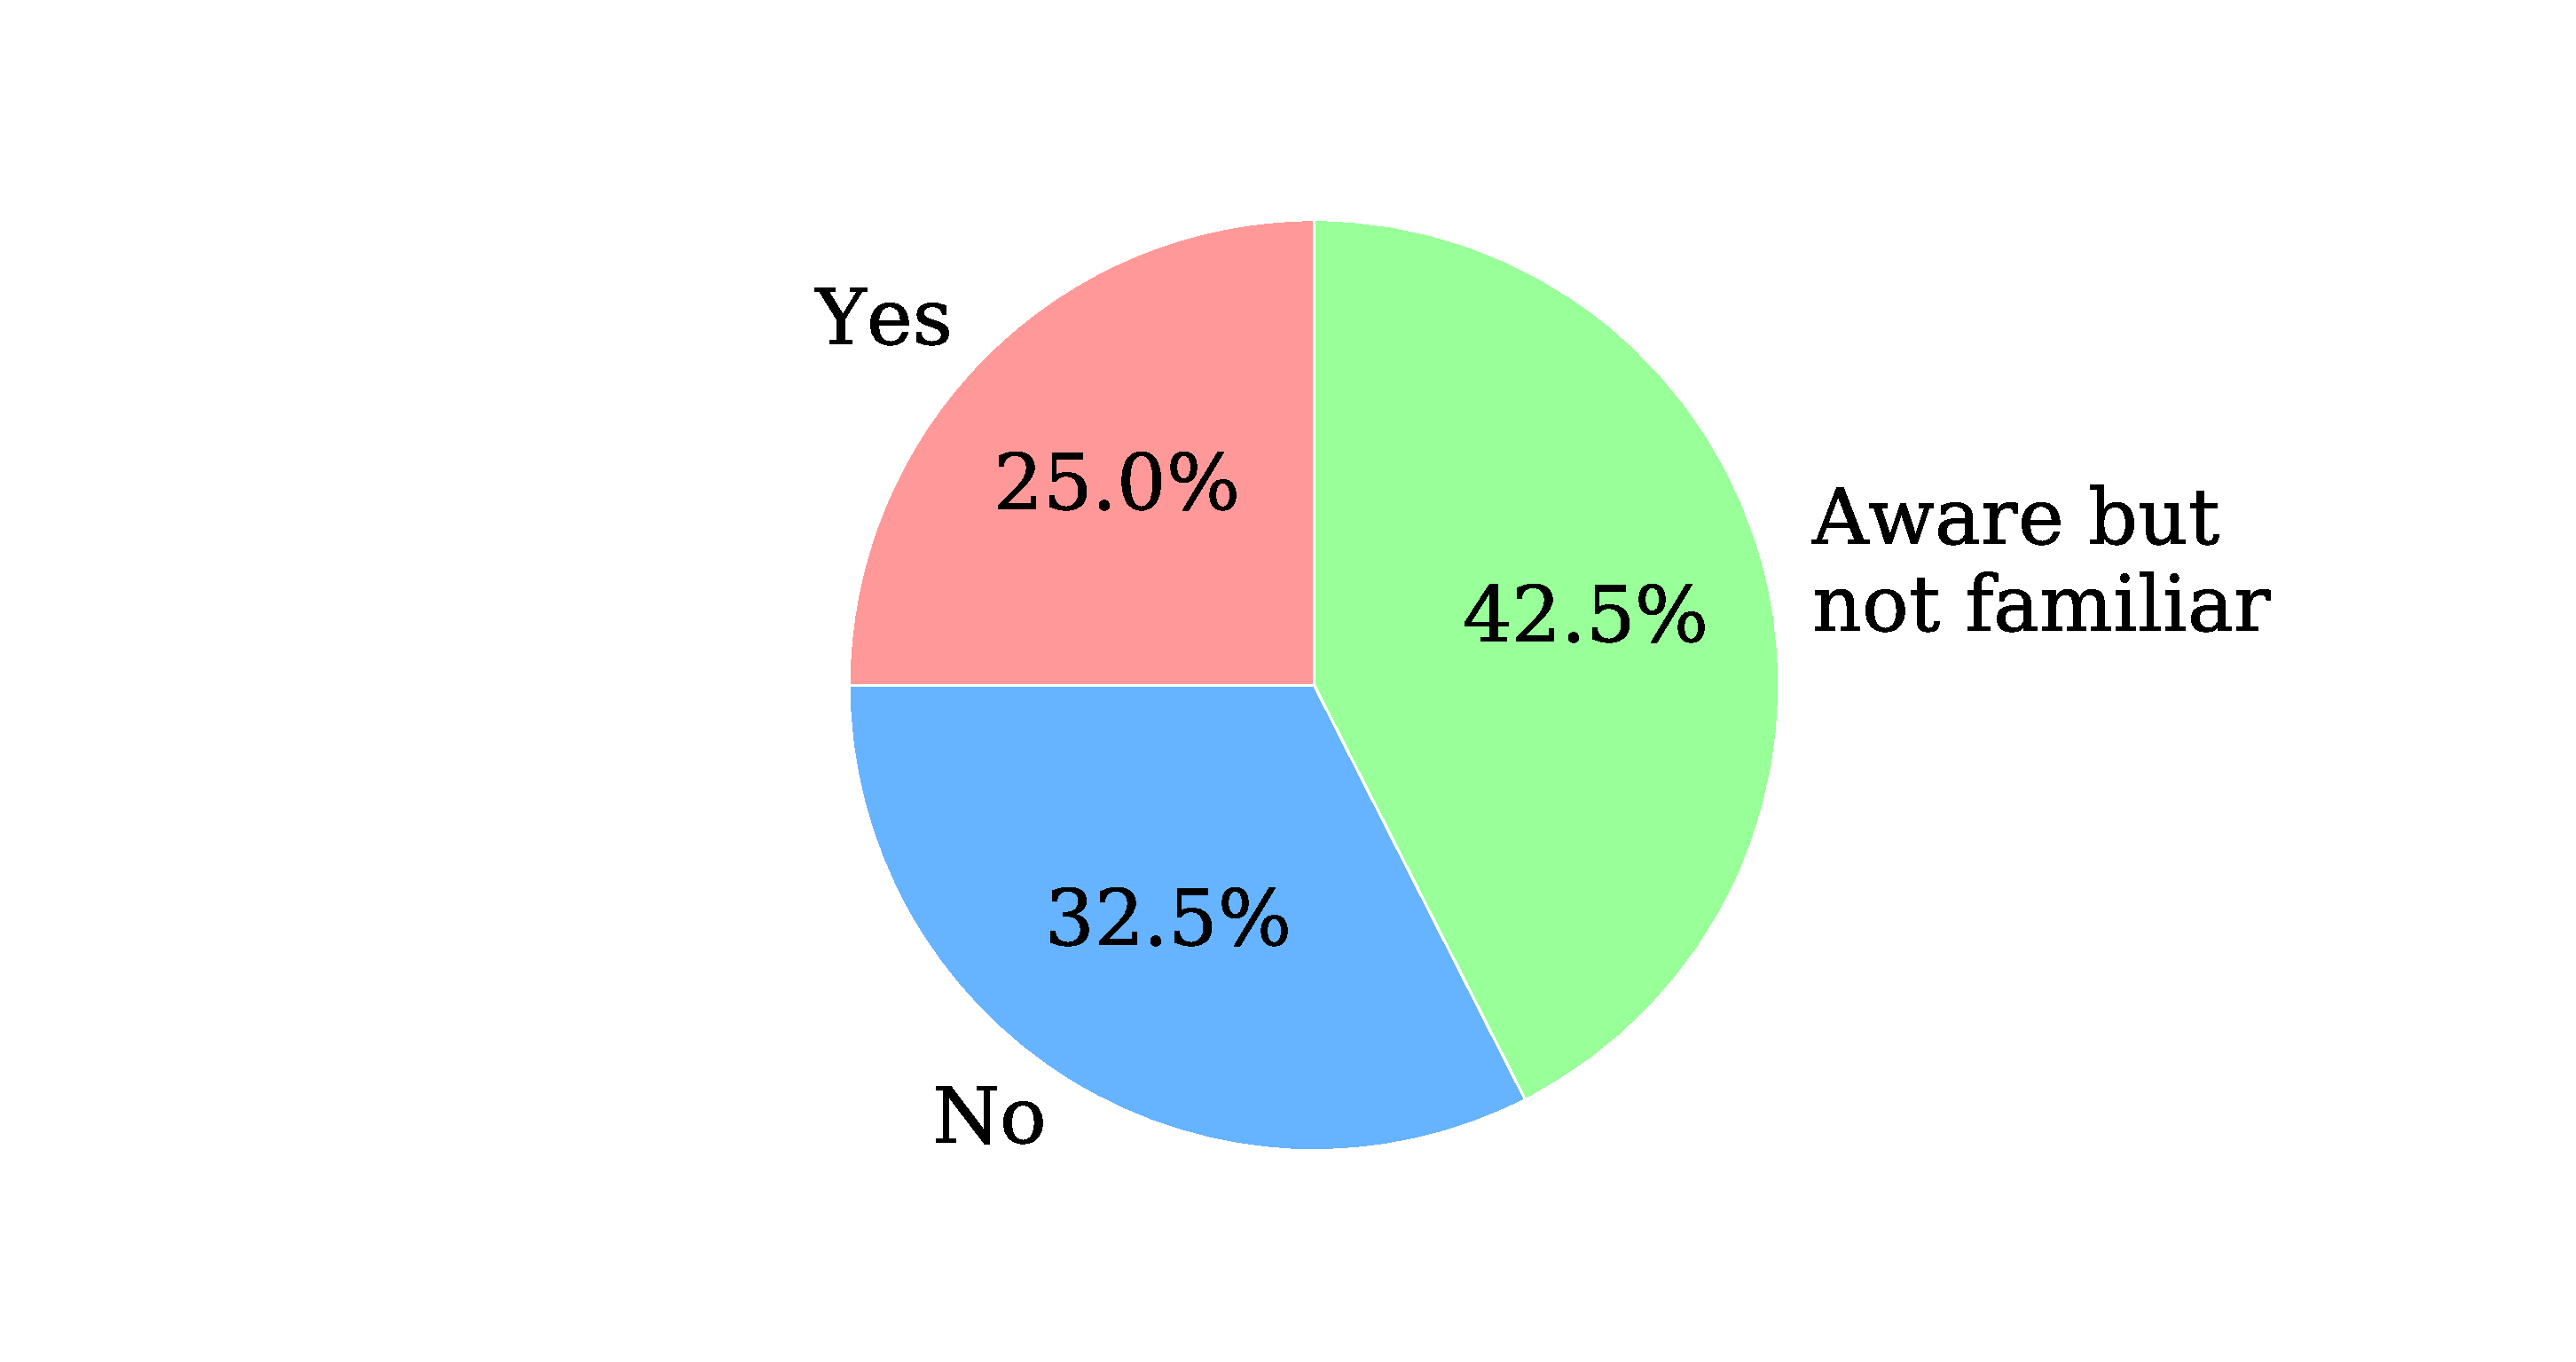
\includegraphics[width=0.6\textwidth]{figures/PAS_1192-2.eps}
	\rule{0.8\textwidth}{0.5pt} % use line???
	\caption{Respondents' familiarity with PAS 1192-2.}
	\label{pas}
\end{figure}


% PIE CHART
\begin{figure}[htbp]
	\centering
	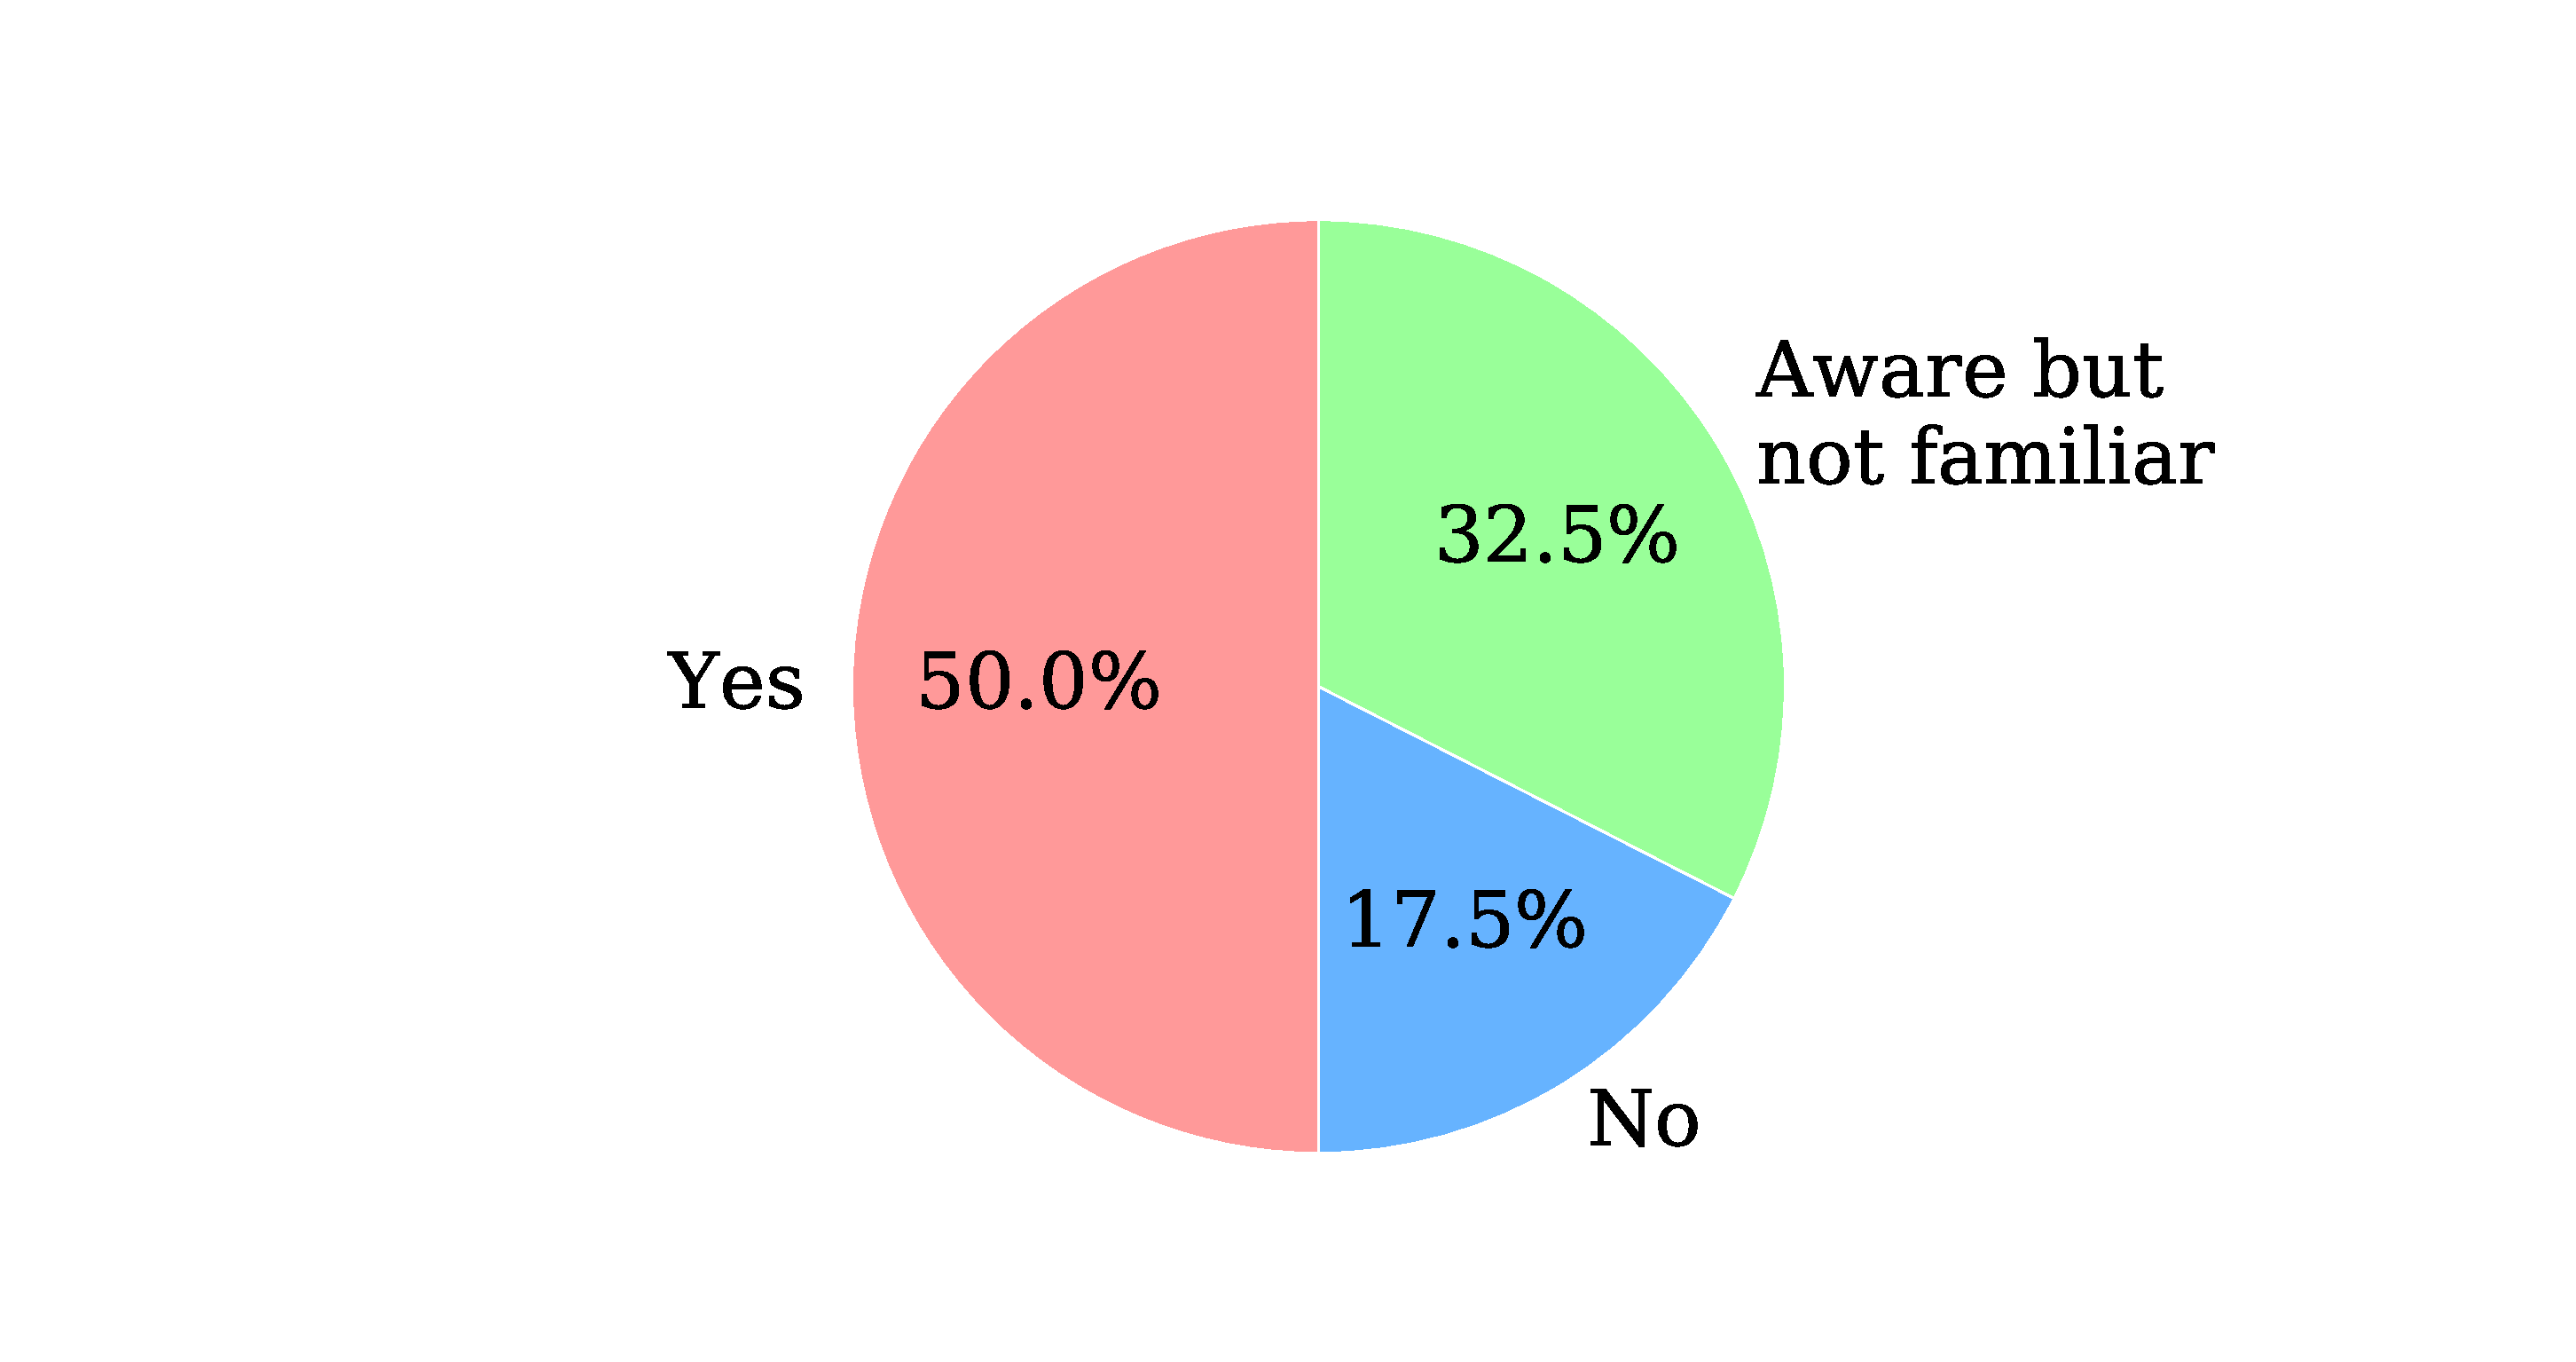
\includegraphics[width=0.6\textwidth]{figures/BG6.eps}
	\rule{0.8\textwidth}{0.5pt} % use line???
	\caption{Respondents' familiarity with BG 6.}
	\label{bg6}
\end{figure}


% PIE CHART
\begin{figure}[htbp]
	\centering
	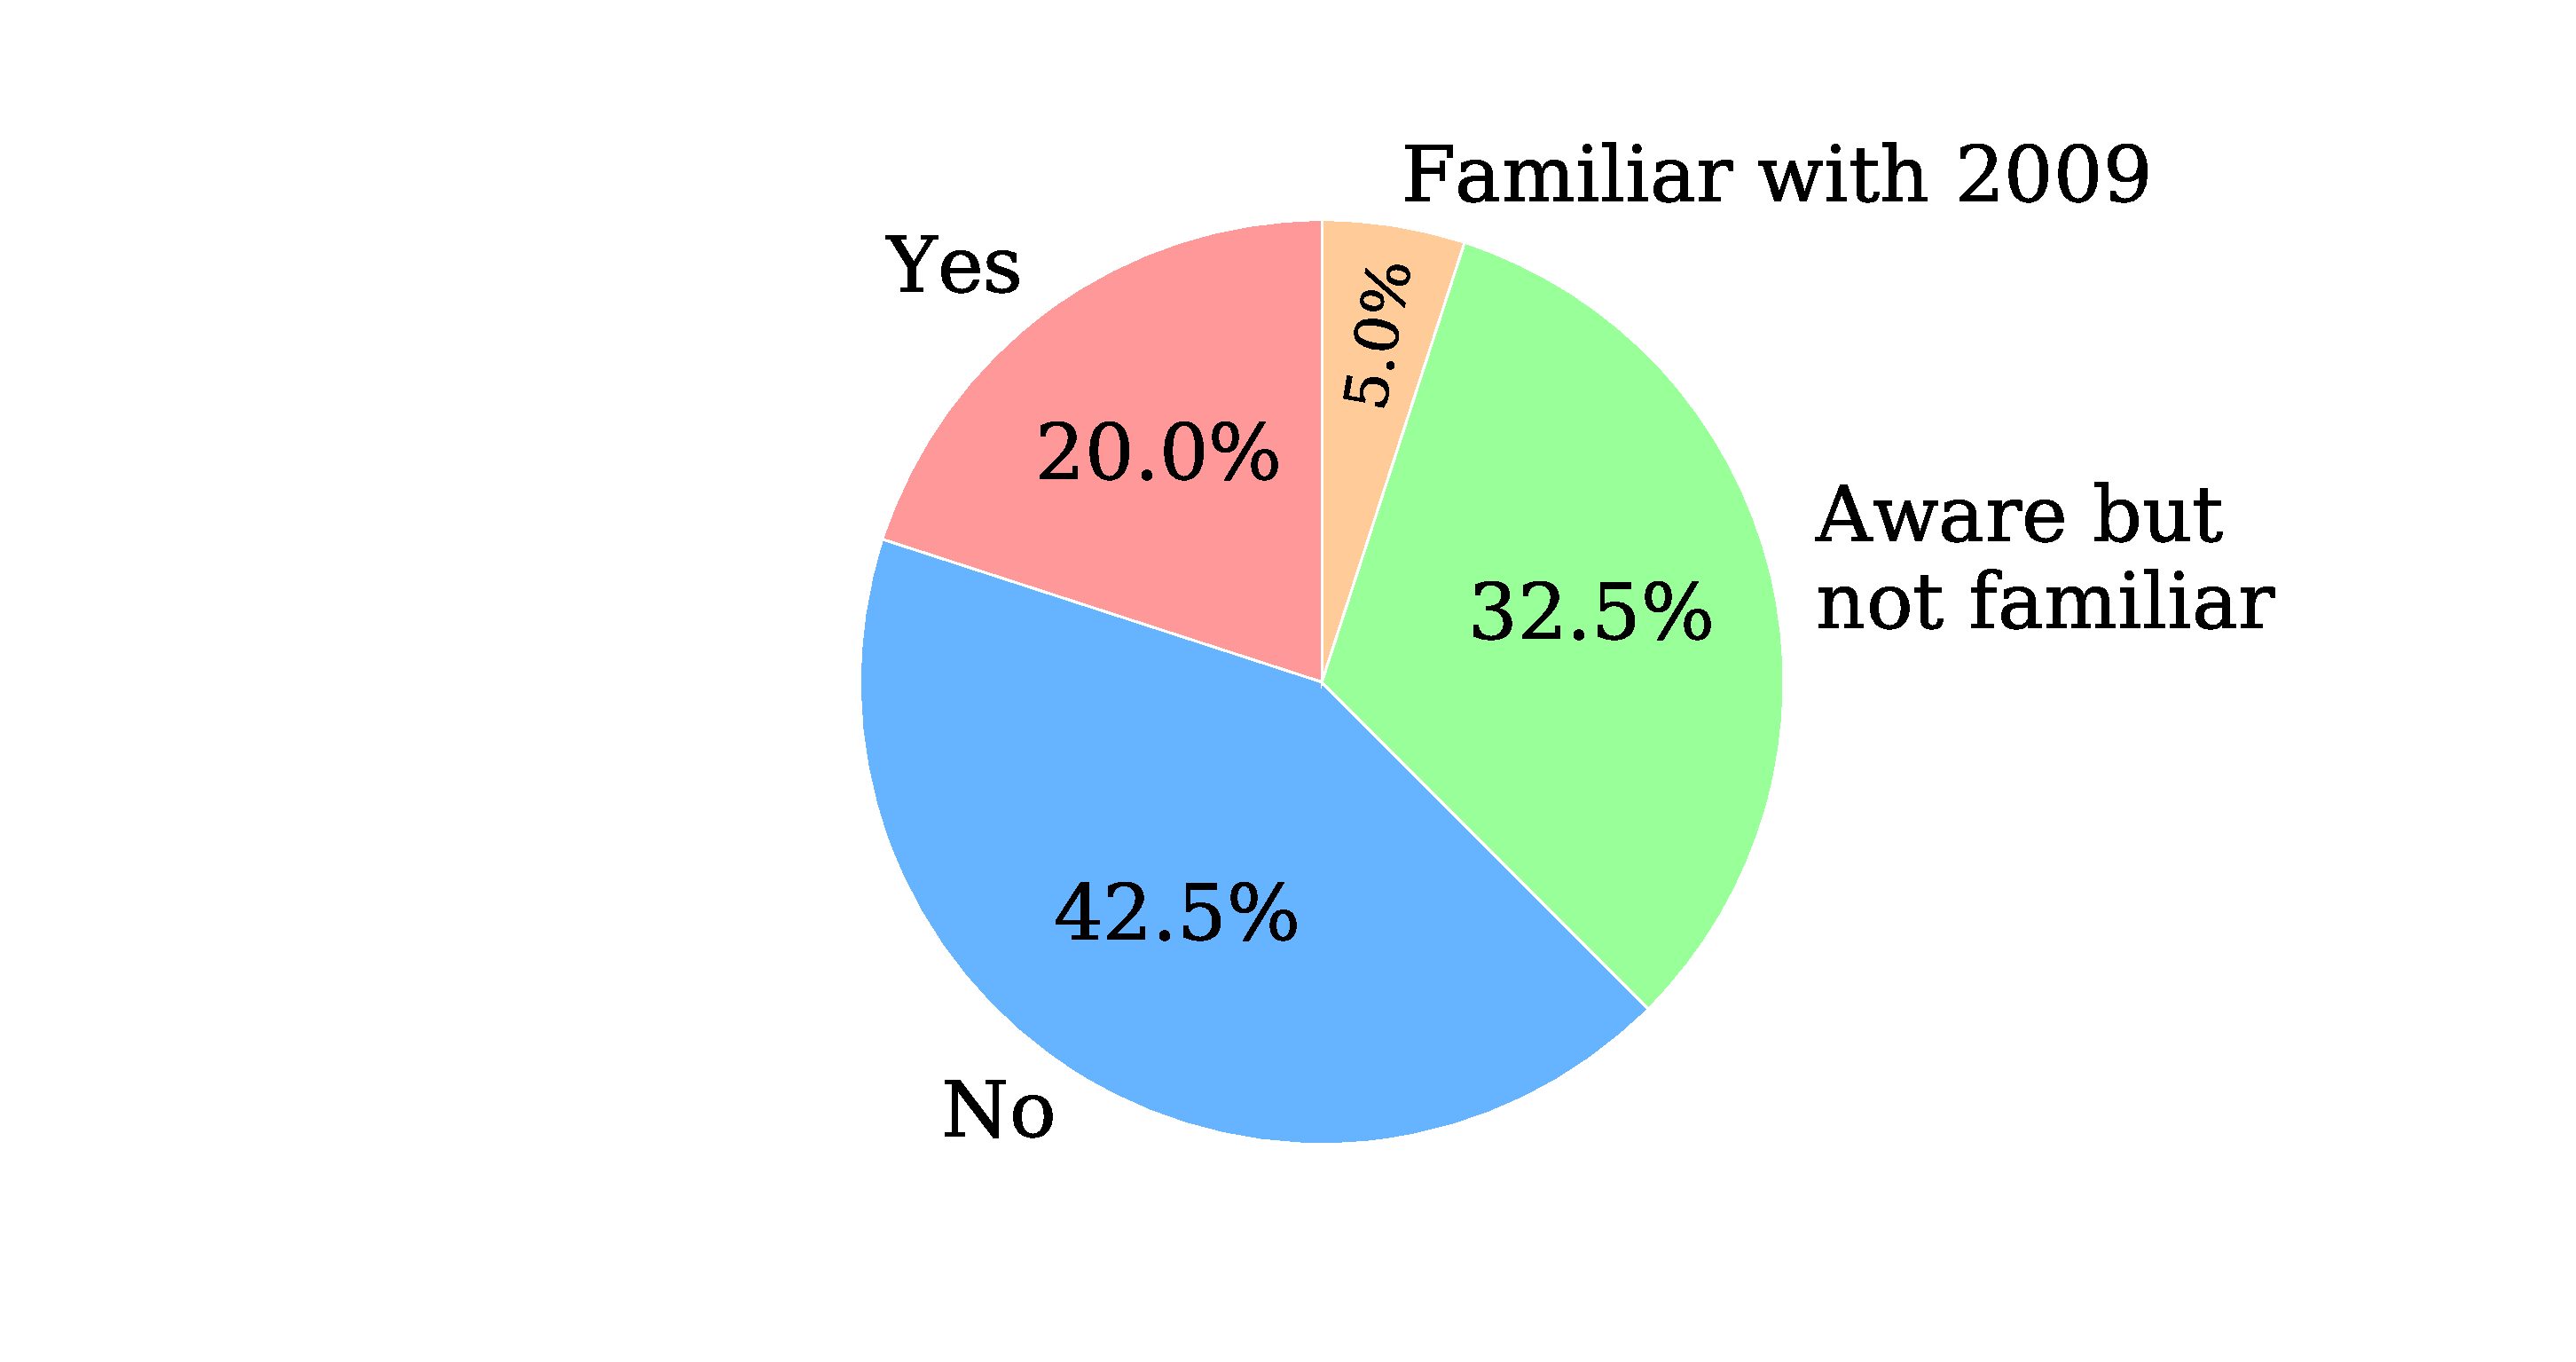
\includegraphics[width=0.6\textwidth]{figures/ACE.eps}
	\rule{0.8\textwidth}{0.5pt} % use line???
	\caption{Respondents' familiarity with ACE Schedule of Services \\ MEP 2017 Edition.}
	\label{ace}
\end{figure}

%% PAS
% 67.5\% of the respondents were aware or familiar with PAS 1192-2.
Figure \ref{BIM_literacy_X_PAS1192} shows the respondents' familiarity with PAS 1192-2 in terms of their BIM literacy.
Since PAS 1192-2 is the industry standard for BIM process during the CAPEX phase of a project, it is interesting to note that 20\% of the respondents agreed to being BIM literate without being familiar with or even aware of the document.
% , yet they have either never heard of or are not familiar with the PAS 1192-2:2013.

% BAR CHART
\begin{figure}[htbp]
	\centering
	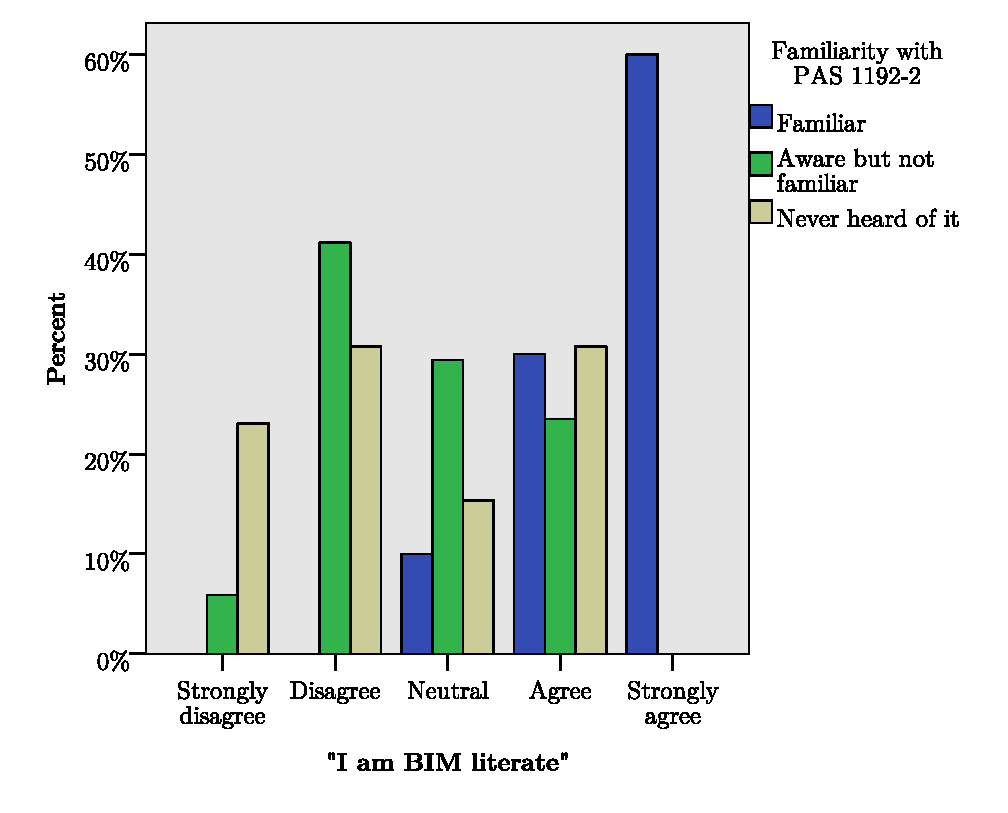
\includegraphics[width=0.9\textwidth]{figures/BimLiteracyXPas1192Percent.eps}
	\rule{0.9\textwidth}{0.5pt} % use line???
	\caption{Respondents' familiarity with PAS 1192-2:2013 in terms of their BIM literacy}
	\label{BIM_literacy_X_PAS1192}
\end{figure}



%% BG6
From Figure \ref{BG6_X_BS_fields} it can be observed that all respondents that have worked in MEP services are aware of or familiar with the BG 6.
% 65.5\% of the MEP respondents are familiar with the document.
Those who have never heard of the BG 6 are composed of specialist building services engineers and people who have not worked in building services.

% BAR CHART
\begin{figure}[htbp]
	\centering
	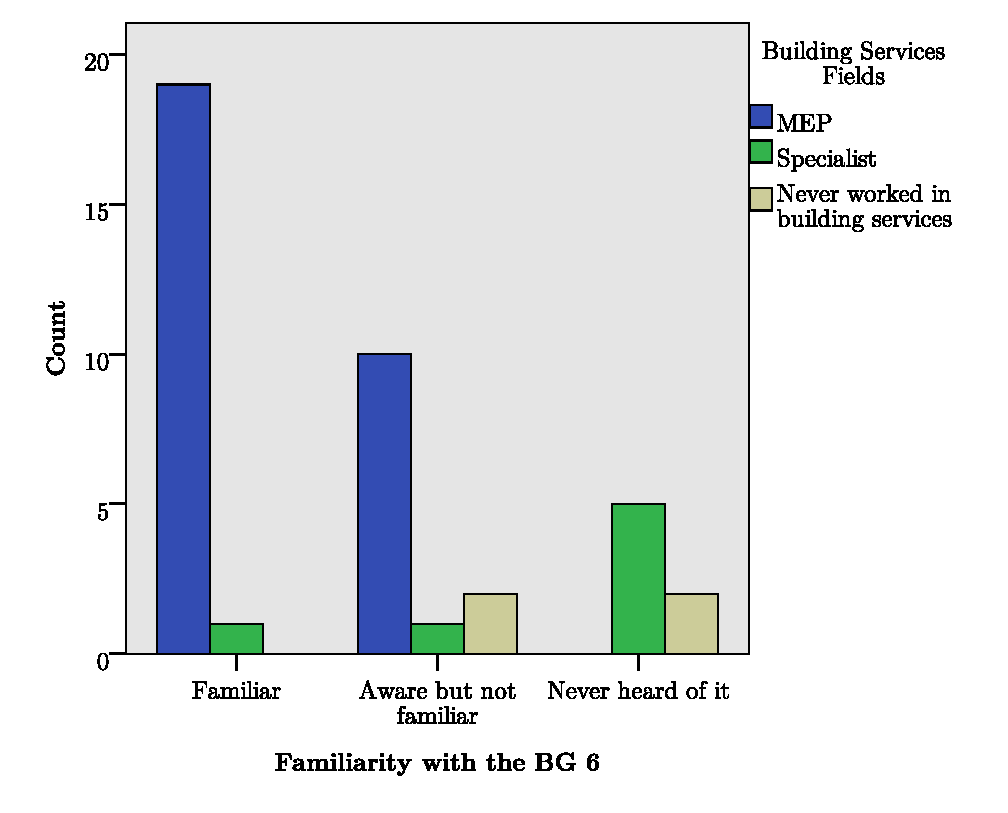
\includegraphics[width=0.9\textwidth]{figures/Bg6XBsFieldsCount.eps}
	\rule{0.9\textwidth}{0.5pt} % use line???
	\caption{Respondents' familiarity with BG6 in terms of building services fields}
	\label{BG6_X_BS_fields}
\end{figure}



%% ACE
Only 25\% of the respondents are familiar with either the 2009 or 2017 (current) edition of the ACE Schedule of Services MEP (see Figure \ref{ace}).
These respondents are either MEP or specialist building services engineers (see Figure \ref{ACE_X_BS_fields}).
As the ACE Schedule of Services MEP is aimed at MEP engineers, it is interesting to note that 72.4\% of the MEP respondents are not familiar with either of the ACE documents.

% BAR CHART
\begin{figure}[htbp]
	\centering
	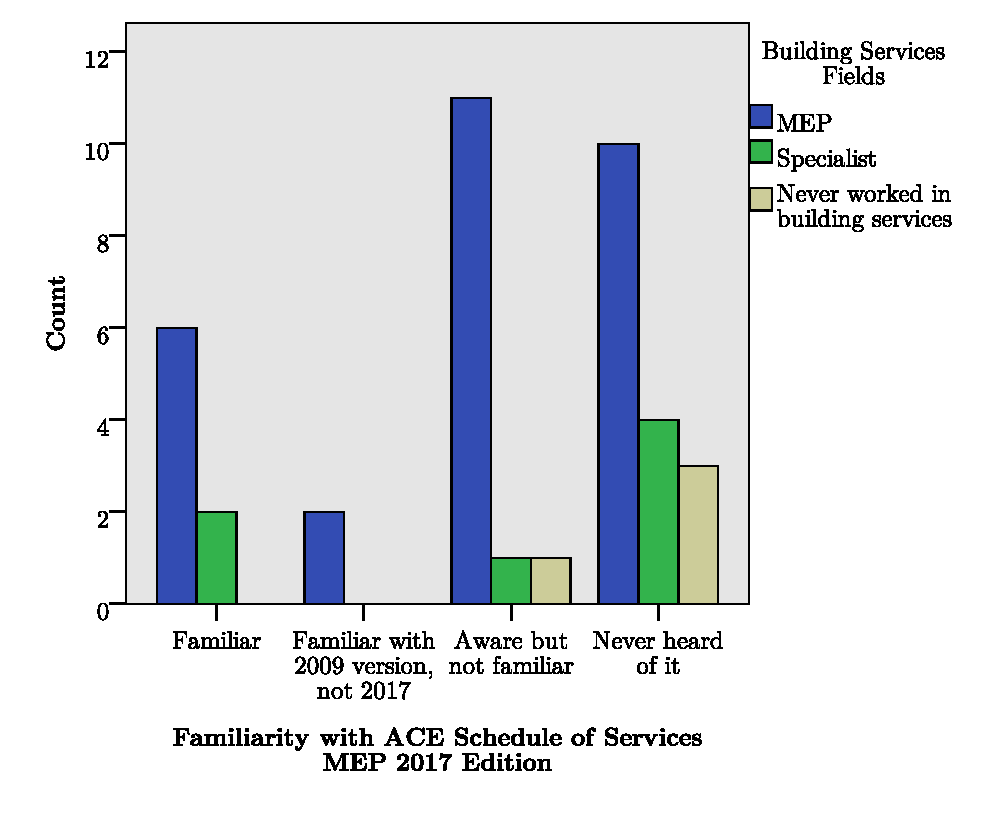
\includegraphics[width=0.9\textwidth]{figures/AceXBsFieldsCount.eps}
	\rule{0.9\textwidth}{0.5pt} % use line???
	\caption{Respondents' familiarity with ACE document in terms of building services fields}
	\label{ACE_X_BS_fields}
\end{figure}








%----------------------------------------------------------------------------------------
%	SECTION 2
%----------------------------------------------------------------------------------------

\section{Follow-Up Interviews}

Four of the survey respondents were approached to participate in follow-up interviews, and two agreed to this.
Both interviewees were experienced MEP contractors: the first worked for a subsidiary of a multinational construction company with over 15,000 employees, and the second worked for a smaller UK construction and engineering company.
The questions used in the interviews can be found in Appendices \ref{AppendixB} and \ref{AppendixC}.

\begin{comment}
\hl{
So far I have identified three people that I would like to have a follow-up interview with: two contractors and one BIM manager/ coordinator.
Should I also speak with a consulting engineer and a policy/ regulation consultant?
If so, perhaps Jon (mechanical engineer, former placement supervisor, plus descriptive in LOD question) and Stefan (consultant)?
(Don't want to have too many interviews to process either...)
}
\end{comment}


%------------------------------
%	SUBSECTION 1
%------------------------------

\subsection{First Interview}

\begin{comment}
\hl{Introduce him...}

MEP contractor.
Work exclusively for LoR.
In other circumstances, would be classed as Tier 2 contractor (sub-contractor to a main contractor).
Primary activity: installation, commissioning and handover of building services on a construction project.
\end{comment}

The first interviewee is the head of information management (a.k.a. BIM management) at their company.
Their team's primary responsibility is the production of information, models and drawings for the installation of MEP services and off-site manufacture.
% Their team produces all the models and drawings for installation and off-site manufacture.
They typically receive information from consultants at Stage 4a (but sometimes also at Stage 3) and develop it to Stage 5.
% at stage 3 or early stage 4, develop it to stage 5.
% More often than not, involved from stage 4a.
However, the interviewee explains that, to make for a practical consultant-to-contractor handover, they would seek to be appointed at Stage 3.
\say{Where we have the opportunity to engage early with our client and the design consultant, for example at Stage 3, then we will be able to influence and guide the development of the model and the design through to Stage 4a. And in those instances we'll get a model that is more useful to us.
Where we enter onto a project where we haven't been engaged early, and we receive a model at Stage 4a, then, more often than not, we need to do a lot of re-work. 
So our strategy is that, where possible, we would like a better quality model that more suits our needs, and if we have the opportunity to engage early, we will try to facilitate that.}

\begin{comment}
Follow BG6 guidance, except they jump from something they receive at 4a straight through to stage 5 (skip 4b and 4c).
They incorporate 4b and 4c in one set of work.
Take 4a model and design, they develop it to have the correct coord for installation adn manufacture. 
They also include all the peculiar (?) equipment and they add all the detail necessary for manufacturing.
They do this all in one process.
\end{comment}

The contractor typically finds that 
the BIM model's intelligence breaks down
when they replace generic objects with specific ones
because it is a \say{replacement rather than an update.}
\say{As soon as you replace an object, it loses the intelligence. That's a fairly major drawback.}
According to them, no one has solved the technical problem yet.
% Would prefer to enhance information rather than replace.
The contractor provides an example of BIM model intelligence breakdown by describing the replacement of an isolating pipe valve in a 4a model.
At this stage, they explain, the consultant does not know who they will procure for the valve.
They will only make that decision once they have been awarded the contract.
However, even if the consultant has not put a generic valve in the model, they will have made an estimate of who the manufacturer would be.
But nine times out of ten, the consultant's chosen manufacturer will be different from what the contractor uses.
At that point, the interviewee needs to take the valve out of the pipe in the model and insert the correct valve; all the intelligence/ information linked to the consultant's valve is lost because the GUID (Globally Unique Identifier)
% (Microsoft's version of UUID)) 
changes.
Every component in the model has a GUID, a hexadecimal number
% / a long string of characters 
that identifies the component.
He says that if you can maintain the GUID, the model will know the information belongs in the same place, but as soon as you replace the object, there is a new GUID. % and \textit{the model cannot remember what it is}.
% GUIDs are generated by the software.
% \hl{Why is there a problem with the GUID changing? If the objects are compatible with each other, and they're all in Revit, and you're inserting an object that you actually need with all of its properties attached to it, what information is being lost?}

% \hl{Perhaps software can be rewritten so that object updates can be done, rather than replacements which require extra work\ldots}

The contractor goes on to explain the ``time-consuming" re-building process of a BIM model.
To re-build a model, they will follow the principles of the design.
So if there are services that are routed above a ceiling down a corridor, then that is the route they will follow.
Thanks to the consultants, the contractor knows where the plant areas are, where the horizontal and vertical distributions are in the building, and they know all the plant sizes from the schematics.
At that point, they will start to re-model using specific equipment and materials, and add in all the details they need for manufacture and installation.
% This is based on the schematic arrangements and the routes given to them in the 4a model.

Regarding BIM software, the contractor said that their team uses
% When asked about the BIM software the contractor's team uses, they said 
Revit MEP and a Revit plug-in called \say{Fabrication Parts} which offers manufacturer-specific objects.

\begin{comment}
One of the government's construction strategies is to enable early contractor involvement \citep{GCS11-15}, which is something contractors themselves seem to prefer according to the follow-up interviewees.
According to \cite{Conaghan2017}, this implies that the government wishes for the MEP consultant to work together with the MEP subcontractor and use the subcontractor's proprietary BIM objects from the outset of a project.
Such a process would streamline the subcontractor's work, who then only has to touch up the model with supports, proprietary information and commissioning data etc.
Another method \hl{John Simpson?} suggests is for the subcontractor to appoint the consultant to work on the BIM model throughout design and construction.

These alternative work processes raise issues about the differences in the knowledge and skill sets of consultants and contractors.
Firstly, consultants do not have the market knowledge \hl{for this} \citep{Conaghan2017}.
Secondly, according to the first follow-up interviewee, the consultant would require the same level of technical knowledge as somebody installing the MEP services on site in order to ``virtually" design and install the services in BIM.
Unfortunately, MEP consultants typically have more of a theoretical knowledge about designing building services, which is inadequate for that technical level of BIM modelling.
Perhaps, as part of implementing the government's construction strategies and improving the productivity of the AEC industry, the line between MEP consultant and contractor needs to blur.
\end{comment}

During the interview, the author brought up the government's wish to enable early contractor involvement.
The author went on to explain that, according to \cite{Conaghan2017}, this implies that the government wishes for the MEP consultant to work together with the MEP subcontractor and use the subcontractor's proprietary BIM objects from the outset of a project.
Upon asking the contractor to comment on this, they indicated that this may not work by raising the problem about 
% Problem about government's wish to use sub-contractors' proprietary objects from project outset is
the differences in skill sets between digital modellers and engineers at a consultancy and at a contractor's.
They said that in order to fulfil the government's wish, there would need to be change or upscaling in personnel to allow the design consultant to model in enough detail for the M\&E contractor.
% Differences in skill sets has to do with having an understanding of installation and manufacture, rather than technical design.
A modeller for an M\&E contractor would require a more practical knowledge (e.g. to understand how services are installed, fitted, built and manufactured).
In other words, a modeller for a contractor would require the same level of knowledge as an on-site engineer installing something, but in a virtual modelling environment.
% In essence, the modeller is engineering and installing virtually rather than out on site.
Unfortunately, MEP consultants typically have more of a theoretical and less of a practical knowledge.

\begin{comment}
Another approach would be for the main contractor to employ a sub-contractor, who themselves would employ the a consultant to carry out the modelling throughout the process.
However, there would be a point where the consultant would hand it over due to differing skill sets.
Or perhaps have a combined resource that sits between the designer and the contractor, to have a broader skill set.
\end{comment}

The contractor finished by describing their process for sending models for automatic fabrication at Stage 5.
They only automate the manufacture of ventilation ductwork.
With this, he explains, ``if you've modelled it very accurately and to certain specifications, then you can export an maj file which can be used by ductwork manufacturing machines that will cut sheet metal and form it into rectangular ductwork."
% .maj is an Autodesk file format (proprietary).
Maj is an Autodesk (thus proprietary) file format which can be exported from the Fabrication Parts plug-in on Revit.
According to the contractor, maj files are typically used in the industry for most ductwork fabrication facilities, and they have not yet encountered any interoperability problems with it.
Once the file is exported as a maj file, there is no manual intervention;
% No manual intervention once exported in .maj format. 
it simply goes into a CNC (Computer Numerical Control) machine and the ductwork is manufactured.


\begin{comment}
The other area of automation is around material take-up: creating schedules of materials and lengths of pipework for cutting.
This isn't automated manufacture, but there is a level of automation that helps the process of manufacture in terms of schedules of materials and procurement.
Nutshell: they can export schedules of materials from the model, and it's imported into a materials procurement system, component by component, then it is … and delivered to the manufacturing facility.
\end{comment}


%------------------------------
%	SUBSECTION 2
%------------------------------

\subsection{Second Interview}

The second interviewee is a senior engineer who currently works as a project manager.
They joined the company as an apprentice and has been worked there for 17 years.
They said that their knowledge in BIM was limited, but that their company was starting to look into delivering a full BIM project.
Despite their limited knowledge in BIM, this contractor has received BIM models from MEP consultants and experienced model intelligence breakdowns.
This, however, was not an issue for the contractor, who did not need to hand it over to the client at the end of the project.
Because the model was only to be used for coordination purposes, the information loss associated with object substitutions was negligible.
% use the model to its full extent or

%------------------------------
%	SUBSECTION 3
%------------------------------

\subsection{Comparison of Interviews}

Despite asking similar questions to both experienced MEP contractors, the author perceived a stark contrast between the two interviews.
There was a noticeable difference in the interviewees' knowledge and awareness of BIM which affected the flow of the conversation.
On the one hand, the first contractor had an advanced knowledge of BIM which allowed the conversation to flow quite well.
On the other hand, the second contractor had a limited knowledge of BIM which caused instances when neither the author nor the contractor could fully understand each other.
This contrast between the interview experiences may reflect the wide range of BIM awareness and knowledge in the industry.


\chapter{Discussion} % Main chapter title

\label{Chapter10} % Change X to a consecutive number; for referencing this chapter elsewhere, use \ref{ChapterX}

\lhead{Chapter 10. \emph{Discussion}} % Change X to a consecutive number; this is for the header on each page - perhaps a shortened title

The collaboration-related guidance offered to the industry has been examined, and the actual communication and collaboration processes of practising building services engineers assessed.
A comparison between industry guidance and practice is conducted and the discrepancies discussed in this chapter.
% The discrepancies that have been identified between industry guidance and practice are discussed in this chapter.


%----------------------------------------------------------------------------------------
%	SECTION 1
%----------------------------------------------------------------------------------------

\section{BIM Awareness and Knowledge}

% Vast variety of BIM awareness and knowledge.
% Cf. questionnaire results + interviews.
% Clients (?) and contractors (e.g. Mark who has never handed over BIM models (as far as he knows/ from what he told me)) not all delivering BIM Level 2 projects that government wants.

The industry's implementation of BIM is the government's solution for the industry to increase its collaboration.
% As of 2016, all public sector projects should be delivered to BIM Level 2 or higher.
However, the ``Industry Practice" assessment in Chapter \ref{Chapter9} revealed a wide range of awareness and knowledge of BIM.
This was evidenced in both the survey and follow-up interviews.
On the one hand, in the survey, 43.6\% of the respondents considered themselves BIM literate, whereas 38.5\% considered themselves BIM illiterate and 18\% neither nor.
Moreover, the survey showed a range of awareness of PAS 1192-2, the industry standard on BIM process during the CAPEX phase of construction projects (see Figure \ref{pas}).
The fact that 20\% of the respondents claimed to be BIM literate without having heard of or being familiar with PAS 1192-2 is a discrepancy itself which suggests a lack of BIM knowledge.
On the other hand, BIM awareness and knowledge was strongly contrasted in the author's interviews with the two experienced contractors.
Whereas the first contractor worked regularly in a BIM environment and was advanced in their BIM knowledge, the second contractor seemed much less aware of both BIM technology and process.

The wide range of BIM awareness and knowledge found in industry practice complies with the literature, in which it was said that BIM adoption was uneven across the industry \citep{DesigningBuildingsLtd2017}.
\cite{Miettinen2014} claimed that it normally takes a company two decades for it to embed a new technology into its work practice from the time the technology is introduced to the company.
The majority of the survey respondents started working with BIM sometime since 2011 (i.e. seven years ago), the year the \citeauthor{GCS11-15} mandated BIM Level 2 (see Figure \ref{bim_yrs}).
Therefore, it might not be until the 2030s (i.e. two decades later) that BIM technology and process are fully embedded into the work practices of UK AEC companies.


%----------------------------------------------------------------------------------------
%	SECTION 2
%----------------------------------------------------------------------------------------

\section{Consultant-to-Contractor Handovers}


%----------------------------
%	SUBSECTION 1
%----------------------------

\subsection{Prevention of Smooth Handovers Due to a Lack of Interoperability}

At Stage 4a, the BG 6 recommends the following to building services engineers:
``Where there is no MEP contractor selected, the design will use generic or typical components, that may be substituted during equipment procurement" \citep[p.~54]{BG62014}.
However, in reality, these substitutions can be more complicated and time-consuming than the BG 6 makes it sound.
According to the first follow-up interviewee, current BIM technology does not support intelligent substitutions of objects.
Therefore, in order to maintain the integrity and intelligence of a BIM model, it seems that most contractors are forced to re-build the entire model from scratch.

The value of contractors re-building BIM models is debatable.
On the one hand, the re-building process is inefficient because it requires extra time and effort to design the same thing over again.
The re-work thus goes against one of the purposes of BIM, which is to streamline the design process.
For this reason, clients could argue that contractors should not get paid to essentially \emph{re-do} the consultants' work.
% Contractors doing work over again because of not being able to do intelligent substitutions in BIM model.
% One can speculate that they're not paid to do this re-work either…
% There is an element of re-work/ inefficiency here which the concept of BIM is supposedly supposed to eliminate.
On the other hand, re-building the BIM model could be regarded as a valuable exercise for contractors, especially when the MEP design is complicated.
The act of re-building forces contractors to go over every detail of the design, thus allowing them to validate and intimately familiarise themselves with the design.
This could make for a smoother transition to construction and installation by avoiding unexpected mistakes and costs.
Therefore, the re-building activity may also be financially beneficial for clients.

In contrast, the lack of interoperability may not be a problem in cases where clients do not require intact BIM models.
Instead, BIM models might simply be used for coordination purposes, whereby breakdowns of model intelligence are negligible.
However, the absences of BIM model integrity and handover to the client do not comply with BIM Level 2 project delivery.

BuildingSMART has adopted a standard that allows the sharing of incremental changes in BIM models, as opposed to sharing entire models which might easily be several megabytes (MB) large.
This standard is called the Open BIM Collaboration Format (BCF) \citep{Bosche, buildingsmart}.
According to \cite{Bosche}, the use of BCF is not yet widespread, but it is anticipated that it will soon be prevalent in the industry as part of BIM Level 3.
Perhaps a version of BCF or a similar technology exists or should be developed to allow for the updating of BIM objects from generic to specific.

% Technologies seem to have linear thinking, i.e. not designed for feedback loops, changes or re-work.
% This goes against the concept of iterations in design.
% There is a similar technology that exists already as part of IFC by buildingSMART: BCF.
% Incremental changes…



%----------------------------
%	SUBSECTION 2
%----------------------------

\subsection{Consultant Vs. Contractor Knowledge and Skill Sets}

One of the government's construction strategies is to enable early contractor involvement \citep{GCS11-15}, which is something contractors themselves seem to prefer according to the follow-up interviewees.
According to \cite{Conaghan2017}, this implies that the government wishes for the MEP consultant to work together with the MEP subcontractor and use the subcontractor's proprietary BIM objects from the outset of a project.
Such a process would streamline the subcontractor's work, who then only has to touch up the model with supports, proprietary information and commissioning data etc.
Another method that was suggested to the author is for the subcontractor to appoint the consultant to work on the BIM model throughout design and construction.

These alternative work processes raise issues about the differences in the knowledge and skill sets of consultants and contractors.
Firstly, consultants do not have the market knowledge for this \citep{Conaghan2017}.
Secondly, according to the first follow-up interviewee, the consultant would require the same level of technical knowledge as somebody installing the MEP services on site in order to virtually design and install the services in BIM.
Unfortunately, MEP consultants typically have more of a theoretical knowledge about designing building services, which is inadequate for that technical level of BIM modelling.
Perhaps, as part of implementing the government's construction strategies and improving the productivity of the AEC industry, the line between MEP consultant and contractor needs to blur.

The blurring of the line between MEP consultants and contractors could potentially have social ramifications within the industry.
The traditional procurement route can be seen as being predicated on RIBA's $ 19^{th} $ century hierarchical notions, whereby the architect assembles a team to produce the drawings, which are passed on to the contractor who gets the builders to construct the facility accordingly.
Meanwhile, the client sits back and does not get very involved.
However, it looks like some of the assumptions made in the industry about those roles may be outdated today.
Now, there is a movement in the industry, initiated by the likes of \citeauthor{Latham1994} and \citeauthor{Egan1998}, to improve communication and collaboration, put the client in the centre, and involve the contractor earlier etc.
This movement is arguably flattening the hierarchy around which the RIBA PoW stages were established.
It is possible that some MEP consultants may interpret this as them losing stature, which they may find incommodious, unfair, and/ or offensive.

% Possible ramifications on regard/ pride of graduate engineers/ CIBSE members. 
% (prejudice?)
% One could argue that the current communication/ collaboration processes we are working in are predicated/ based on a 19th century (when RIBA was founded) set of values where architect assembles the team who produces the drawings which are passed on to the contractor who get the little people to build them.
% Meanwhile, the client is not very involved.
% Government wants to implement early contractor involvement.
% According to Paddy, it is implied that sub-contractors' proprietary BIM objects are used from start.
% \hl{John Simpson?} says this could possibly work if SC appoints consultant who carries out modelling throughout design and construction.
% Martin raises problem of difference in skill set between consultants and contractors.
% Install virtually…
% Line between consultant and contractor needs to blur.



% But involve the contractor too early, he may have a lazy attitude and will not push the envelope...


%----------------------------------------------------------------------------------------
%	SECTION 3
%----------------------------------------------------------------------------------------

\section{Data Exchange Through Proprietary File Formats}

\cite{NBS2014} defines BIM Level 2 as distinguished by collaborative working by which design information is shared through common file formats such as IFC.
However, according to \cite{Laakso2012} and the first follow-up interviewee, proprietary file formats are still in use.
The interviewee reported that the maj file format by Autodesk is typically used in the industry for most ductwork fabrication facilities.
The persistent use of proprietary file formats does not fully comply with BIM Level 2.
Although the interviewee had never encountered interoperability problems when using the maj file format, such issues might arise when using different BIM software programmes or CNC machines for automatic fabrication purposes.
% However, it is possible that common file formats are not needed for certain operations, such as automatic fabrication, if proprietary formats like maj are standardised in the industry.
% and they have not yet encountered any interoperability problems with it.

\begin{comment}
The contractor finished by describing their process for sending models for automatic fabrication at Stage 5.
They only automate the manufacture of ventilation ductwork.
With this, he explains, ``if you've modelled it very accurately and to certain specifications, then you can export an maj file which can be used by ductwork manufacturing machines that will cut sheet metal and form it into rectangular ductwork."
% .maj is an Autodesk file format (proprietary).
Maj is an Autodesk (thus proprietary) file format which can be exported from the Fabrication Parts plug-in on Revit.
According to the contractor, maj files are typically used in the industry for most ductwork fabrication facilities, and they have not yet encountered any interoperability problems with it.
Once the file is exported as a maj file, there is no manual intervention;
% No manual intervention once exported in .maj format. 
it simply goes into a CNC (Computer Numerical Control) machine and the ductwork is manufactured.
\end{comment}

%----------------------------------------------------------------------------------------
%	SECTION 4
%----------------------------------------------------------------------------------------

\section{Confusion with LODs}

LODs were introduced as a tool to improve the quality of communication among BIM users about the characteristics of the graphical and non-graphical content in BIM models.
However, the LOD terms seem to have created even more confusion.
LODs get mistaken for meaning coordination, the terms themselves can be ambiguous (e.g. does level of detail mean LoD or extent of information?), and they can erroneously get associated with work stages.
\begin{comment}
\begin{itemize}
	\item People mistaking LODs for coordination
	\item Association with work stages
		\begin{itemize}
			\item No clear coherence in various industry guidance documents
			\item Same numbers in UK and similar in USA (2, 3, 4 etc.)
			\item Blanket value issue
			\item Employers' misunderstanding/ confusion
		\end{itemize}
	\item Terms themselves are ambiguous (level of detail - LoD or extent of info?)
\end{itemize}

Don't actually know whether clients typically comply with industry guidance regarding setting LODs at start of projects.
However, I've been told on more than one occasion (\cite{Quigley2017} and Jon) that there is a range in clients' and/ or contractors' understanding of LODs, and thus a large range in the quality of EIRs.

PAS 1192-2, BG 6 and the NBS article were respectively published in 2013, 2014 and 2015, whereas CIBSE DE2 and the ACE Schedule of Services MEP were respectively published in 2016 and 2017.
There appears to be a correlation between the publication dates of these documents and their guidance on whether LODs are work stage related.
This may suggest that the industry realised in 2016 that LODs should not be work stage related.
%However, this is purely speculation made without any firm evidence.
More recent publications by BSI, BSRIA and NBS might confirm this speculation.
\end{comment}


%----------------------------
%	SUBSECTION 1
%----------------------------

\subsection{Poor or Pertinent Names?}

At least 90\% of the survey respondents correctly matched the terms LoD and LoI to graphical and non-graphical content, respectively, despite the fact that only 60\% of the respondents were familiar with the terms.
These results indicate that the terms may be aptly suited to their definitions.
However, the terms LoD and LoI are ambiguous because they can be used interchangeably with the common phrases ``level of detail" and ``level of information" which may not strictly refer to either the graphical or non-graphical content of BIM models.
This is unfortunately what is done in the industry guidance documents.
Therefore, to increase clarity, perhaps more pertinent and unique names should be given to describe the amount of graphical and non-graphical content in BIM models.
% Most of survey respondents associated LoD and LoI correctly with graphical and non-graphical information, respectively.
% However, author's confusion of use of phrase ``level of detail" in reading guidance documents.
% Also, association with work stages.



%----------------------------
%	SUBSECTION 2
%----------------------------

\subsection{Project- or Stage-Related?}


There appears to be a disagreement within the industry guidance documents on whether LODs are project- or stage-related.
The work stage association is due to organisations such as the BSI, BSRIA and NBS associating LODs with work stages in PAS 1192-2, BG 6 and NBS BIM Toolkit, respectively.
The work stage association is also due to the resemblance of the LOD numbers to the numbers of the RIBA PoW and CIC Scope of Services stages.
It is therefore not surprising that clients may misunderstand the meaning of LODs and that they should define LODs as blanket values for the whole project, changing at each stage.
Moreover, the `Match the Image with the Work Stage' activity in the questionnaire showed that there was a general agreement among the respondents about the amount of graphical content that the NBS and BSRIA expect at various work stages.
% It is likely that these respondents work regularly with BIM production or designing to meet LODs. 
Despite all this, the ACE Schedule of Services MEP, CIBSE DE2 and the majority of the respondents to the open-ended question “Have you noticed a difference in levels of definition from one project to the next?” agree that LODs are project-related, not stage-related.
This dissonance resonates with something a policy and regulation consultant said in the survey: ``there is no actual definition of what the various LoDs mean, the interpretation always varies, though there are similar themes".

% There is no actual definition for LODs...
Perhaps 
% author (and clients) initially misinterpreted LODs as defined in industry guidance to be stage-related.
LODs should be interpreted as follows:
LODs are simply a set of categories of various progressions of BIM model content that one can choose from and apply to different aspects of design work.
They would be typically used to communicate how much content the model should have by the end of a work stage.
This wouldn't mean that NBS LoI 4 should apply to Stage 4 for all design aspects across all construction projects.

LODs need to be more clearly defined in the guidance documents.
Otherwise, perhaps the whole concept of LODs should be replaced by a more effective communication system for BIM.
% is confusing and should be scratched (refer to BIM manager that has alternative approach to LODs).

\chapter{Conclusion} % Main chapter title

\label{Chapter11} % Change X to a consecutive number; for referencing this chapter elsewhere, use \ref{ChapterX}

\lhead{Chapter 11. \emph{Conclusion}} % Change X to a consecutive number; this is for the header on each page - perhaps a shortened title

% The aim of this research study is to investigate the discrepancies between industry guidance and practice in building services engineers' processes for collaboration in the UK.
% To provide context before the discrepancies are sought, the concept of collaboration will be explored, along with the collaboration-enabling tools on the market for building services engineers.

This study revealed five discrepancies between industry guidance and practice in building services engineers' processes for collaboration in the UK.
The first is the government's request for the widespread adoption of BIM since 2016, yet there is still a wide range of BIM awareness and knowledge in the industry.
The second is the BG 6's recommendation of substituting generic BIM objects with specific BIM objects during equipment procurement, but this is technically not possible at the moment.
Instead, the lack of BIM interoperability is engendering a time-consuming process of re-work. %, the value of which is arguably wasteful or beneficial in the long-term.
The third is the government's request for early contractor involvement and the use of proprietary BIM objects from the outset of a project, which requires a practical knowledge and skill set.
This conflicts with the purely theoretical knowledge and skill set of most consultants, if the consultants are the ones to be designing the building services at the start of a project.
The fourth is the industry's continued use of proprietary file formats (e.g. maj) in spite of the government's request to deliver projects to BIM Level 2, which is distinguished by data exchange through common file formats (e.g. IFC).
The fifth (and last) is the industry's introduction of LODs to facilitate communication among BIM users, yet in reality, the LOD terms seem to have caused more confusion.

The implications of these discrepancies are varied.
The contractor's re-work engendered from BIM interoperability is arguably inefficient or valuable for making a smoother transition to construction and installation.
The government's construction strategies suggest an imminent social reformation of the UK's AEC industry, which may disgruntle certain professionals who consider themselves high up in the current hierarchy.
% request for early contractor involvement among other things is a signs of a potential upcoming reformation of the UK AEC industry
The abortive introduction of the LOD terms might instigate the creation of a more effective communication system for BIM.
With BIM being a recent innovation in both technology and process, its implementation in the industry is itself a sort of design exercise.
It will require iterations of trial and error before (a) the industry gets accustomed to BIM process and technology and (b) the industry is able to adapt BIM technology and process to suit its needs.
% The implementation of the BIM process is a design exercise in itself, with iterations to see which processes work and which do not…
As \cite{Miettinen2014} suggest, this `design exercise' may take up to two decades.
% Practice makes perfect?

%----------------------------------------------------------------------------------------
%	SECTION 1
%----------------------------------------------------------------------------------------

\section{Limitations of Current Research}

Limitations in this study included time and resources.
These could have contributed to getting a larger sample size for the survey.
If a greater sample size that is less skewed and more representative of the UK population of building services engineers could have been acquired, more advanced and accurate statistical analysis could have been conducted.
% Such statistical analysis include 
% If the author and the supervisor could have reached out to a greater number of practising AEC professionals, perhaps 
Also, with more time, it would have been interesting to follow-up more responses from the survey, for example to acquire more examples on how LODs are project-related and not stage-related.

% Although many in industry claimed/ expressed that LODs are project related, not work stage related, I have limited examples to demonstrate this.

% Somehow include flow charts drawn in pencil of stage to stage interactions within various disciplines which confirms info exchanges…

%----------------------------------------------------------------------------------------
%	SECTION 2
%----------------------------------------------------------------------------------------

\section{Suggestions for Further Research}

It might be interesting to investigate the information flow patterns between MEP consultants and contractors in order to identify characteristics that would facilitate the development of more effective CSCW tools.
A variant of this suggestion would be to examine the implications of the technology that enables intelligent object substitutions in BIM models, if or when this technology emerges.
It would be interesting to compare the consultant-to-contractor handover process with and without that technology (e.g. the extent of re-work on the BIM model, the number of hours worked by the contractors, and the smoothness of the transition to construction and installation on site).
Such a study would contribute to streamlining the handover process. % smoother and more efficient.

Other suggestions for further research that have resulted from the discoveries and limitations of this study are:
\begin{itemize}
	\item Further research into the development, evolution and effectiveness of LODs in the UK's AEC industry.
	This could involve investigating the sources of confusion with LODs, whether their meaning has evolved from being stage- to project-related, and exploring other means of communicating the amounts of graphical and non-graphical content in BIM models.
	The latter could include identifying alternative approaches that are currently being employed in the industry and assessing their efficiency compared to LODs.
	% Explore other means of communicating amount of model detail and information, e.g. by seeing alternative approaches currently being employed in industry (are these more efficient?).
	% More recent publications by BSI, BSRIA and NBS might confirm this speculation (This may suggest that the industry realised in 2016 that LODs should not be work stage related.)
	% LODs mistaken for coordination - how exactly?
	% Investigate sources of confusion of or problems with LODs.
	
	\item ``Does the line between building services consultants and contractors need to blur for improved productivity?" The `blurring line' could manifest itself through MEP consultants gaining more practical knowledge and/ or an increased collaboration between consultants and contractors.
	Such a study could explore the implications related to productivity, social hierarchy, technology and education.
	
	\item ``To what extent have building services engineers achieved BIM Level 2 in the UK?" As BIM Level 2 is distinguished by data exchange through common file formats, this study would involve examining how practising building services engineers are exchanging design information.
\end{itemize}

% Big range of BIM awareness discovered - further study extent of BIM technology and BIM process knowledge in industry?


% stakeholders on a construction project.

\begin{comment}
TEST: if/ when the technology emerges to make intelligent object substitutions in BIM models, compare the
(1) productivity of construction projects/ 
(2) efficiency of handover (e.g. compare number of hours worked)/ 
(3) how well the contractor works on site in the following scenarios:
\begin{itemize}
	\item The contractor simply substitutes the generic BIM objects with specific ones without doing any form of re-work
	\item The contractor re-builds the model (like they do today), learning the design intimately
\end{itemize}
\end{comment}

% How information is lost during handovers?


%----------------------------------------------------------------------------------------
%	THESIS CONTENT - APPENDICES
%----------------------------------------------------------------------------------------

\addtocontents{toc}{\vspace{2em}} % Add a gap in the Contents, for aesthetics

\appendix % Cue to tell LaTeX that the following 'chapters' are Appendices

% Include the appendices of the thesis as separate files from the Appendices folder
% Uncomment the lines as you write the Appendices

% Appendix A

\chapter{Questionnaire} % Main appendix title

\label{Questionnaire} % For referencing this appendix elsewhere, use \ref{AppendixA}

\lhead{Appendix A. \emph{Questionnaire}} % This is for the header on each page - perhaps a shortened title

This appendix contains the questionnaire that was used in the survey (starts on following page).
The questionnaire is described in detail in Section \ref{sec_survey}.
The digital version of the questionnaire that was shared with all survey invitees can be found at: \url{https://docs.google.com/forms/d/e/1FAIpQLSe53m6rMGQV0iB8JNoVvbeoGAov7DAYEvlJnyowNDuRzuPoqg/viewform?c=0&w=1}.

\includepdf[pages=-]{Appendices/Questionnaire_margins_adapted.pdf}
% Appendix B

\chapter{Interview 1 Questions} % Main appendix title

\label{AppendixB} % For referencing this appendix elsewhere, use \ref{AppendixA}

\lhead{Appendix B. \emph{Interview 1 Questions}} % This is for the header on each page - perhaps a shortened title

This appendix contains the questions that were used in the first follow-up interview.

\includepdf[pages=-]{Appendices/Interview1.pdf}
% Appendix C

\chapter{Interview 2 Questions} % Main appendix title

\label{AppendixC} % For referencing this appendix elsewhere, use \ref{AppendixA}

\lhead{Appendix C. \emph{Interview 2 Questions}} % This is for the header on each page - perhaps a shortened title

This appendix contains the questions that were used in the second follow-up interview.

\includepdf[pages=-]{Appendices/Interview2.pdf}

\addtocontents{toc}{\vspace{2em}} % Add a gap in the Contents, for aesthetics

\backmatter

%----------------------------------------------------------------------------------------
%	BIBLIOGRAPHY
%----------------------------------------------------------------------------------------

\label{Bibliography}

\lhead{\emph{References}} % Change the page header to say "Bibliography"

\bibliographystyle{apalike} % Use the "apalike" BibTeX style for formatting the Bibliography

\bibliography{Bibliography} % The references (bibliography) information are stored in the file named "Bibliography.bib"

\end{document}